\documentclass[british,titlepage]{ntnuthesis}

\begin{figure}
\hspace{-2cm}
    
\includegraphics[scale=.6]{figures/logo_ntnu_eng.png}
\end{figure}


\title{\LARGE \textbf{Investigating potential immunotoxic and genotoxic effects of chronic exposure to wastewater-aged engineered nanoparticles in \emph{M. edulis} haemocytes}}
\shorttitle{ENVITOX Master Thesis}
\author{Tørris Sandsæter}
\shortauthor{T. Sandsæter}
\date{\today}

\addbibresource{nonauto.bib}



% From https://www.overleaf.com/learn/latex/Glossaries

\makeglossaries % Prepare for adding glossary entries


\newglossaryentry{latex}
{
        name=latex,
        description={Is a mark up language specially suited for
scientific documents}
}

\newglossaryentry{bibliography}
{
        name=bibliography,
        plural=bibliographies,
        description={A list of the books referred to in a scholarly work,
typically printed as an appendix}
}

\newglossaryentry{maths}
{
    name=mathematics,
    description={Mathematics is what mathematicians do}
}


% --------------------
% ----- Acronyms -----
% --------------------

\newacronym{phd}{PhD}{philosophiae doctor}
\newacronym{CoPCSE}{CoPCSE@NTNU}{Community of Practice in Computer ScienceEducation at NTNU}
\newacronym{gcd}{GCD}{Greatest Common Divisor}
\newacronym{ethd-1}{EthD-1}{Ethidium Homodimer-1}
\newacronym{FCM}{}{Flow cytmeter}
%CAM - Calcein aminomethoxy something
%TP3 - TO-PRO-3 TM Iodide
% FSW - Filtered Seawater
% HLS
% MAS
% ACB
% EDTA



 % add glossary and acronym lists before document

\begin{document}

\chapter*{Acknowledgments}
This master's thesis in Environmental Toxicology was conducted as a part of the ENTRANS project (302004820/NFR 302378?) at the Department of Climate and Environment, Sintef Ocean. Include the full name of the project?, multi-disiplinary research project, funded by the Norwegian Research Council, led by NIVA, cooperation between NIVA, Sintef Ocean, etc. Name of the project working group.

Main supervisor Professor Bjørn Munro Jenssen, Department of Biology, NTNU. \newline
Academic supervisor Senior Researcher Julia Farkas, Sintef Ocean, Department of Climate and Environment. \newline

Dag Altin, Chief Engineer, NTNU. \newline

And thanks to staff at Sintef Ocean, Department of Climate and Environment:

Marianne Aas, Research Engineer,  Sintef Ocean \newline

Marianne Molid, Senior Engineer, Sintef Ocean \newline

Stefania Piarulli, Research scientist, Sintef Ocean \newline





\chapter*{Abstract}

The \texttt{ntnuthesis} document class is a customised version of the standard \LaTeX{} \texttt{report} document class. It can be used for theses at all levels – bachelor, master and PhD – and is available in English (British and American) and Norwegian (Bokmål and Nynorsk). This document is ment to serve (i) as a description of the document class, (ii) as an example of how to use it, and (iii) as a thesis template.

\chapter*{Sammendrag}

Dokumentklassen \texttt{ntnuthesis} er en tilpasset versjon av \LaTeX' standard \texttt{report}-klasse. Den er tilrettelagt for avhandlinger på alle nivåer – bachelor, master og PhD – og er tilgjengelig på både norsk (bokmål og nynorsk) og engelsk (britisk og amerikansk). Dette dokumentet er ment å tjene (i) som en beskrivelse av dokument\-klassen, (ii) som et eksempel på bruken av den, og (iii) som en mal for avhandlingen.


\tableofcontents
\listoffigures
\listoftables


\printglossary[type=\acronymtype] % Print acronyms
\printglossary                    % Print glossary

\chapter{Introduction}
\section{The mussel micronucleus cytome Assay}
Micronuclei (\acrshort{mni}) are small cytosolic membrane-enclosed chromatin bodies that contain acentric chromosome fragments or whole lagging chromosomes that remain outside the nucleus of daughter cells after cell division (\cite{Fenech2011}). Micronuclei with acentric fragments can originate from unrepaired or misrepaired DNA-breaks from interactions with clastogenic chemicals, while larger MNi with whole chromosomes arise from indirect interactions with the replication apparatus during anaphase (aneugenic mechanism) (\cite{Fenech2011}). While the two structures may provide mechanistic information about the tested chemical, they are not readily distinguishable in standard cytologic preparations (\cite{Natarajan1993}). Without specific labeling of kinetochores or centromere-specific DNA, MNi provide general evidence for accumulated direct or indirect genotoxic damage during the cell life (\cite{Tucker1996, Lynch1993}).

These cytogenic damages are the major endpoints of micronucleus assays, which represent instrumental tests in the hazard identification of genotoxic compounds (\cite{OECD474, OECD487, USEPA1998}). Since there is a strong association between specific cytogenic alterations and tumorigenesis, the implementation of this biomarker in toxicological risk assessment is well justified (\cite{Mitelman1983} in: \cite{Tucker1996}). Micronucleus tests are performed on dividing or newly divided cells, and are most typically used to assay genotoxic damage in cells from bone marrow samples and blood in the case of mammalian test systems (\cite{Heddle1983, Warheit2018b}).

Micronucleus tests have also been extended for use in ecotoxicology, and represent one of the most prevalent biomarkers of genotoxicity in aquatic animals (\cite{Bolognesi2011}). Up to date, such eco-genotoxicity assays have most notably been performed in fish erythrocytes (reviewed in \cite{Agostini2021}) and in bivalve haemocytes and gill cells (reviewed in \cite{Bolognesi2014}). Bivalve mussels have gained a central role as sentinels in marine ecotoxicology studies, and the widespread blue mussel (\emph{Mytilus spp.}) has received a lot of attention in particular. Because of their limited biotransformation capacity (\cite{Beyer2017b}), low mortality (\cite{Ale2019, Costa2009}) and ability to accumulate a wide range of pollutants as filter-feeders; \emph{Mytilus spp.} has become the focal point of national monitoring programs of coastal water pollution (\cite{Goldberg1975, Beyer2017b, Cajarville2000}). In such programs (Mussel Watch Program), the micronucleus tests on caged mussels have been proposed as the only core biomarker of genotoxicity (\cite{Bolognesi2012}).

By following the cytome approach applied i mammalian systems (\cite{Fenech2007}), Bolognesi and Fenech (2012) updated and refined the existing MN test for bivalve haemocytes and gill cells to include scoring of necrotic and apoptotic cells as endpoints of cytotoxicity. Nuclear buds (\acrshort{nbuds}) were also included as a biomarker of elimination of amplified DNA and/or DNA repair complexes, although the mechanism leading to NBUD formation is not completely known (\cite{Bolognesi2012}). In addition to scoring cytogenic damage (MNi and NBUDs) and cytotoxic alterations (necrosis/apoptosis), a differential count of the agranular and granular haemocytes cell types were included in the protocol. As these innate immune cells have been found to exhibit different immunocompetences with regard to phagocytic activity, encapsulation and the secretion of cytotoxic molecules in host defence (\cite{delaBallina2022}), changes in the circulating haemocyte cell types may serve as indicators of stress and provide information on the immunological health status of mussels (\cite{Couch1993}).

Several contaminants have been shown to induce changes in the haemocyte profile of bivalves (\cite{Couch1993}). Among the tested contaminants, these include Cd$^{2+}$ and Cd-based quantum dots (\cite{Rocha2014, Auffret1994}), Cu$^{2+}$ (\cite{Pipe1995, Pipe1999}), Phenol (\cite{Fries1980}) and certain \acrshort{pahs} (\cite{Dyrynda1998, Dyrynda2000}). Since the mussel micronucleus cytome assay includes a differential haemocyte count in combination with two biomarkers of cytotoxic damage, an integrated interpretation of these endpoints might provide mechanistic information about the immunomodulating effects of potential cytotoxic chemicals. 

In spite the widespread adoption of the micronucleus cytome assay, this protocol has several limitations or drawbacks; most of which has the potential to be addressed by flow cytometry. First of all, the entire procedure is reported to take approximately 1 hour per individual mussel (\cite{Bolognesi2012}). If multiple sampling sites are employed with 10 individuals/site, the time required for a larger study soon reaches substantial proportions. Secondly, the added complexity of scoring cytotoxic alterations, genotoxic damages and performing differential counts in parallel might divert attention from the main endpoint. As MNi are rare events scored among a relatively small subset of cells (> 1000 agranular haemocytes), a few false negatives can potentially have a significant effect on the MNi frequencies of mussels from sites with low contaminant levels. The third limitation is related to the complexity of the haemocyte cell types, and the operator's subjective interpretations or classification of these and their cytotoxic alterations in the haemocyte preparations. 

The classification of bivalve haemocytes is a comprehensive literature that is dominated by a lack of scientific consensus (\cite{Hine1999}). For operators that rely on the images provided by the protocol for their practical classification, the first inspection of a haemolymph preparation may not paint a picture that is all that intuitive. Bolognesi and Fenech (2012) proposed scoring of MNi in agranular haemocytes, which were characterized by their small size (3-4 \micro m), high N:C ratio and lack or low abundance of cytoplasmic granules and organelles. As slight deviations from the staining protocol might produce striking differences in the overall staining result, the subjective interpretations of the observed cell types may produce large inter-operator variability in the scored cell population and the differential haemocyte count. This is highlighted by the fact that most operators fail to comment on the scored cell type (\cite{Bolognesi2012}), or erroneously score what they believe to be agranular haemocytes (e.g., \cite{Meng2020}). Since the granular haemocytes of \emph{M. galloprovincialis} are reportedly less sensitive to MN induction (\cite{Venier1997}), confusion of this sort can possibly reduce the sensitivity and inter-lab comparability of the micronucleus cytome assay. 

The difficulty of producing high quality preparations is another factor that might further complicate this issue. Haemolymph smears often have numerous staining artifacts and cells that are damaged during preparation. As a consequence, distinguishing cytotoxic alterations from staining artifacts may be challenging to operators without comprehensive training in histology or hematology. The identification of necrotic haemocytes based on extensive cytoplasmic vacuolation might be especially challenging in this context, as
both granular cell types of \emph{M. edulis} are phagocytic cells, and often display numerous phagosomes in their cytoplasm (\cite{Moore1977}). Damaged cell membranes - and the paler cytoplasmic staining that results from it - may also be hard to distinguish from irrelevant staining artifacts. 

In short, manual scoring of cytogenic damage in a defined cell population is a time-consuming and labor-intensive process with low throughput. The expanded scope of the micronucleus cytome assay further aggravates this fact, and a reference material consisting of a few PNG images leaves too much room for subjectivity in the identification of haemocyte cell types and cytotoxic alterations. As flow cytometers are permanent fixtures of cell biology labs these days, this high throughput cytologic instrument is availible to most ecotoxicologists involved in cellular work. With the capacity to differentiate single cells based on size, granularity and molecular markers, flow cytometry is a powerful tool for performing differential blood cells counts (\cite{Shapiro2004}), as well as scoring necrotic and apoptotic cells (\cite{Shapiro2003}). A hybrid flow cytometry/microscopy protocol of the micronucleus cytome assay has therefore great potential to improve the power and efficiency of the existing methodology, while creating less room for subjectivity.

\section{Classification of haemocyte subpopulations in \emph{M. edulis}}
\label{subsection:haemocyte_classification}
Since the first written account on the subject (\cite{Cuenot1891}, cited in: \cite{Cheng1980}), several authors have devoted their attentions to developing a unifying classification system for the amoebocytic blood cells of bivalve mollusks, more commonly known as haemocytes (\cite{Cheng1980, delaBallina2022}). The haemocytes of \emph{Mytilus edulis}, \emph{Mytilus galloprovincialis} and other commercially important species of the genus \emph{Mytilus} have been encompassed by these efforts, which has created a substantial pool of literature on the haemocytes of this genus alone. Despite a lack of consensus for any unifying classification system for the haemocytes of this phylum at large, the literature that exists on the haemocytes of \emph{M. edulis} generally agrees on the existence of three distinct subpopulations.

The first effort to classify the haemocytes of \emph{M. edulis} was made by Moore and Lowe (1977). Much like other attempts to classify bivalve haemocytes at the time, this classification was based on the morphofunctional aspects of these cells - a system that has been extensively reviewed by Hine (1999). Moore and Lowe constructed a simple classification based on static morphological and ultrastructural characteristics of the haemocytes, combined with their phagocytic capacities (\cite{Moore1977}). From routine cytological staining, they identified three haemocyte subpopulations (or cell types): "(1) small basophilic hyaline cells or lymphocytes, (2) larger basophilic hemocytes with varying degrees of irregular cytoplasmic granulation and vacuolation, and (3) eosinophilic granular haemocytes or granulocytes" (\cite{Moore1977}). The small basophilic cells (4-6 \micro m) were generally spherical in outline, had a scant thin rim of basophilic hyaline (read: transparent) cytoplasm and a spherical nucleus - bearing resemblance to vertebrate lymphocytes. The larger granular basophils (7-10 \micro m) displayed less intense basophilic cytoplasm, lower nuclear:cytoplasmic (N:C) ratios and more irregularly shaped nuclei. The eosinophilic granulocytes were the largest cell type identified (7-12 \micro m). They had a regular spherical appearance, further characterized by a small round nucleus, low N:C ratio and a cytoplasm filled with spherical eosinophilic granules (0.5-1.0 \micro m).

Electron micrographs confirmed the existence of three ultrastructurally distinct morphologies. Except for a few mitochondria, the lymphocyte-like cells contained a scarcity of organelles and granules. This stood in sharp contrast to the larger granular basophils, which contained Golgi apparatus, phagosomes and smaller granular inclusions - possibly representing primary lysosomes. A phagocytosis assay with experimentally injected carbon particles revealed that both granular cell types displayed phagocytic properties, while the small lymphocyte-like cells did not show any evidence for this capacity (\cite{Moore1977}).

The morphological and ultrastructural findings of Moore and Lowe (1977) have since been confirmed by several investigators (\cite{Rasmussen1985, Renwartz1990, Pipe1990, Noel1994, Pipe1997, Wootton2003}). From their stand-alone electron microscopical examinations, Pipe and colleagues (1990) made a distinction between granular haemocytes with small (0.2-0.3 \micro m) and large (0.5-1.5 \micro m) granules. By relating the two ultrastructural phenotypes to their cytological staining properties, investigators later demonstrated that the two cell types corresponded to the basophilic and eosinophilic granular haemocytes of Moore and Lowe (\cite{Pipe1990, Noel1994}). Thus, if reduced to it's static morphological criteria, Moore and Lowe's classification of \emph{M. edulis} haemocytes coincides with the original system of Cúenot (1891). This system generally recognized three types of haemocytes in bivalves: "(1) finely granular haemocytes, (2) coarsely granular haemocytes and (3) cells with very little cytoplasm surrounding the nucleus" (\cite{Cheng1984}). 

Leaning towards a phylum-wide two-categorical classification (hyalinocytes and granulocytes), Cheng (1981) argued that a distinction between the basophillic and eosinophilic granulocytes of \emph{M. edulis} was artificial, as he saw them as being immature and mature stages of the same cell type (granulocytes), respectively. From observations of what resembled intermediate stages between the lymphocyte-like and larger basophilic cells, Moore and Lowe (1977) had argued that the basophilic cells constituted an ontogenic developmental series, with the larger phagocytic macrophages representing the final stage of maturation. This was further supported by observations of lymphocyte-like cells with mitotic figures, suggesting that it could be the stem cell of this lineage (\cite{Moore1977}). Since a few smaller eosinophilic granulocytes (5-7 \micro m) were observed in their sections, the eosinophilic granulocytes were believed to represent a distinct growth series.

This theory, as pointed out by Cheng (1984), was primarily formulated through interpretive evaluations of morphological findings, rather than being based on direct ontogenic evidence. The classification of bivalve haemocytes should ideally be constructed on the basis of their ontogeny. However, mapping of ontogenic lineages among bivalve haemocytes have been tempered by the lack availible molecular databases, no one unifying model species, combined with uncertainty regarding the hematompoietic tissue(s) and processes of bivalves (\cite{Hine1999, Smith2016, Pila2016, delaBallina2022}). With no real ontogenic evidence to work with, a careful assessment of availible morphological data may represent a better alternative relative to a classification based solely on biochemistry and function (\cite{Hine1999}). 

\subsection{Flow cytometric classification of \emph{M. edulis} haemocytes}
Almost two decades after flow cytometers became commercially availible in the 1970s (\cite{Shapiro2004}), the application of these instruments started to gain traction within the field of invertebrate immunopathology (\cite{Fisher1988}). Since the traditional characterization of bivalve haemocytes were largely based on morphological criteria such as size, granularity and staining affinities, the simultaneous measurement of forward scatter (\acrshort{fsc}, $\approx$ size) and side scatter (\acrshort{ssc}, internal complexity $\approx$ granularity) represented a far less subjective approach to their characterization (\cite{AshtonAlcox1998, Allam2002, Mateo2009}).

A detailed flow cytometric characterization of the haemocytes of \emph{M. edulis} was undertaken by Le Foll and colleagues (2010), who were able to distinguish three subpopulations according to cell size (\micro m) and Side Scatter (\acrshort{ssc}) (\cite{LeFoll2010}). These comprised one population of small cells (7.14$\pm{0.05}$ \micro m) with low \acrshort{ssc}, one population of larger cells (9.97$\pm{0.17}$ \micro m) with intermediate \acrshort{ssc} and one population of large cells (10.08$\pm{0.24}$ \micro m) with high \acrshort{ssc}. By running haemocytes stained with eosin - which is fluorescent in the green/yellow spectrum under blue laser exitation (\cite{Elfer2016, Koegle2020}) - their results suggested that the latter cluster corresponded to eosinophilic granulocytes. However, these results were not visually verified by microscopy. The use of flow cytometers equipped with cell sorting capabilities simplifies the process of verifying any classification derived from flow cytometric measurements (\cite{Shapiro2004}). However, when extracting cells with known measured characteristics is not possible, the cells to be classified can be separated by other means prior to flow cytometric acquisition.

Since the three haemocyte cell types of \emph{M. edulis} differ with regard to the size and density of their granules, Friebel (1995) and Pipe (1997) managed to physically separate the eosinophilic granulocytes from the two basophilic cell types by isopycnic centrifugation (\cite{Friebel1995, Pipe1997}). Depending on the fixative used, the whole haemocyte population separated into three or four distinct cell-bands in the interfaces of the various layers. The two basophillic cell types could be isolated in high purity from the upper cell band (lowest density), the eosinophilic granulocytes from the lower, while the intermediate fractions often consisted of varying proportions of all three cell types. Accompanied by the rapid growth of flow cytometric applications in invertebrate immunology, the progress made by Friebel (1995) and Pipe (1997) meant that results from functional and biochemical assays could be assigned to specific cell types at a higher throughput. Thus, the unraveling of the roles of individual haemocyte subpopulations really started to pick up speed.




























\section{Cellular methods}
Short introduction to the concept of measuring cell viability, and membrane integrity and apoptosis by flow cytometry. Leads to "in this assay, necrosis and apoptosis was measure by calcein A/ToPro3 and Apo15/ToPro3".

\subsection{Calcein acetoxymethyl ester}
Calcein acetoxymethyl ester (\acrshort{calceinam}) is a cell-permeable esterase substrate commonly employed in viability assays and live cell imaging (\cite{Ramirez2010}). Similar to other electrically neutral fluorescein-derivatives, this small non-fluorescent molecule readily enters living cells through diffusion; where it is effectively trapped by intact cell membranes upon ester hydrolysis (\cite{Kaneshiro1993}). The retained poly-anionic calcein molecule is highly fluorescent in the green spectrum (\acrshort{exmax}/\acrshort{emmax}: 495/515 nm), and can be assayed by flow cytometry and epifluorescence microscopy (\cite{Wallach1959}, in: \cite{Chiu1977}). Due to it's insensitivity to pH in the physiological range, high photo-stability and superior cellular retention (\cite{Chiu1977, Kaneshiro1993}); Calcein AM is a versatile probe with several advantages over other commonly employed esterase substrates (\cite{Ramirez2010}).

One critical drawback of employing calcein in standardized \emph{in vitro} viability assays resides in the fact that the acetoxymethyl tetraester form is a substrate of mammalian P-glycoprotein (P-gp) efflux pumps (\cite{Liminga1995}). Since different cell lines vary with regard to P-gp activity and hence the rate of calcein accumulation, results may not be directly comparable across different cell lines (\cite{Ramirez2010}). On the other hand, this exact property has led to the utilization of \acrshort{calceinam} as a fluorescent probe for assaying P-gp inhibitors (\cite{Di2016}). The inhibition of P-gp pumping activity results in an increased accumulation of hydrolyzed calcein within cells, which can then be detected and quantified through it's fluorescence (\cite{Tiberghien1996, Köhler2003}).

Efflux pumps analogous to the mammalian P-gp and Multidrug Resistance-related protein (MRP) are also expressed in various bivalve tissues (\cite{Luckenbach2008, Luedeking2005}), including haemocytes in \emph{M. edulis} (\cite{Rioult2014}). By using P-gp- and MRP-specific inhibitors, Rioult et al., (2014) demonstrated that a MRP-type transporter were responsible for pumping Calcein AM out of haemocytes in \emph{M. edulis}, and that this activity was higher and more inducible in eosinophilic granulocytes compared to the other two cell types. While MRP-induction assayed through Calcein AM has been suggested as a potential biomarker for marine biomonitoring programs (\cite{Rioult2014, Minier1998}), the resulting differential accumulation of calcein might also represent a novel parameter for flow cytometric differential haemocyte counts in the common blue mussel.

\subsection{Apo15/TO-PRO-3 Iodide apoptosis assay}
Theory behind Annexin-V/Apo-15 (\cite{Barth2020}) Annexin V has affinity for phosphatidylserine, which is externalized to the outer layer of the plasma membrane in the earlier stages of apoptosis. Annexin V also binds internal phosphatidylserine (\acrshort{ps}) in permeable membranes, i.e. dead cells. Thus, dead cells are Apo-15+ ToPro3+, while the early apoptotic cells are only Apo15+. The Annexin V/PI assay is considered the the gold standard of \emph{in vitro} apoptosis detection, but requires free Ca$^{2+}$.


\section{Objective}

\chapter{Material and method}
\label{chap:m&m}

\section{Material}
\subsection{Laboratory instruments}
\begin{table}[H]
	\centering
	%\caption{Chemicals used in the master thesis, listed alphabetically according to chemical name, including the chemical's CAS nr., purity/grade, supplier and state.}
	\label{tb:instruments}
	\resizebox{\linewidth}{!}{
	\begin{tabular}{lll}
	\textbf{Instrument} & \textbf{Model} & \textbf{Manufacturer} \\
		\midrule
   Benchtop Flow Cytometer               & BD Accuri$^{TM}$ C6 Plus & BD Biosciences \phantom{California, US} \\
   Submersible Flow Cytometer            & Cytosub                  & CytoBuoy \\
   Upright microscope                    & Eclipse Ni-U             & Nikon Corp \\
   Upright microscope                    & Ecliplse 90i             & Nikon Corp\\
   Benchtop centrifuge                   & Centrifuge 5804 R        & Eppendorf\\
   Counting chamber                      & Bürker                   & Hirschmann-Laborgeräte \\
   		\bottomrule
	\end{tabular}
}
\end{table}



\subsection{Chemicals}
\begin{table}[H]
	\centering
	%\caption{Chemicals used in the master thesis, listed alphabetically according to chemical name, including the chemical's CAS nr., purity/grade, supplier and state.}
	\label{tb:chemical-list}
	\resizebox{\linewidth}{!}{
	\begin{tabular}{llllc}
	\textbf{Chemicals} & \textbf{CAS-No.} & \textbf{Purity/grade} & \textbf{Supplier} & \textbf{State} \\
		\midrule
    Calcium chloride dihydrate      & 10035-04-8 & $\geq$ 99.0\%  & Sigma Aldrich & s \\
    Dimethyl sulfoxide              & 67-68-5    & $\geq$ 99.5\%  & Sigma Aldrich & l \\
    D-(+)-Glucose                   & 50-99-7    & $\geq$ 99.5\%  & Sigma Aldrich & s \\
    \ce{Na2EDTA}$\cdot$\ce{2H2O}    & 6381-92-6  & 98.5-101.5\%   & Sigma Aldrich & s \\
    Ethanol                         & 64-17-5    & 96\%           & VWR           & l \\
    \ce{Na2HPO4}$\cdot$\ce{2H2O}    & 10028-24-7 & $\geq$ 98.0\%  & Sigma Aldrich & s \\
    Potassium phosphate monobasic   & 7778-77-0  & $\geq$ 98.0\%  & Sigma Aldrich & s \\
    Copper(II)sulfate pentahydrate  & 7758-99-8  & $\geq$ 98.0\%  & Sigma Aldrich & s \\
    Formaldehyde                    & 50-00-0    & 37\% wt        & Sigma Aldrich & l \\
    HEPES                           & 7365-45-9  & $\geq$ 99.5\%  & Sigma Aldrich & s \\
    Magnesium sulfate heptahydrate  & 10034-99-8 & $\geq$ 99.5\%  & Sigma Aldrich & s \\
    Methanol                        & 67-56-1    & $\geq$ 99.9\%  & Sigma Aldrich & l \\
    Potassium chloride              & 7447-40-7  & $\geq$ 99.9\%  & Sigma Aldrich & s \\
    Sodium chloride                 & 7647-14-5  & $\geq$ 99.5\%  & Merck         & s \\
    Trizma\textsuperscript{\textregistered}base & 77-86-1 & ACS reagent & Merck   & s \\
    TRIS HCl                        & 1185-53-1  & $\geq$ 99.0\%  & Sigma Aldrich & s \\
    Acetic acid glacial             & 64-19-7    & $\geq$ 99.7\%  & VWR           & l \\
		\bottomrule
	\end{tabular}
	}
\end{table}


\subsection{Reagents for Flow Cytometry}
\begin{table}[H]
	\centering
	%\caption{Reagents and kits used in the master thesis, listed alphabetically according to product name, including manufacturer, supplier and supplier's catalogue number.}
	\label{tb:reagent-list}
	\resizebox{\linewidth}{!}{
	\begin{tabular}{lllll}
	\textbf{Product name} & \textbf{Manufacturer} & \textbf{Supplier} & \textbf{Catalogue} \\
		\midrule
    TO-PRO$^{TM}$-3 Iodide &  InVitrogen$^{TM}$  & Thermo Fisher & T3605 \\
    Apotracker$^{TM}$ Green & BioLegend & Fisher Scientific & 50-207-9934 \\
    Calcein-AM & Invitrogen$^{TM}$ & Thermo Fisher & C1430 \phantom{bla bla bla bla} \\ 
    CS\&T RUO beads & BD Biosciences & BD Biosciences & 661414 \\
    8-peak validation beads & Spherotech & BD Biosciences & 653144 \\
    6-peak validation beads & Spherotech & BD Biosciences & 653145 \\
		\bottomrule
	\end{tabular}
	}
\end{table}

\subsection{Microscopy kits and reagents}
\begin{table}[H]
	\centering
	%\caption{Reagents and kits used in the master thesis, listed alphabetically according to product name, including manufacturer, supplier and supplier's catalogue number.}
	\label{tb:Microscopy-list}
	\resizebox{\linewidth}{!}{
	\begin{tabular}{llll}
	\textbf{Product name} & \textbf{Manufacturer} & \textbf{Supplier} & \textbf{Catalogue} \\
		\midrule
    Giemsa staining solution & Merck & Sigma Aldrich & 1.09204.0500 \phantom{bla } \\
    Hemacolor\textsuperscript{\textregistered} staining kit & Merck & Sigma Aldrich & 1.11661 \\
    Eukitt\textsuperscript{\textregistered} mounting medium & Orsatec GmbH & Sigma Aldrich & 03989 \\
    Immersion Oil Type N & Merck & VWR & 1.03699.0100 \\
    Percoll$^{TM}$ & Cytiva Sweden AB & VWR & 17-0891-02 \\
		\bottomrule
	\end{tabular}
	}
\end{table}

\subsection{Microscope equipment and software}

\begin{center}
\begin{longtable}{lll}
\label{tab:microscope_eqipiment} \\
%\hline
\textbf{Equipment} & \textbf{Model} & \textbf{Manufacturer} 
\\ \hline 
\endfirsthead
\hline
\multicolumn{3}{|l|}{{ -- continued from previous page}} \\
\hline
&& \\



\textbf{Equipment} & \textbf{Model} & \textbf{Manufacturer}\\ 
\hline 
\endhead

\hline
\multicolumn{3}{|l|}{{Continued on next page}} \\ 
\hline
\endfoot

\hline

\endlastfoot
   \multicolumn{3}{l}{\textbf{Setup for Nikon 90i:}} \\
   Microscope controller software           & iControl v.2.0.0.3        & Nikon Corp \\          
   Light engine                             & EL6000                    & Leica Microsystems \\
   Microscope camera                        & DS-Fi1                    & Nikon Corp\\
   DS-Fi1 camera controller                 & DS-U2                     & Nikon Corp \\
   DS-Fi1 digital imaging software          & NIS Elements D v.3.22.15  & Nikon Corp \\
   Microscope camera                        & DS-Fi1c                   & Nikon Corp \\
   DS-Fi1c camera controller                & DS-U3                     & Nikon Corp \\
   DS-Fi1c digital imaging software         & NIS-Elements F v.4.60     & Nikon Corp \\
   Flat top microscope stage                & Proscan H101/2            & Prior Scientific \\
   Microscope stage encoder                 & Lie5 1P N2KV              & Numerik Jena \\
   Microscope stage controller              & Proscan II                & Prior Scientific\\
   Filtercube                               & Brightline\textsuperscript{\textregistered} Led-Cy5-A  & Semrock \\
   Filtercube                               & B-2A                      & Nikon Corp \\
   Stage micrometer cal. slide              & 2 mm, 0.01 mm interval    & Leitz \\
   Objective lens                           & Plan Apo 20X/0.75         & Nikon Corp \\
   Objective lens                           & Plan Apo 60XA/1.40 Oil    & Nikon Corp \\
   Objective lens                           & Plan Apo VC 100X/1.40 Oil & Nikon Corp\\
   \multicolumn{3}{l}{\textbf{Setup for Nikon Ni-U:}} \\
   Light engine                             & Sola SM II 365            & Lumencor Ink. \\
   CMOS camera                              & MC170HD                   & Leica Microsystems \\
   Microscope camera                        & 4KHDMI                    & DeltaPix \\
   Objective lens (Nikon Ni-U)              & Plan Fluor 40X/0.75       & Nikon Corp \\
   Objective lens (Nikon Ni-U)              & Plan Fluor 100X/1.30      & Nikon Corp \\
\end{longtable}    
\end{center}



\subsection{Buffers and solutions}
\begin{table}[H]
	\centering
	\label{tb:buffers}
	\resizebox{\linewidth}{!}{
	\begin{tabular}{ll}
	\textbf{Buffer} & \textbf{Composition} \\
		\midrule
    Modified Alsever's    &  375.6 mM \ce{NaCl}, 28.97 mM Citric Acid$\cdot$3Na$\cdot$2\ce{H2O}, \\ 
    Solution (MAS)        & 2.6 mM Citric Acid$\cdot$\ce{H2O}, 11.5 mM \ce{Na2EDTA}$\cdot$\ce{2H2O}, \\   
                          & 113.8 mM D-Glucose, 0.2 \micro m filtered, pH = 7.0 \\
                          & \\
    Anticoagulant buffer  & 55.5 mM D-glucose, 171.1 mM NaCl, \\
    (ACB)                 & 13.4 mM \ce{Na2EDTA}$\cdot$\ce{2H2O}, 0.05 M TRIS/HCl, \\
                          & 0.2 \micro m filtered, pH = 7.6 \\ 
                          & \\
    Phosphate Buffered    & 136.9 mM \ce{NaCl}, 2.7 mM \ce{KCl}, 10.1 mM \ce{Na2HPO4}, \\
    Saline (PBS)          & 1.8 mM \ce{KH2PO4}, 0.2 \micro m filtered, pH = 7.2 \\
                          & \\
    Sorensen Buffer       & 66.7 mM \ce{KH2PO4}, 66.7 mM \ce{Na2HPO4}$\cdot$\ce{2H2O}, \\ 
                          & 0.2 \micro m filtered, pH = 6.8 \\
                          & \\
    Marine Physiological  &  470 mM \ce{NaCl}, 10 mM \ce{KCl}, 10 mM \ce{CaCl2}, 10 mM HEPES \\
    Saline Solution (MPSS)& 47.7 mM \ce{MgSO4}, 0.2 \micro m filtered, pH = 7.4 \\
                          & \\
    Tris Buffered Saline  & 44.5 mM Trizma\textsuperscript{\textregistered}base, 5.5 mM TRIS/HCl, \\   
    (TBS)                 & 450 mM \ce{NaCl}, 0.2 \micro m filtered, pH = 7.00 \\
		\bottomrule
	\end{tabular}
	}
\end{table}

\newpage

\section{Methods}
\subsection{Animal housing}
Adult blue mussels (\emph{Mytilus edulis}) of x.x$\pm{5}$ cm shell length were obtained from Snadder og Snaskum AS (Indre Fosen, Norway). Upon arrival at the marine animal housing facilities of NTNU, Centre of Fisheries and Aquaculture (SeaLab), the mussels were transferred to 50 L filtered seawater flow-through tanks (11 L/min) supplied by a direct inlet from Trondheimsfjorden at 80 m depth ($\SI{7.5}{\celsius}$). Mussels were fed with algae (Insert species and freq.). Maybe include filter specs (sandfilter, protein-skimmer, UV-treated etc.?)

\subsection{Haemolymph sampling technique}
\label{subsection:haemolymph sampling technique}
To minimize the possibility of contaminating hemolymph samples during extraction, a simple and time-effective sampling technique adapted from the nonlethal technique of Gustafson et al., 2005 was used. "Blind" methods of withdrawal through a notch in the posterior dorsal shell or through the exhalant syphon frequently resulted in considerable contamination with debris from the pallial fluid. Therefore, the hemolymph sampling technique employed was centered around achieving good visual contact with the posterior adductor muscle and the position of the needle within the muscle during hemolymph withdrawal, and was mainly constricted by the requirement of an intact digestive gland.

The digestive gland is located dorsally (towards the hinge), slightly off-center towards the anterior end of the shell (Eggermont, 2020). In order to access and see the posterior adductor muscle while staying clear of the digestive gland, the valves were prised apart ventrally by gently forcing a tissue forceps between the valves midway of the mussel's length, or slightly posterior of the byssal mass (Figure \ref{fig:Hemolymph_sampling_illustration}a). When the pallial cavity opened, pallial fluid (seawater) was drained away from the posterior adductor muscle by positioning the mussel's umbo on a paper tissue for 15-30 seconds. Since the posterior adductor muscle is oblong in the anteroposterior direction, penetrating the muscle from the posterior end pointing straight anteriorly gave the operator better margins to avoid piercing the muscle.

To create a free path to the muscle from the posterior direction, the connecting mantle immediately surrounding the exhalant syphon were cut with a scalpel (Figure \ref{fig:Hemolymph_sampling_illustration}b and c), holding the blunt spine of the blade facing the posterior adductor muscle. Thus, when illuminating the pallial cavity from above with the ventral aspect facing upwards, the operator was able to supervise the position of the needle inside the posterior adductor muscle sinus through the slightly transparent muscle fibers, as seen in Figure \ref{fig:Hemolymph_sampling_illustration}d.

\begin{figure}[H]
    \centering
    \begin{subfigure}[b]{.45\textwidth}
        \centering
        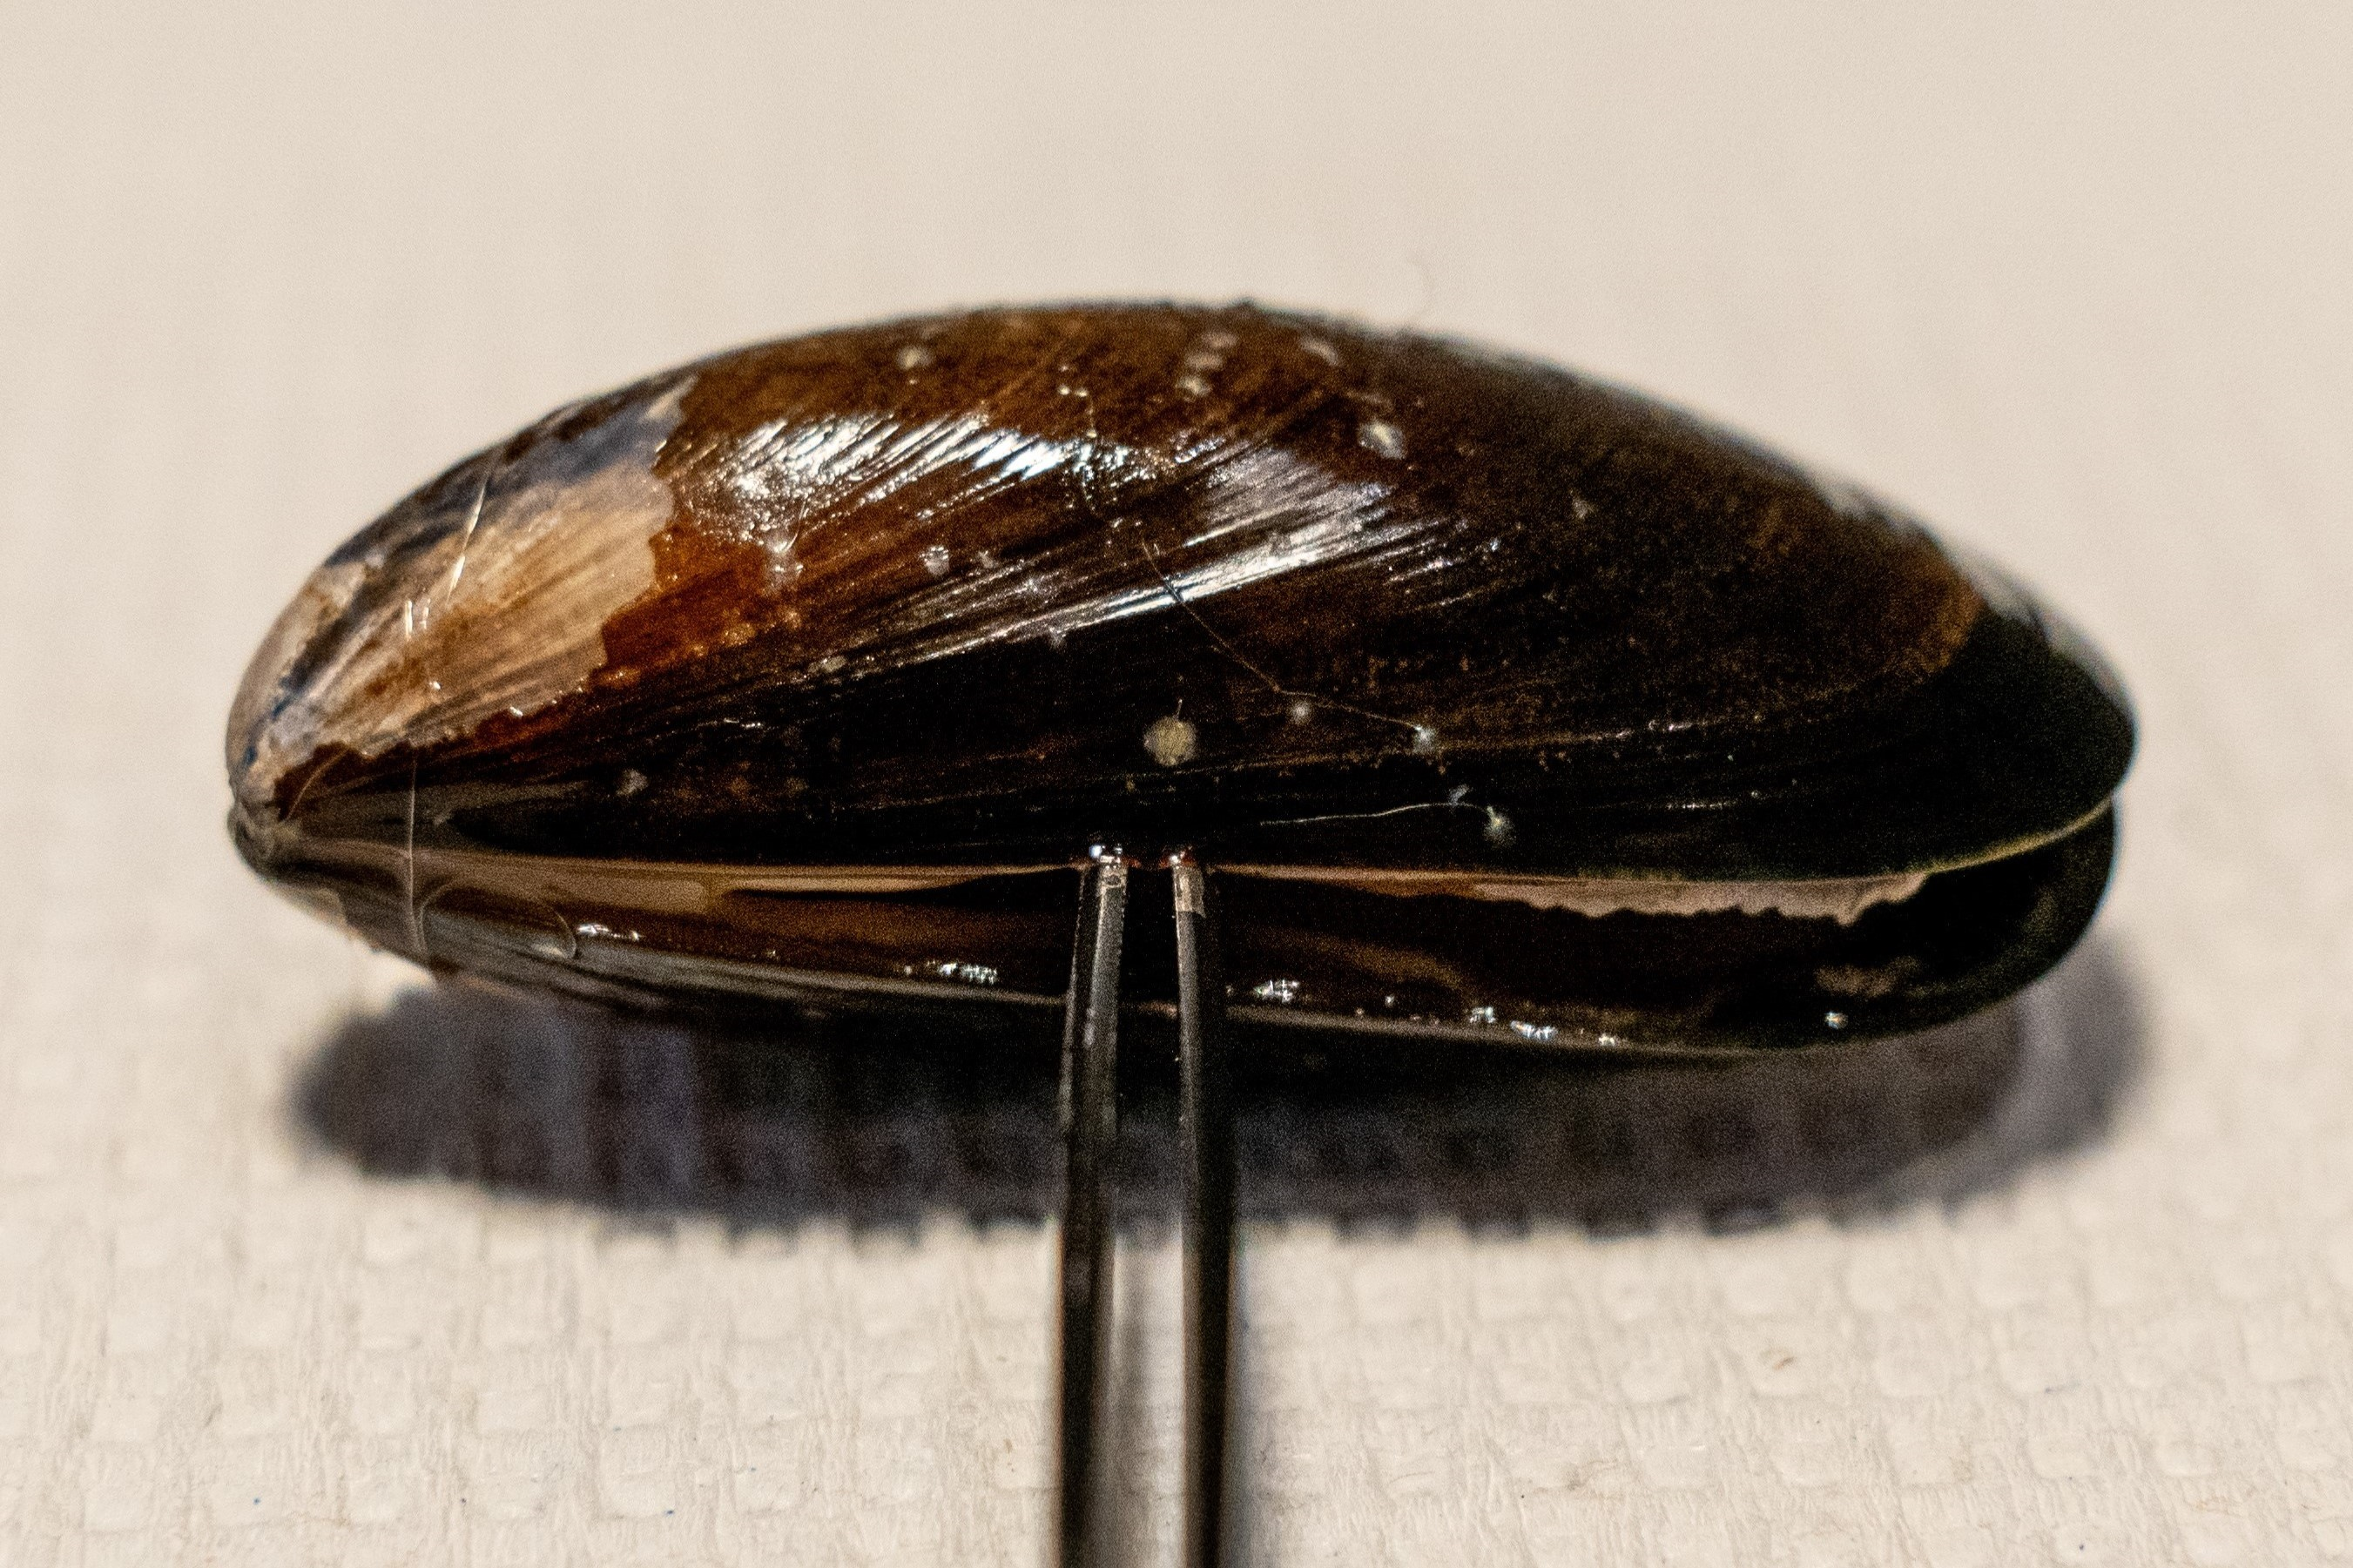
\includegraphics[width=\textwidth]{figures/Sampling technique/forceps square color.jpg}
        \caption{Placement of forceps between valves on the ventral side of the mussel.}
        \label{sfig:a}
    \end{subfigure}
    \hfill
    \begin{subfigure}[b]{.45\textwidth}
        \centering
        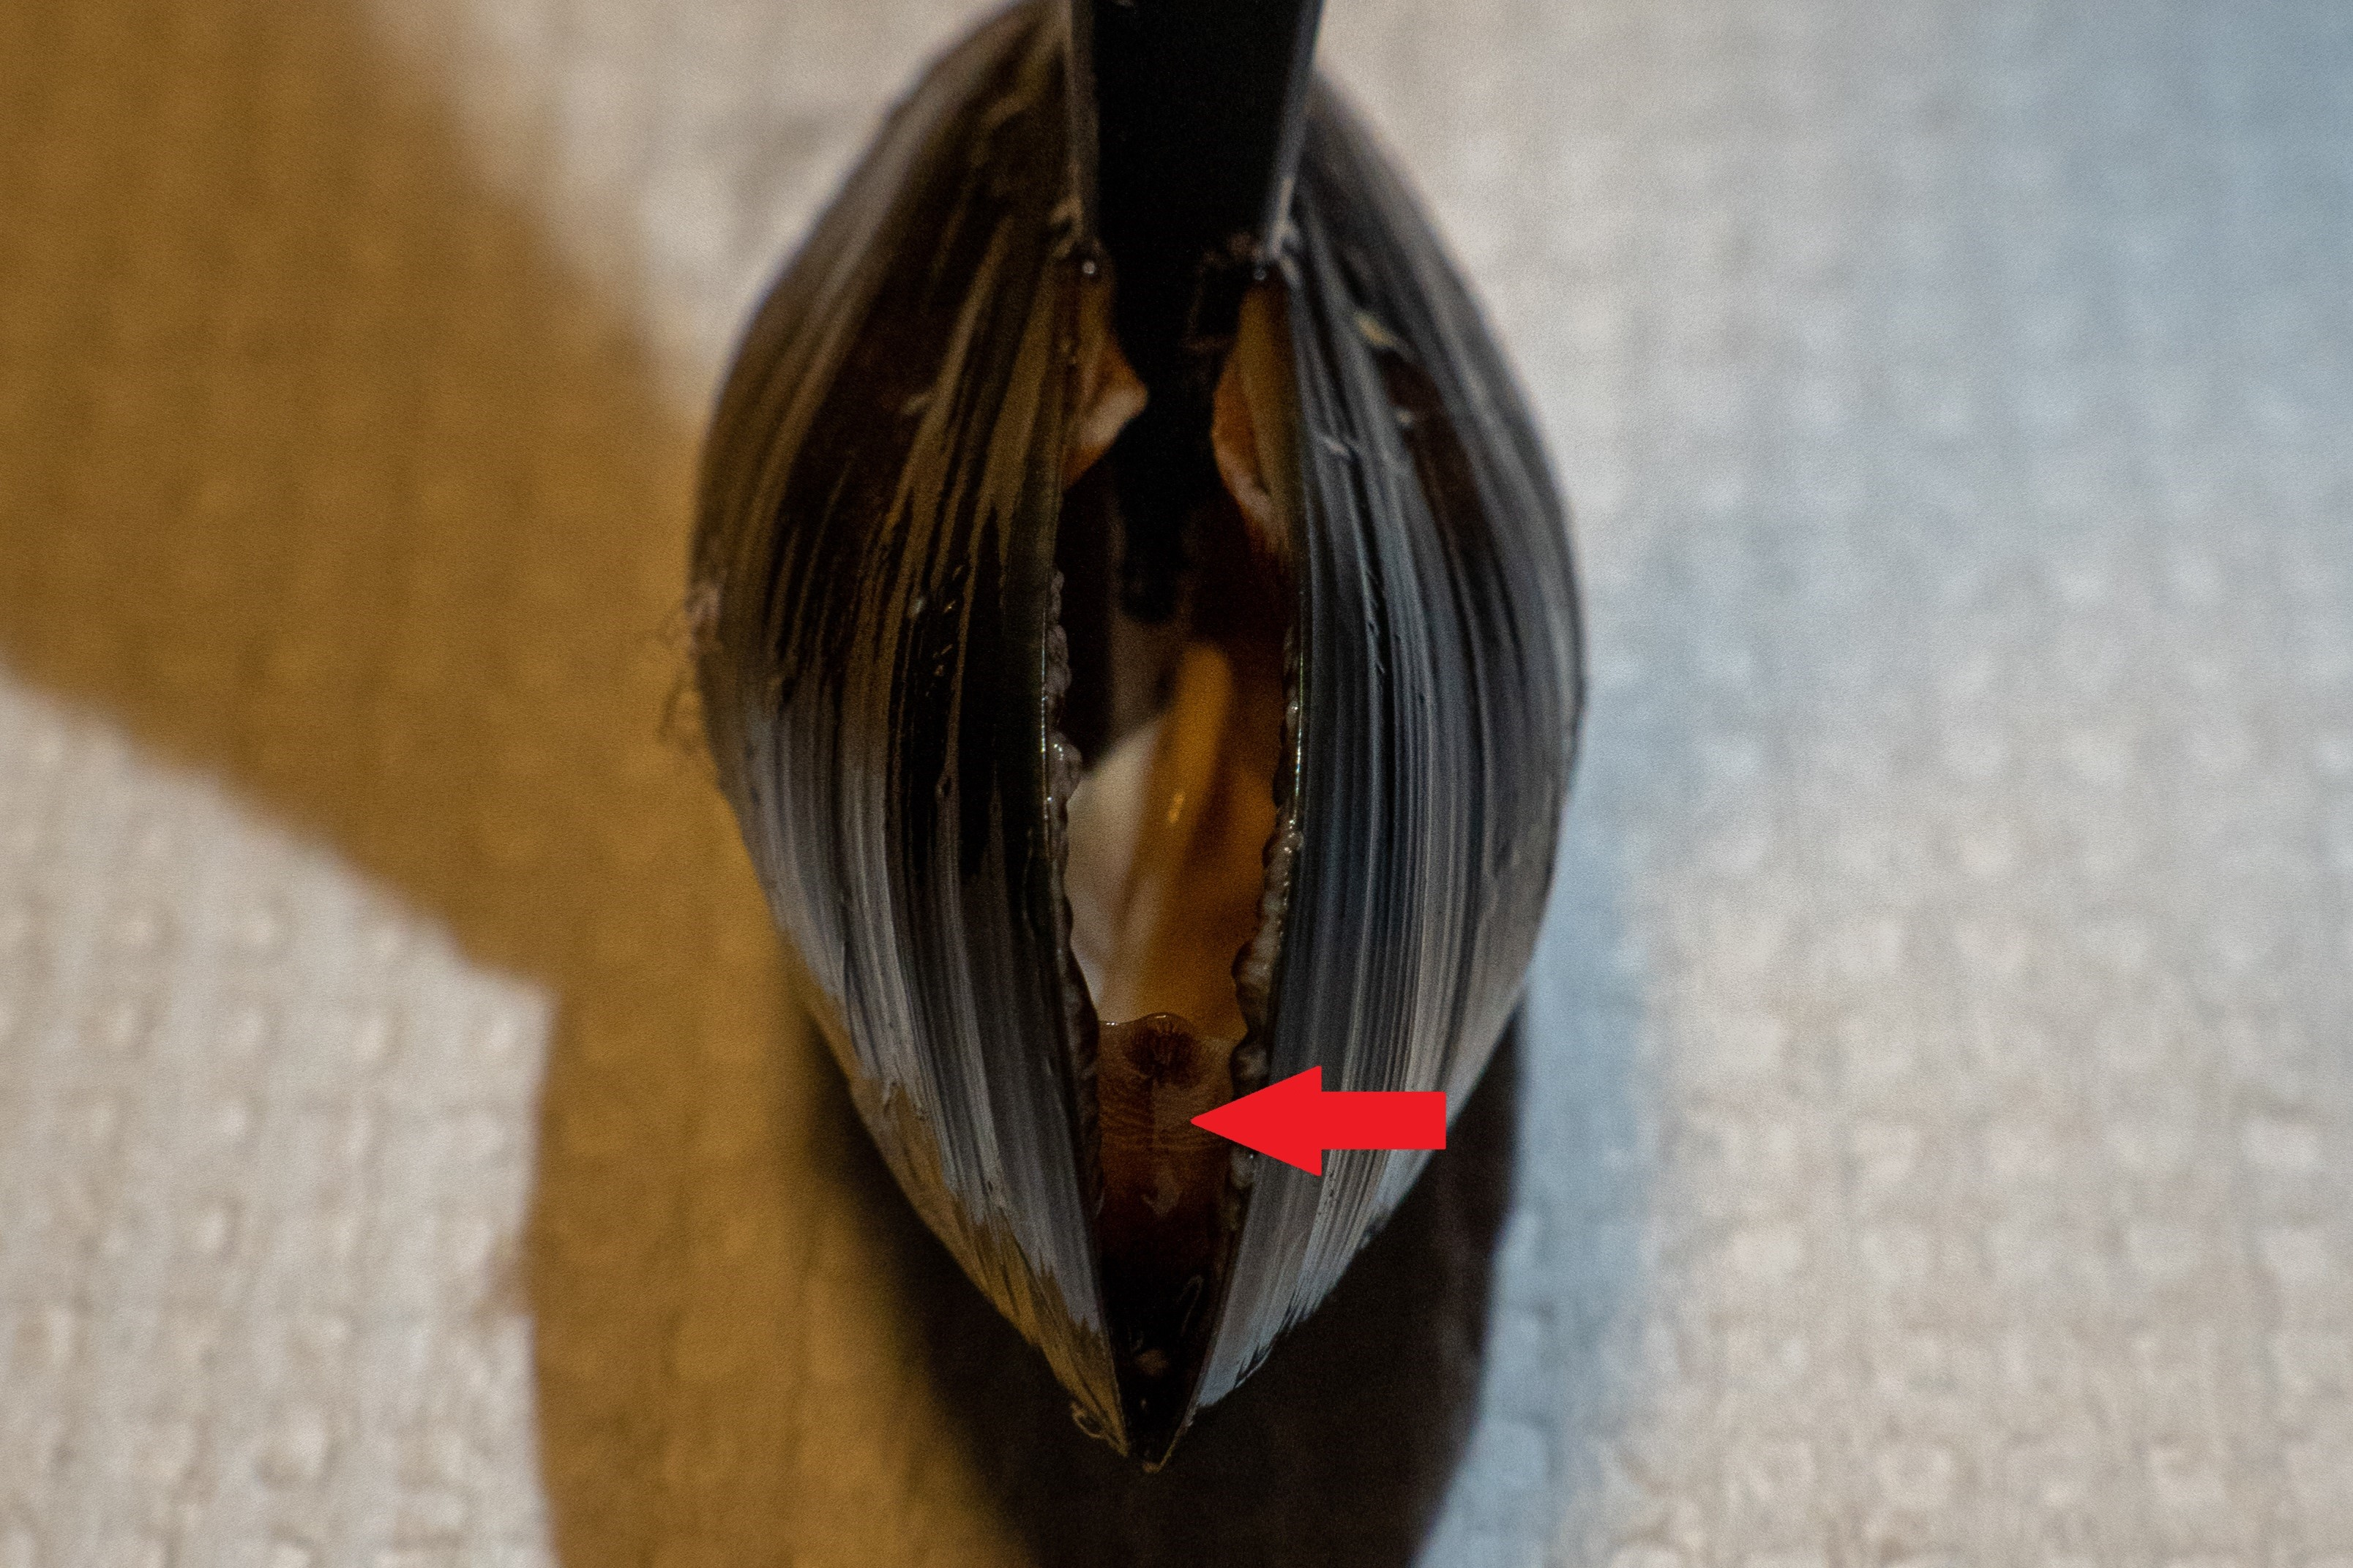
\includegraphics[width=\textwidth]{figures/Sampling technique/uncut color 3495.jpg}
        \caption{Posterior aspect of mussel with the connecting mantle intact (red arrow).}
        \label{sfig:b}
    \end{subfigure}
    \newline
    \begin{subfigure}[b]{.45\textwidth}
        \centering
        \includegraphics[width=\textwidth]{figures/Sampling technique/possible match.jpg}
        \caption{Mussel with the posterior adductor muscle (red arrow) clearly visible with the connecting mantle cut.}
        \label{sfig:c}
    \end{subfigure}
    \hfill
    \begin{subfigure}[b]{.45\textwidth}
        \centering
        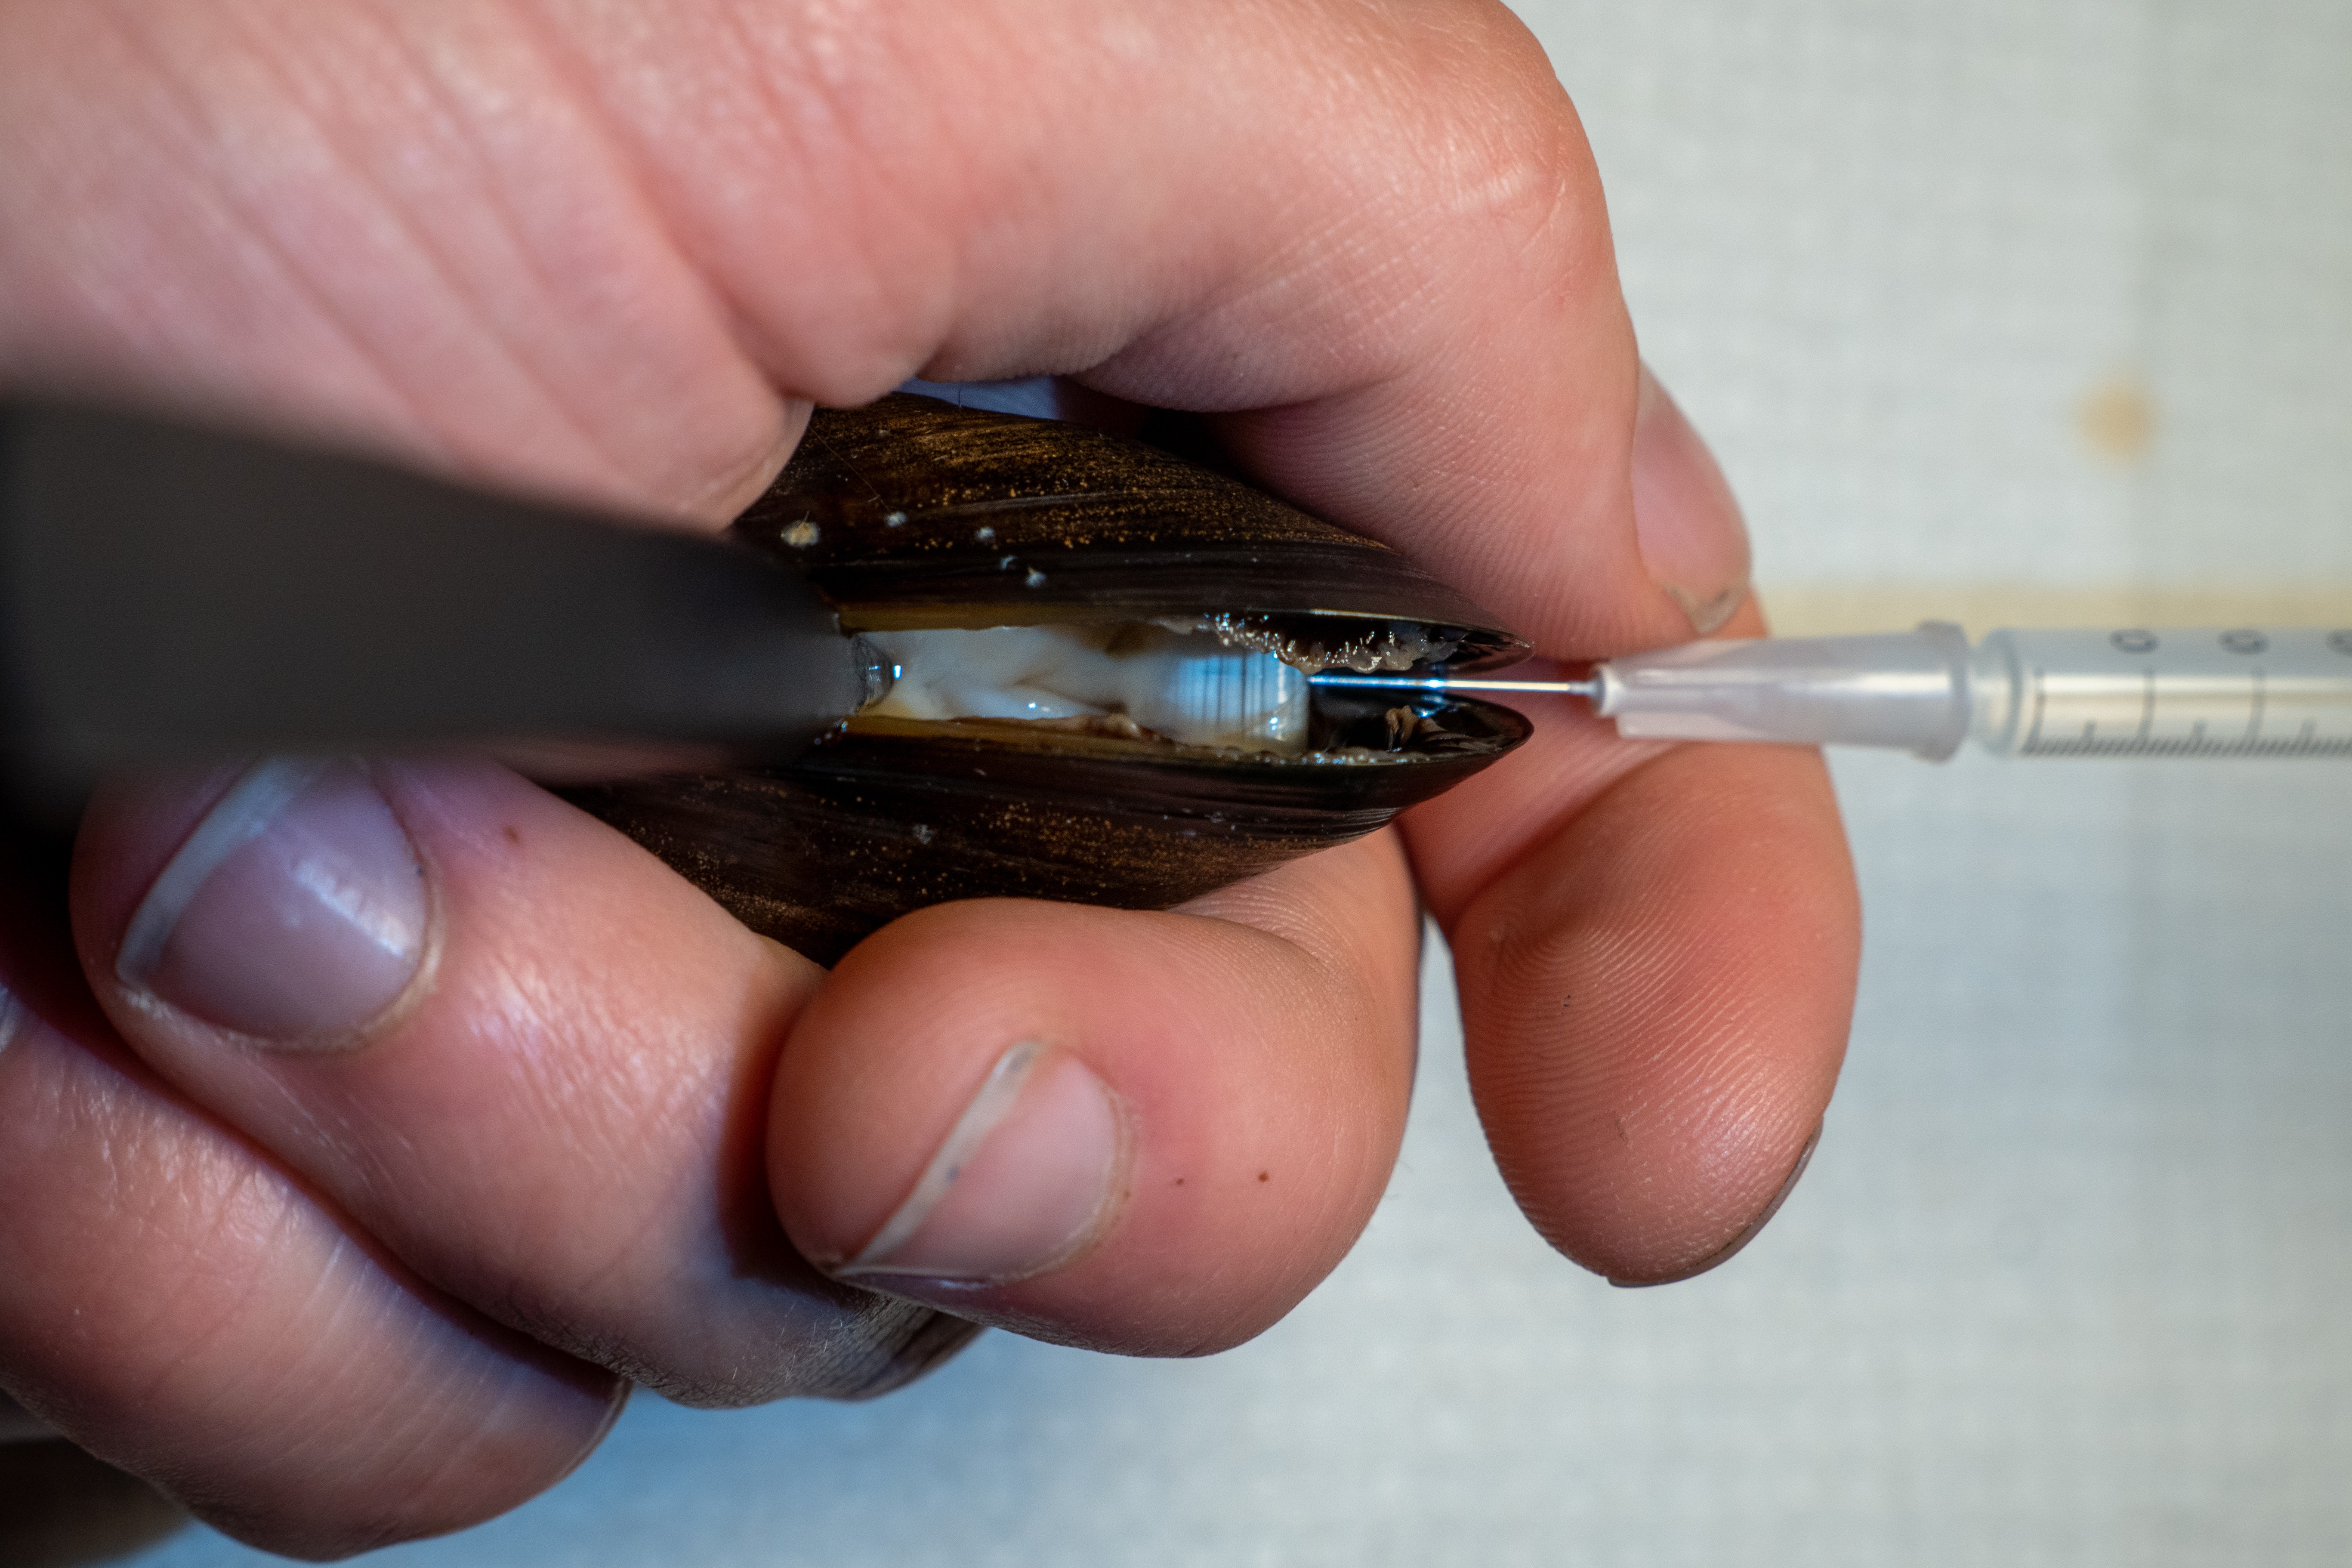
\includegraphics[width=\textwidth]{figures/Sampling technique/hands colors centered.jpg}
        \caption{The mussel grip and needle alignment employed, seen from the operators perspective.}
        \label{sfig:d}
    \end{subfigure}
    \caption{An illustration of the method employed to extract hemolymph from the posterior adductor muscle of M. edulis in order to avoid off-target withdrawal of pallial fluid or spermatozoa.}
    \label{fig:Hemolymph_sampling_illustration}
\end{figure}

For this work, 1.0 mL syringes equipped with sterile 23 gauge hypodermic needles were used. Hemolymph samples were gently withdrawn at an approximate rate of 1.0 mL/min, in order to prevent the negative pressure inside the muscle from drawing in pallial fluid between the muscle fibers. The mussels were placed in the palm of the operator's non-dominant arm, 3$^{rd}$-5$^{th}$ digits firmly gripping the mussel, 1$^{th}$ and 2$^{nd}$ digits keeping the syringe steady in the anteroposterior direction, while the dominant hand were used to withdraw the syringe plunger.

\subsection{Selection of haemocyte medium for flow cytometry assays}
The haemocytes of \emph{M. edulis} have a tendency to form aggregates upon mechanical stress, e.g. when the hemolymph is withdrawn through a thin syringe needle. Since accurate flow cytometric analyses rely on single-cell measurements, there was a need to minimize haemocyte aggregation during staining procedures, until the samples could by analyzed on the flow cytometer.

In the literature, several authors have dealt with this challenge by aspirating hemolymph samples directly into slightly acidic \acrshort{edta}-containing solutions buffered by citric acid (\cite{Söderhall1983, Bachere1988, LeFoll2010}). Since haemocyte aggregation is a Ca$^{2+}$-dependent process (\cite{Torreilles1999, Chen1995}), withdrawal of hemolymph into buffers containing divalent metal-ion chelators effectively slows the rate of haemocyte aggregation, allthough it does not inhibit aggregation completely (\cite{Chen1995}). Another frequently reported method is to dilute the hemolymph in cold filtered seawater (\acrshort{fsw}), while keeping the samples on ice prior to analysis. 

In search for the most effective method for this work, hemolymph samples were withdrawn into syringes pre-filled with a number of different "anticoagulant" or "antiaggregative" buffers (1:1) reported in the literature. The degree of aggregation was initially evaluated by inspecting hemolymph smears prepared following the method of Bolognesi and Fenech (2012) under 10x magnification. After preliminary testing, the most promising buffers encountered where the Modified Alsever's Solution (\acrshort{mas}, pH=7.0), and the similar Anticoagulant Buffer (\acrshort{acb}, pH=7.6) with \acrshort{edta} reported by \cite{Pipe1997}. To test their relative effects on haemocyte aggregation under the conditions intended for our flow cytometric analysis, a more specific comparison was needed to arrive at the most suitable buffer for this work.

\subsubsection{Haemocyte aggregation}
An experiment was seeded from the observation that \acrshort{fcm} singlet haemocyte counts tended to decrease over time from hemolymph withdrawal, and were based on the assumption that aggregation was the main driving factor. The proportion of aggregated haemocytes in a sample at a given time could therefore be retraced from the initial haemocyte count when performing several counts of the same sample over time. Since the difference in density between buffers would be negligible, the sedimentation rates would be independent of the haemocyte medium. Any observed differences would thus be caused by differences in the buffers' ability to inhibit aggregation.

500 \micro L hemolymph was withdrawn from 24 individual mussels into syringes prefilled with either 500 \micro L \acrshort{mas} (RT, n=8), \acrshort{acb} (RT, n=8) or cold Marine Physiological Saline Solution (\acrshort{mpss}, \SI{4}{\celsius}, n=8). Tris-buffered \acrshort{mpss} (pH=7.4) was used as a proxy for \acrshort{fsw}, such that pH and osmolarity could be controlled. The diluted hemolymph was transferred to 12$\times$75 mm polystyrene tubes and the initial haemocyte count were determined by acquiring 20 \micro L sample on the flow cytometer immediately thereafter. Each sample was run with identical acquisition and fluidics settings (see table \ref{tb:FCM_settings}), and the cells were gated on by a singlet inclusion gate (FSC-A vs. FSC-H) and a haemocyte gate (FSC-A v. SSC-A, see gating strategy). To account for any extra aggregation occurring from gentle mixing with flow cytometry reagents in the planned assay, each sample was gently pipetted up and down four times following the initial count. The second count were performed precisely 15 minutes later to mimic the incubation periods of our flow cytometry reagents. Three more singlet haemocyte counts where acquired from each sample at 30, 45 and 60 minutes post-withdrawal, to discern the buffers' ability to prevent aggregation during longer incubation periods. Samples withdrawn into \acrshort{mpss} were kept on ice between each singlet haemocyte count.

\subsubsection{Mixed logistic regression of the proportion of aggregated haemocytes}
The dataset consisted of 107 observations ($y_{ij}, t_{ij}$) from 24 individual mussels ($i$), $i = 1,...,n_{i}$, where $y_{ij}$ denotes the proportion of aggregated haemocytes from mussel $i$ at timepoint $t_{ij}$, $j = 1,...,n_{j}$, and $j$ represents repeated measurements of mussel $i$ at $t = (0, 60]$ minutes post-withdrawal. If we let $N_{t0}$ represent the initial haemocyte count of mussel $i$ at $t \approx 0$, the proportion of aggregated haemocyte at time $t_{ij}$ was calculated according to (\ref{eq: proportion_agg}):

\begin{equation}
    \label{eq: proportion_agg}
    y_{ij} = \dfrac{N_{t0} - N_{ij}}{(N_{t0} - N_{ij}) + N_{ij}} = \dfrac{N_{t0} - N_{ij}}{N_{t0}}
\end{equation}

\noindent where $N_{ij}$ denotes the hemocyte count of mussel $i$ at time $t_{ij}$.

The buffers' ability to inhibit haemocyte aggregation was tested statistically by mixed effects logistic regression, such that the within-individual correlation could be modelled as random effects to account for repeated measurements. The proportions were modelled as a function of log time, with buffer as a categorical explanatory variable. The mixed logistic regression model was fitted by maximum likelihood (Laplace approximation) using the \emph{glmer} function of the R package \emph{lme4} (\cite{lme4}), with a "binomial" error distribution and "logit" link function, as shown in Code listing 3.1. However, instead fitting the model with the calculated proportions ($y_{ij}$), the response variable was formatted as a two-column matrix of aggregated and singlet haemocyte counts, for the response to be weighted by $N_{t0}$. The format of the response matrix is shown in (\ref{eq:agg_free_matrix}).

\begin{lstlisting}[language=R, caption = {The R source code run to fit the logistic proportion aggregation model.}]
model = glmer(data = df, formula = y ~ log(t)*Buffer + (log(t)|ID),
                 family = binomial(link = "logit"))
\end{lstlisting}

\begin{equation}
    \label{eq:agg_free_matrix}
    y_{i} := \begin{pmatrix}
     M_{1} \\
     \vdots \\
     M_{i} \\
     \vdots \\
     M_{n_{i}} \\
    \end{pmatrix}
    , \; \; \; \; M_{i} \: = \:
    \begin{pmatrix}
      N_{t0} - N_{i1}     &  N_{t0} \\
      \vdots              &  \vdots \\
      N_{t0} - N_{ij}     &  N_{t0} \\
      \vdots              & \vdots \\
      N_{t0} - N_{in_{j}} &  N_{t0} \\      
    \end{pmatrix}
\end{equation}

The factor levels of the categorical explanatory variable was defined as dummy variables (see equation \ref{eq:dummy_variables}), where the \acrshort{mpss} buffer was set as reference level. Thus, the fitted proportion of aggregated haemocytes ($y_{ij}$) in a sample from mussel \emph{i} = [1, 24] at time $t_{ij}$, \emph{j} = (0, 60], can be written out on \emph{logit} scale as in (\ref{eq:logit}), where $\alpha_{1} \: + \: \beta_{1}log(t_{ij})$ is the linear predictor of the reference level, $\alpha_{2}$ and $\alpha_{3}$ represents the difference in y-intercept for the \acrshort{acb} and \acrshort{mas} buffers, $\beta_{2}$ and $\beta_{3}$ represents the differences in slopes, while $\gamma_{0i}$ and $\gamma_{1i}$ represents the individual-specific deviation from the population intercept and slope, respectively. The linear predictors relate to the log proportions according to (\ref{eq:linear_predictors}), where the dummy variables $D_{2}$ and $D_{3}$ have been solved according to (\ref{eq:dummy_variables}).

\begin{equation}
    \label{eq:dummy_variables}
D_{2} =\begin{cases}
      1, & \text{ACB}\\
      0, & \text{not ACB},
    \end{cases}
    \quad
D_{3} =\begin{cases}
      1, & \text{MAS}\\
      0, & \text{not MAS}
    \end{cases}
\end{equation}

\begin{equation}
\label{eq:logit}
y_{ij} = \dfrac{1}{1 + e^{-(\alpha_{1} \: + \: \beta_{1} log(t_{ij}) \: + \: D_{2}(\alpha_{2} + \beta_{2}log(t_{ij})) \: + \:  D_{3}(\alpha_{3} + \beta_{3}log(t_{ij})) \: + \: \gamma_{0i} \: + \: \gamma_{1i}log(t_{ij}))}}
\end{equation}

\begin{equation}
    \label{eq:linear_predictors}
    \resizebox{\linewidth}{!}{$
    log\dfrac{P(y_{ij} = 1 \mid t_{ij}, \gamma_{0i}, \gamma_{1i})}{P(y_{ij} = 0 \mid t_{ij}, \gamma_{0i}, \gamma_{1i})} = \begin{cases}
        \alpha_{1} + \gamma_{0i} + (\beta_{1} + \gamma_{1i})log(t_{ij}), & i \: \text{in MPSS group}, \\
        \alpha_{1} + \alpha_{2} + \gamma_{0i} + (\beta_{1} + \beta_{2} + \gamma_{1i})log(t_{ij}), & i \: \text{in ACB group}, \\
        \alpha_{1} + \alpha_{3} + \gamma_{0i} + (\beta_{1} + \beta_{3} + \gamma_{1i})log(t_{ij}), & i \: \text{in MAS group} \\
    \end{cases}
    $}
\end{equation}

Since generalized linear mixed models (\acrshort{glmms}) do not allow for a marginal interpretation of coefficients, the group-averaged proportions of aggregated haemocytes after 15 minutes post-withdrawal were compared by conventional two-sample t-tests. This timepoint was chosen specifically, since the required incubation with flow cytometric viability dyes would most likely not surpass 15 minutes (\cite{Nescerecka2016}).

\subsubsection{EDTA cytotoxicity}
One of the aims of this project was to count the number of necrotic haemocytes present in the hemolymph of \emph{M. edulis} by means of flow cytometry. Since the mussels were to be exposed to \ce{TiO2} and Ag nanoparticles \emph{in vivo} for 21 days, the targeted endpoint would be the number of necrotic haemocytes circulating in their hemolymph at the timepoint just before hemolymph extraction on day 22. Any acute effects on viability arising from the hemolymph extraction itself, or during incubation with the viability stains between extraction and count, would serve to obscure the potential \emph{in vivo} effect of the nanoparticles. Since high concentrations of \acrshort{edta} has been reported to impair hemocyte viability (\cite{Grandiosa2018, Burkhard2009}), a direct comparison of \acrshort{mas} and \acrshort{acb} with regards to acute effects on viability was required to ensure their suitability as anticoagulants for flow cytometric assays, i.e., to make sure that the buffers themselves did not interfere with the targeted endpoint. 

To test wether the \acrshort{edta}-containing buffers had any effects on haemocyte viability in the 15 minute time window required for staining, 500 \micro L hemolymph was withdrawn from 24 individual mussels into syringes prefilled with either 500 \micro L \acrshort{mas} (n=8) or \acrshort{acb} (n=8). Hemolymph from the last eight mussels were withdrawn into cold \acrshort{mpss} and kept on ice as negative \acrshort{edta}-controls. The diluted hemolymph were transferred to 12$\times$75 mm polystyrene tubes, were they were stored for 15 minutes before staining 300 \micro L subsamples with 1.0 \micro L \acrshort{calceinam} (50 \micro M) and 3.6 \micro L TO-PRO$^{TM}$-3 Iodide (100 \micro M) dissolved in \acrshort{dmso}. The samples were incubated in darkness for 15 minutes, before 10.000 haemocyte events were recorded on the flow cytometer without washing.

488 nm-exited green fluorescence from hydrolyzed Calcein were recorded on the FL1 detector with a 533/15 nm filter, while the 640 nm-exited far red fluorescence from DNA-bound TO-PRO$^{TM}$-3 Iodide were recorded on the FL4 detector with a 675/25 nm filter. The events were gated according to the gating strategy in figure (\ref{fig:TP3_Calcein_gating_strat}), obtaining counts of live (Calcein$^{+}$ToPro3$^{-}$), necrotic (Calcein$^{-}$ToPro3$^{+}$) and doubly stained (Calcein$^{+}$ToPro3$^{+}$) haemocytes, as well as non-cellular particles (Calcein$^{-}$ToPro3$^{-}$) and a total count. In this particular experiment the doubly stained haemocytes were counted as necrotic, as newly damaged or lysed haemocytes might still retain a degree of non-specific esterase activity. Hence, the percentage of necrotic haemocytes were calculated according to equation \ref{eq:necrotic hemocytes}.

\begin{equation}
    \label{eq:necrotic hemocytes}
    \text{Necrotic haemocytes (\%)} = \dfrac{n_{Calcein^{-}ToPro3^{+}} + n_{Calcein^{+}ToPro3^{+}}}{n_{total} - n_{Calcein^{-}ToPro3^{-}}} \times 100
\end{equation}

The 700 \micro L remaining of each hemolymph sample were stored for another 2 and 20 hours, and the same staining and flow cytometric measurements were repeated at these timepoints. Because of considerable aggregation and sedimentation of haemocytes in \acrshort{mpss} after 2 and 20 hours, and those kept in \acrshort{mas} and \acrshort{acb} for 20 hours, the haemocytes in these samples were resuspended with a wide bore pipette before the second and third rounds of staining.

\subsubsection{Cytotoxicity of acidic haemocyte medium pH}
The Modified Alsever's Solution (MAS) is an anticoagulant medium developed to inhibit aggregation among invertebrate haemocytes, while maintaining cell viability (\cite{Bachere1988}). It contains D-Glucose (20.5 g/L), \ce{NaCl} (21.95 g/L), \ce{Na2EDTA}$\cdot$\ce{2H2O} (4.3 g/L), and is buffered by Citric acid (8.0 g/L) and tri-basic citric acid (0.55 g/L). The citric acid maintains an effective buffer range of 6.1$\pm{0.2}$, and the acidic pH is thought to somehow contribute to the anticoagulant effect (\cite{Söderhall1983, Renwartz1990}). The pH can be raised to 7.0, but the buffer capacity at this range is practically non-existent. Since pH-adjusted MAS (pH = 7.0) had proven as an effective tool for reducing haemocyte aggregation, there were obvious reasons for testing if it could be used in it's intended pH-range.

However, since the pH of non-adjusted MAS (\acrshort{namas}, pH = 6.1) is considerably lower than that of seawater and haemolymph, the acidic environment could potentially induce apoptosis and interfere with the endpoints of the planned flow cytometric Apo-15/TO-PRO-3 Iodide apoptosis assay (\cite{Wang2016}). To test wether the effective pH of naMAS:haemolymph (1:1) had any measurable effect on the percentage of early apoptotic (Apo15$^{+}$/ToPro3$^{-}$) and necrotic (Apo15$^{+}$/ToPro3$^{+}$) haemocytes; haemolymph from 36 mussels were withdrawn into an equal volume of naMAS (n=18) and ACB (n=18). The slightly alkaline pH of ACB (pH = 7.6) is adapted to reflect that of \emph{M. edulis} haemolymph (\cite{Pipe1997, Mangan2019}), and was therefore used as a negative control for acidic buffer pH. The haemocytes were incubated in the media for 15 minutes prior to staining with Apo-15 (560 nM) and TO-PRO$^{TM}$-3 Iodide (1.2 \micro M). After incubating for another 15 minutes, 10.000 events were acquired from each sample on the flow cytometer.

\subsubsection{Haemocyte viability: Statistical analysis}
The mean percentage of necrotic haemocytes in \acrshort{mpss}, \acrshort{acb} and \acrshort{mas} were compared by one-tailed two-sample t-tests at the three different timepoints. Since the group variances ($s^{2}$) differed by more than a factor of 2 at the last timepoint, these comparisons were bade by Welch two-sample t-tests. Paired t-tests were used to assess wether the percentages of necrotic haemocytes increased with incubation time within each group. The mean percentage of early and late apoptotic haemocytes in naMAS and ACB were compared by Welch two-sample t-tests.

\subsection{Cytologic characterization of haemocyte subpopulations}
\label{subsection:morph}
For the purpose of characterizing and imaging the different haemocyte cell types of \emph{M. edulis} in a non-spread state, samples were withdrawn into an equal volume of ice-cold \acrshort{mpss} and transferred directly onto glass slides. The glass slides were kept in a humid chamber for up to 5 minutes before cells were fixed in ice cold methanol (5$\times$ 1 sec dips). This assured haemocyte attachment, but circumvented the profound morphological changes accompanied by the haemocytes’ process of spreading. Slides were stained with the Hemacolor\textsuperscript{\textregistered} kit according to the manufacturer’s recommendations, air dried, mounted with Eukitt\textsuperscript{\textregistered} and coverslipped. Stained haemocytes were examined and imaged under brightfield illumination on a Nikon Eclipse 90i upright microscope with a 100$\times$/1.40 oil immersion objective and a Nikon DS-Fi1 microscope camera. Haemocyte morphology was characterized on the basis of cytoplasmic staining, granularity (granule size, abundance and staining affinities), nuclear:cytoplasmic (N:C) ratio, cell diameters and shape. 

\subsection{Determination of cell diameters}
\label{subsection:CytCar}
To establish wether haemocyte subpopulations differed with regard to size across a larger population of adult mussels, the cell diameters of 100 haemocytes were ascertained in haemolymph smears from 20 individual mussels (n=2000). Since the rate and degree of haemocyte spreading could be inherently different among cell types, all spreading was effectively impeded by collecting haemolymph samples into an equal volume of 5\% formaldehyde in \acrshort{mpss}. The fixation was continued for one hour in suspension, before cells were pelleted by centrifugation (250G, 15 min, \SI{10}{\celsius}) and resuspended in 100 \micro L 0.75 \% eosin in Sorensen Buffer. After staining for 5 minutes, 1 mL 3\% Wright’s-Giemsa was added and the staining was continued for an additional 15 minutes. Stained haemocytes were pelleted by centrifugation (180G, 12 min, \SI{10}{\celsius}), resuspended in 100-200 \micro L Sorensen Buffer and transferred onto glass slides. The slides were air-dried in a fume hood until the smears were completely dry and transparent, before they were mounted with Eukitt\textsuperscript{\textregistered} and coverslipped.

The slides were placed on the stage of a Nikon Eclipse 80i upright microscope, and 10-20 microscopic fields from each smear was photographed under DIC illumination with a $\times$60 oil immersion objective. Cell diameter measurements were performed digitally with ImageJ (NIH, Bethesda, Maryland, US), using the \emph{Straight line tool} of this image processing software. The actual size of the magnified haemocytes were determined by calibrating the software's pixel/\micro m scale with a stage micrometer calibration slide (Leitz Wetzlar, Buffalo, DE), photographed with the same equipment and image resolution as the haemolymph smears. When haemocyte outlines deviated from an approximate spherical shape, the diameter was estimated as the average length of the long and short axes, after Burkhard et al. (2009). The measurements were performed as differential counts, such that the number of measurements of each cell type reflected their average relative proportions (\%) across all 20 mussels.

\subsection{Flow cytometric characterization of haemocyte subpopulations by light-scatter measurements}
Throughout the methodological and experimental work that was done in relation to this project, more than 500 adult mussels were samples for haemolymph, and the majority of these samples were run as suspensions of living haemocytes on the BD Accuri C6 Plus Flow Cytometer. The purposes of these measurements varied to a large extent, but the samples were invariably examined as bivariate plots of Forward Scatter (FSC) vs. Side Scatter light (\acrshort{ssc}) at some point in the analyses. These investigations revealed a substantial amount of variation between individual mussels in terms of the relative proportions of their haemocyte subpopulations and their separation according to FSC vs. \acrshort{ssc}.

A quantitative flow cytometric characterization of the haemocyte subpopulations of \emph{M. edulis} can be found in Le Foll et al. (2010), who utilized a flow cytometer equipped with a Coulter-type electronic cell-volume analyzer to characterize haemocytes in terms of cell diameter (\micro M) vs. \acrshort{ssc}. Instead of repeating this endeavor with relative units of \acrshort{fsc}, the scope of the current flow cytometric characterization was to present the typical light-scatter profile of adult mussels, while representing the observed variation with a few examples of extreme observations. The haemolymph samples were withdrawn into an equal volume of \acrshort{acb} according to the technique described in section \ref{subsection:haemolymph sampling technique}, and were analyzed on the flow cytometer directly thereafter.

\subsection{Relating cytologically defined cell types to light-scatter profiles}
As mentioned in theory section \ref{subsection:haemocyte_classification}, the use of flow cytometers with cell sorting capabilities can simplify the process of verifying a classification derived from flow cytometric measurements. However, since the BD Accuri C6 Plus is not equipped with a cell sorter, other measures were taken to relate the cytologically defined cell types in section \ref{subsection:Results_cytchar} to the subpopulations defined by flow cytometry in section \ref{subsection:Results_FlowChar}.

Cell sorters facilitate visual inspections of cells with known measured characteristics following a flow cytometric measurement. This workflow can be reversed if the cells are sorted by other means prior to flow cytometric acquisition. This section describes how pools of Giemsa-stained haemocytes were separated by isopycnic centrifugation, and how the isolated cell fractions were characterized by flow cytometry and microscopy thereafter. Subsequently, the flow cytometric "separation" of haemocytes according to eosin fluorescence is described.

\subsubsection{Isopycnic centrifugation}
Formaldehyde-fixed haemocytes were separated on discontinuous Percoll gradients according to the protocol by Friebel and Renwrantz (1995), with minor modifications. The separation was performed in duplicate with pooled haemocytes from a total of six adult mussels (shell length 58$\pm{12}$ mm). For both gradients, the haemolymph of three individual mussels (1.5-2.0 mL/mussel) were withdrawn into an equal volume of 5\% formaldehyde in \acrshort{mpss}, wherein the haemocytes were fixed for one hour after pooling. The fixed haemocytes were stained with 0.75 \% Eosin and 3 \% Giemsa according to the procedure in section~\ref{subsection:CytCar}. After pelleting, stained haemocytes were resuspended in Tris-Buffered Saline (\acrshort{tbs}, 900 mOsm) to an approximate concentration of $9\times10^{6}$ cells/mL, before layering 2 mL suspension on top of both gradients. Discontinuous Percoll gradients consisted of 15\%, 33\%, 38\%, 43\% and 90\% Percoll stock in \acrshort{tbs} (vol/vol), and were constructed by carefully layering 2 mL of each Percoll concentration in 15 mL Falcon centrifuge tubes with conical bottoms (Corning, New York, US).

The centrifugation was started at 120G for 10 minutes (\SI{4}{\celsius}), followed by 40 minutes at 2500G. An Eppendorf 5804 R benchtop centrifuge equipped with an A-4-44 swing-bucket rotor was employed for the separation, with the brake ramp set to 1. The separated cell fractions were collected into syringes by puncturing the tubes below the gradient interfaces with 23G hypodermic needles. According to a protocol by Bachére and Grizel (1988), the Percoll was eliminated from the 43/90\% and 38/43\% fractions by two consecutive dilutions in \acrshort{tbs} (1:7) and a 10\% sucrose cushions (1:1) before centrifugation (800G, 15 min, \SI{4}{\celsius}). Haemocytes collected from the 15/33\% interface were centrifuged directly after a seven-fold dilution in \acrshort{tbs} (800G, 15 min, \SI{4}{\celsius}).

The pelleted cell fractions were resuspended in Sorensen buffer and divided into two aliquots; one aliquot were used to prepare smears according to the procedure in section \ref{subsection:CytCar}, while the remaining aliquots were further diluted in 1 mL Sorensen buffer for flow cytometric characterization. A total of 10.000 events were acquired from each cell fraction on the flow cytometer (36 \micro L flow rate, 16 \micro m core size), in addition to 30.000 events from both pools that were set aside prior to centrifugation. The relative proportion (\%) of cell types in each fraction were ascertained by performing 1000-cell differential counts. 

\subsubsection{Identification of eosinophilic granulocytes by eosin fluorescence}
Since Eosin is fluorescent in the green/yellow spectrum (\acrshort{exmax}/\acrshort{emmax}: 517/543 nm) (\cite{Koegle2020}), blue laser-exited fluorescence from this anionic dye can be collected on the FL1 detector (518-548 nm) of the BD Accuri C6 Plus flow cytometer (BD Biosciences, California, US). If the haemocytes of \emph{M. edulis} are permeabilized and stained with eosin prior to flow cytometric analysis, the fluorescent signal from Eosin can in theory be used to identify eosinophilic granulocytes on \acrshort{fsc} vs. \acrshort{ssc} dotplots by backgating.

This approach was attempted by Le Foll an colleagues (2010), who detached spread haemocytes stained by eosin with an \acrshort{edta}/trypsin solution followed by flow cytometric analysis. As noted in the theory section (\ref{subsection:haemocyte_classification}), their results indicated that eosin$^{bright}$ events corresponded to haemocytes with high \acrshort{ssc} and \acrshort{fsc}-values. However, this exact methodology did not result in well-defined eosin$^{bright}$ and eosin$^{dim}$ peaks, such that the lower bound of their electronic eosin$^{bright}$ gate had to be drawn more or less arbitrarily. It could therefore not be used to pinpoint the exact border between the cell types when the subpopulations were overlapping with respect to SSC. 

Since their results were never verified by microscopy, their eosinophilic granulocyte gate cannot implemented in this work without further redo. An attempted was therefore made to optimize the basic approach of Le Foll et al. (2010), and to verify the results by light microscopy. This process involved exploring different fixatives, methods of fixation, eosin staining solutions and the duration of both fixation and staining - in order to achieve a practically applicable resolution between eosinophilic granulocytes and the rest of the haemocytes. 

After fixing haemocytes in suspension with concentrated methanol, Carnoy’s fixative and 5\% formaldehyde in MPSS, the only smears without high degrees of unspecific eosin staining were those fixed in 5\% formaldehyde. To reduce the passive diffusion of eosin into non-target cells, 5\% formaldehyde in \acrshort{mpss} was selected for further testing - being the softest fixative of the three. By diluting the eosin component of the Hemacolor\textsuperscript{\textregistered} kit in Sorensen buffer, a set of diluted staining solutions with 0.25\%, 0.5\%, 0.75\%, 1.0\%, 1.5\%, 3\%, 5\%, and 8\% eosin (vol/vol) were prepared. Samples that were stained with the 0.5\% eosin solution (5 min) separated into two distinct populations of events according to log eosin fluorescence. When the eosin$^{bright}$ population was back-gated to FSC vs. SSC dotplots, the presumed light scatter profile of the eosinophilic granulocytes were obtained.

The test wether the eosin$^{bright}$ (\%) events from flow cytometric analyses corresponded the eosinophilic granulocytes exclusively, this methodology was combined with microscopic 1000-cell differential counts, where the percentage of eosinophilic granulocytes was determined relative to the basophilic haemocytes. Haemolymph samples from 10 individual mussels were withdrawn into an equal volume of 5\% formaldehyde in MPSS and stained for 1 hour. The fixed cells were pelleted by centrifugation (180G, 12 min, \SI{20}{\celsius}) and resuspended in 0.5\% eosin in Sorensen buffer. The suspensions were divided into two aliquots, where one was pelleted and resuspended in 1 mL ACB after 5 minutes of staining, while the other was used to prepare Giemsa-smears according to the method described in section \ref{subsection:CytCar}. Samples in ACB were analyzed on the flow cytometer, while the corresponding Giemsa smears were used for differential counts. The correlation between eosin$^{bright}$ events (\%) and the percentage of eosinophilic granulocytes in the samples was tested by simple linear regression, in addition to calculating the mean percent error (\acrshort{mpe}) relative to the differential counts.

\subsection{Flow cytometric differential haemocyte count}
Since MRP-mediated efflux of \acrshort{calceinam} is shown to be higher in eosinophilic granulocytes, the differential accumulation of hydrolyzed calcein could possibly serve as a discriminator in flow cytometric differential haemocyte counts in \emph{M. edulis}. To test the applicability of calcein florescence (518-548 nm) in combination with SSC measurements for this purpose, the haemolymph of 22 untreated adult mussels were sampled for parallel flow cytometric analyses and microscopic differential haemocyte counts, i.e., twice subsequently.

\subsubsection{Characterization of haemocytes according calcein efflux and SSC}
The first round of samples were withdrawn into an equal volume of ACB and stained with 50 nM \acrshort{calceinam} for 15 minutes prior to recording 10.000 events on the flow cytometer. The flow cytometry data was analyzed as bivariate plots of (1) calcein fluorescence vs. log SSC and (2) FSC vs. log SSC, and the identity of the resultant subpopulations were compared by backgating. The subsequent samples were withdrawn into an equal volume of 5\% formaldehyde in MPSS and fixed for 1 hour. The fixed haemocytes were pelleted by centrifugation (250G, 15 min, \SI{10}{\celsius}) and resuspended in 3\% Giemsa to prepare smears according to the method described in section \ref{subsection:CytCar}. The Giemsa smears were used for 1000-cell differential haemocyte counts - where the percentage of eosinophilic granulocytes, basophilic granulocytes and small blast-like basophils were determined under 40x magnification on a Nikon Ni-U microscope (Nikon Corp, Tokyo, JP).

\subsubsection{Gating strategy and validation}
The three subpopulations that were distinguihable according to log calcein fluorescence vs. log SSC were gated according to the regions presented in Figure \ref{fig:DHC_gatestrat}. As these subpopulations corresponded to cluster 1-3 in bivariate plots of FSC vs. log SSC (see section \ref{subsection:calcein_SSC_char}), cluster 1, 2 and 3 were gated indirectly by substituting FSC for log calcein fluorescence in the flow cytometric differential haemocyte count. The percentages of events in cluster 1, 2 and 3 were calculated from the total number of singlet events recorded per sample (see Figure \ref{fig:DHC_gatestrat}A). On average, there were 9865$\pm{112}$ events/sample. These percentages were in turn used as estimates for the percentage of small blast-like basophils (cluster 1), basophilic granulocytes (cluster 2) and eosinophilic granulocytes (cluster 3) in each sample, respectively. The correlation between the estimated percentages and the microscopic counts were analyzed by simple linear regression for each cell type individually. Moreover, by calculating the mean percent error (\acrshort{mpe}) of the flow cytometric estimates relative to the microscopic counts, the accuracy of the method was evaluated. Two of the samples did not form three defined subpopulations according to log calcein fluorescence, and were excluded from the analysis.

\subsection{Scoring of necrotic haemocytes by flow cytometry}
To discriminate between viable and necrotic haemocytes by flow cytometry, a two-color fluorescence assay with the cell-permeant probe Calcein acetoxymethyl and the non-permeant \acrshort{dsdna}-binding dye TO-PRO$^{TM}$-3 Iodide (Molecular Probes, Eugene, OR) was chosen. This combination of probes was primarily selected for two reasons: (1) it enables simultaneous measurement of intracellular esterase activity and plasma membrane integrity - two recognized parameters of cell viability and (2) there is virtually no fluorescent spillover between the probes, such that the uncompensated raw data can be applied directly. Moreover, a complementary double staining methodology like this allows for discrimination between haemocytes and non-cellular particles. Since cells with intact plasma membranes retain esterase activity, double negative events (Calcein$^{-}$ ToPro3$^{-}$) of cellular proportions  must represent particles or cellular debris, since they do not contain \acrshort{dsdna} (ToPro3$^{-}$). 

Since Calcein AM is commonly used in the LIVE/DEAD\textsuperscript{\textregistered} Viability/Cytotoxicity Kit for mammalian cells (Molecular Probes, Eugene, OR), the staining protocol of this kit was used as a guide for obtaining an adequate fluorescent signal from hydrolyzed Calcein on the FL1 detector (518-548 nm). The manufacturer's recommendation of 50 nM Calcein AM mL$^{-1}$ cell suspension (0.1-5 $\times 10^{6}$ cells) gave a bright fluorescent signal in live cells after 15 minute incubation, so no further optimization was required. Information on suitable concentrations of TO-PRO$^{TM}$-3 Iodide for flow cytometric dye exclusion tests was however sparse, such that this had to be determined experimentally.

\subsubsection{Determination of optimal TO-PRO$^{TM}$-3 Iodide staining concentration}
The optimal TO-PRO$^{TM}$-3 Iodide concentrations for a flow cytometric dye exclusion assay would ideally fulfill two requirements. The first would be to give the highest possible resolution between viable and necrotic cells in terms of fluorescent intensity. Secondly, and of equal importance; the concentration cannot be acutely cytotoxic to haemocytes within the time-frame of staining and flow cytometric acquisition. To determine a suitable range of concentrations for this assay, a pool of dead (70\% \acrshort{meoh}, 30 min) and freshly withdrawn haemocytes was prepared. The methanol-killed hameocytes were washed three times in \acrshort{mpss}, resuspended \acrshort{acb} and gently mixed with freshly withdrawn heamocytes in \acrshort{acb}. The suspension was divided into 11 aliquotes of 1 mL, and all but one was stained with TO-PRO$^{TM}$-3 in the range of 30 nM to 8 \micro M. After incubating for 15 minutes (protected from light), 10 000 events were acquired from each sample on the flow cytometer. To examine wether the fluorescent signal intensity increased with further incubation, the same samples were incubated for another 15 minutes before the measurement was repeated.

Red laser-exited fluorescence from \acrshort{dsdna}-bound TO-PRO$^{TM}$-3 Iodide was collected on the FL4 detector (675/25 nm) of the BD Accuri C6 Plus flow cytometer. A histogram representation of the fluorescence revealed two distinct populations of events: one population of ToPro3$^{-}$ events and one population of ToPro3$^{+}$ events. The mean fluorescent intensity (MFI) of the two populations were calculated for each aliquot, and their difference was plotted against the staining-concentrations of TO-PRO$^{TM}$-3 Iodide.

In order to predict a suitable range of concentrations from the data, the \acrshort{mfi} differences were regressed on the TO-PRO$^{TM}$-3 concentration using a log-logistic model. Since the data required a model range bound by 0 and some unknown positive integer (0, \emph{a}), a four-parameter log-logistic function from the R package \emph{drc} was used (v3.0-1; \cite{drc}). This function allows the lower asymptote to be fixed to 0, as shown in code listing 3.2. The general function is seen in (\ref{eq:LL4}), where \emph{b} and \emph{e} represents the slope parameter and inflection point, while \emph{d} and \emph{c} represents the upper and lower asymptotes, respectively.

\begin{lstlisting}[language=R, caption = {The R source code run to fit the four-parameter log-logistic regression model in RStudio.}]
model = drm(y ~ x, data = df, fct = LL.4(fixed = c(NA, 0, NA, NA), 
names = c("b", "c", "d", "e")))
\end{lstlisting}

\begin{equation}
\label{eq:LL4}
y_{i} = c + \dfrac{d-c}{1 + (x_i / e)^b}
\end{equation}

Potential cytotoxicity at high concentrations was evaluated by examining the ToPro3$^{-}$ populations (\acrshort{ssc} vs. FL4), to see wether any of the freshly withdrawn haemocytes were starting to loose their ability to exclude TO-PRO$^{TM}$-3 Iodide.

\subsubsection{Gating Strategy}
\label{subsubsection: gating validation}
To establish a quadrant gating strategy for scoring necrotic and viable haemocytes according to Calcein and \acrshort{dsdna}-bound TO-PRO$^{TM}$-3 Iodide fluorescence, three pools of haemocytes were prepared: (1) \ce{MeOH}-killed (70\% \ce{MeOH}, 30 min), (2) newly withdrawn (\acrshort{acb}, 1:1) and (3) a 1:1 mixture of both. Each pool was divided into four aliquots of 1 mL, where three of them were stained with either Calcein AM (50 nM), TO-PRO$^{TM}$-3 Iodide (1.2 \micro M) or both, and the fourth was kept as an unstained (US) control. After incubating for 15 minutes, 10.000 events were acquired from each sample on the flow cytometer.

\subsubsection{Method validation}
A flow cytometer is a very sensitive instrumentation for measuring fluorescent signals, and with a throughput of up to 10.000 events s$^{-1}$, these instruments represent a far superior technology for counting fluorescent cells compared to epifluorescent microscopy. However, the result obtained from a flow cytometric assay is entirely dependent on the gating strategy employed to generate the results. An effort was therefore made to cross-validate the gating strategy presented in the previous section by epifluorescent microscopy.

Methanol-killed (70\% \acrshort{meoh}, 30 min) and freshly withdrawn haemocytes (\acrshort{acb}, 1:1) were mixed in semi-random proportions to prepare 10 samples with 0-100\% necrotic haemocytes. Samples were stained with Calcein AM (50 nM) and TO-PRO$^{TM}$-3 Iodide (1.2 \micro M) for 15 minutes, and 10.000 events were acquired from each sample on the BD Accuri C6 Plus flow cytometer. Events were gated according to the strategy presented in Figure \ref{fig:TP3_Calcein_gating_strat}.

\begin{figure}[H]
    \centering
    \begin{subfigure}[b]{.45\textwidth}
        \centering
        \includegraphics[width=\textwidth]{figures/Method development/Cy5 B2A/M7 7 Cy5 cropped.png}
        \caption{TO-PRO$^{TM}$-3 Iodide fluorescence collected from microscopic field with a LED-Cy5-A filter cube.}
        \label{subfig:a}
    \end{subfigure}
    \hfill
    \begin{subfigure}[b]{.45\textwidth}
        \centering
        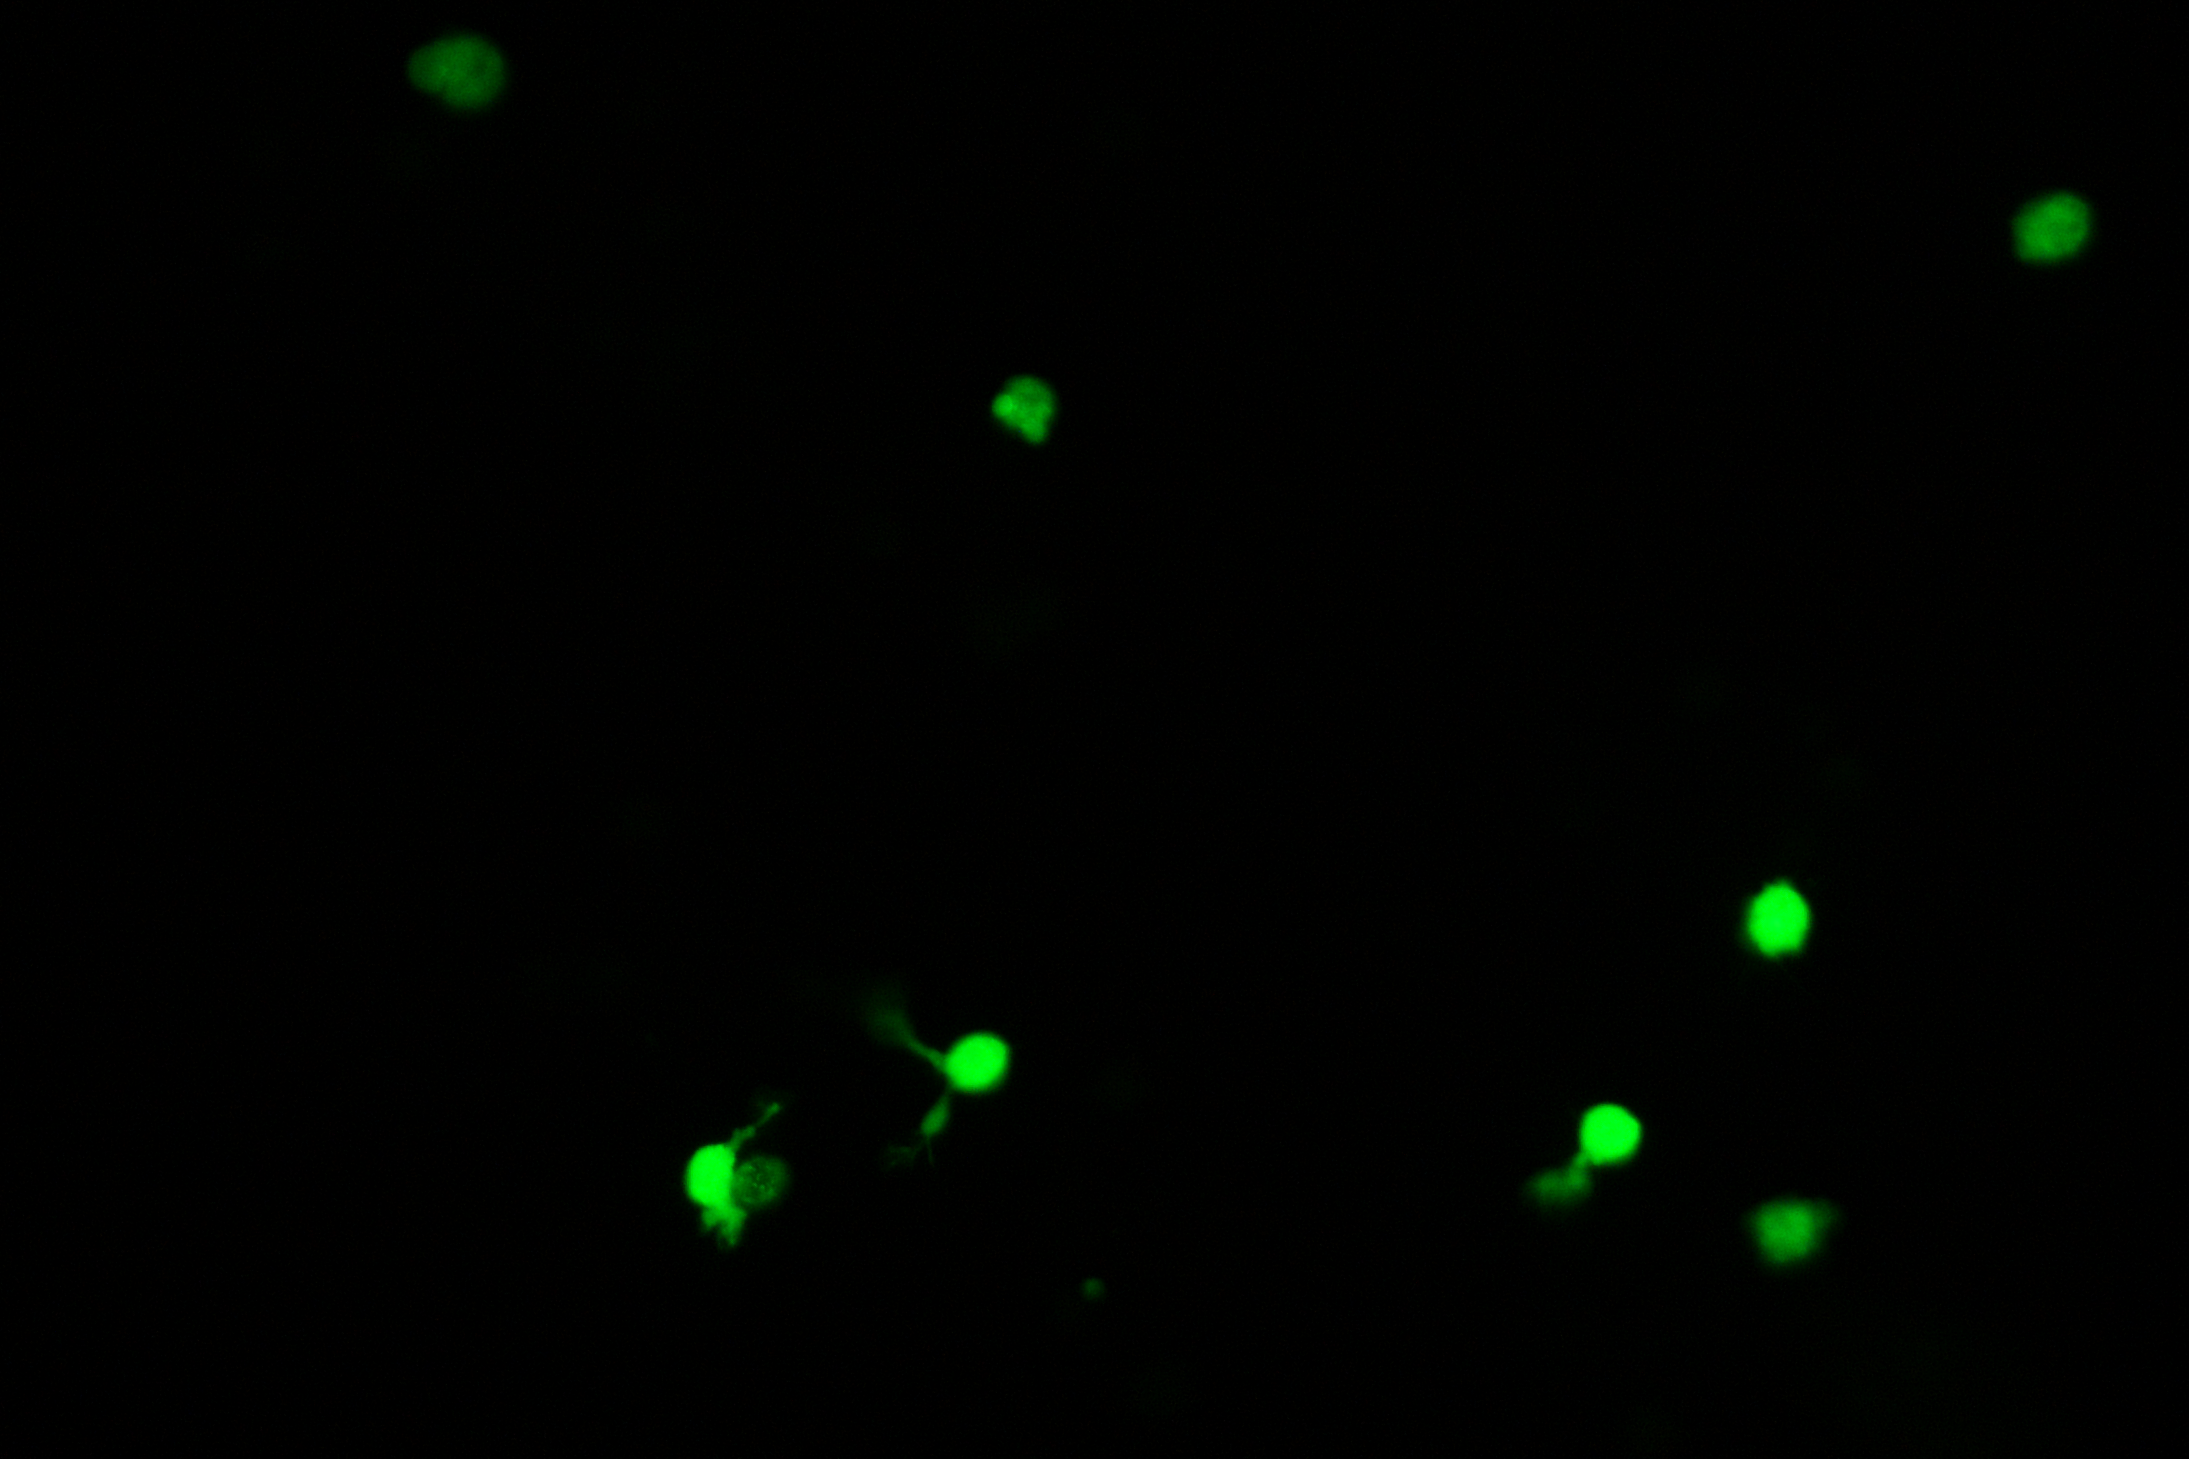
\includegraphics[width=\textwidth]{figures/Method development/Cy5 B2A/M7 7 B2A cropped.png}
        \caption{Calcein fluorescence collected from the same microscopic field with a B-2A filter cube.}
        \label{subfig:b}
    \end{subfigure}
    \newline
    \begin{subfigure}[b]{.45\textwidth}
        \centering
        \includegraphics[width=\textwidth]{figures/Method development/Cy5 B2A/M7 7 DIC cropped.png}
        \caption{Microscopic field imaged by DIC microscopy to verify cellular identities of fluorescent signals.}
        \label{subfig:c}
    \end{subfigure}
    \hfill
    \begin{subfigure}[b]{.45\textwidth}
        \centering
        \includegraphics[width=\textwidth]{figures/Method development/Cy5 B2A/M7 7 Merged cropped.png}
        \caption{Merged RGB image from the red and green color planes of image \emph{a} and \emph{b}, respectively.}
        \label{subfig:d}
    \end{subfigure}
    \caption{An illustration of the image analysis used to score necrotic and viable haemocytes by epifluorescence and DIC microscopy at 20x magnification.}
    \label{fig:Epifluorescent_scoring}
\end{figure}

Following flow cytometric acquisition, the 10 samples were transferred onto glass slides, coverslipped and put on the stage of a Nikon 90i upright microscope equipped with a DS-Fi1c microscope camera (Nikon, Tokyo, JP). Ten microscopic fields were imaged per slide at 20x magnification, and each field was imaged in three subsequent steps (see Figure \ref{fig:Epifluorescent_scoring}): (1) Epifluorescence microscopy with a LED-Cy5-A filter cube, 6 s exposure and 4.8 gain (2) epifluorescent microscopy with a B-2A filter cube, 400 ms exposure and 2.0 gain, followed by (3) DIC microscopy. The red and green color planes of the two epifluorescence images were merged into an RGB image in NIS Elements D software (v.3.22.15), and the percentages of necrotic, viable and doubly stained haemocytes were scored using the merged image (see Figure \ref{fig:Epifluorescent_scoring}d). The DIC images were used to confirm the identity of the fluorescent signals, such that only cellular signals were included in the counts.

The validity of the flow cytometric assay was evaluated by linearity of response after \cite{Ericson2021}, while the accuracy were determined from the mean percent error relative to the epifluorescence microscopy data. The percentage of necrotic haemocytes (Calcein$^{-}$ ToPro3$^{+}$) from flow cytometric and epifluorescence microscopy analyses were analyzed by simple linear regression. The percentage of necrotic haemocytes (\%) were calculated according to (\ref{eq:necrotic hemocytes_2}), such that double positive haemocytes were counted as viable. The imaging process took up to one 1 hour per slide, so any double positive haemocytes had most likely become necrotic during the course of microscopy. It should be noted that samples were prepared and scored one at a time to minimize the occurrence of \emph{in vitro} necrosis.

\begin{equation}
    \label{eq:necrotic hemocytes_2}
    \text{Necrotic haemocytes (\%)} = \dfrac{n_{Calcein^{-}ToPro3^{+}}}{n_{total} - n_{Calcein^{-}ToPro3^{-}}} \times 100
\end{equation}


\subsection{Scoring of apoptotic haemocytes by flow cytometry}
The Annexin V/PI assay is considered the the gold standard of \emph{in vitro} apoptosis detection, but requires free Ca$^{2+}$. This is what to begin this introduction with.
\subsubsection{Determination of optimal Apo-15 staining concentration}
Describe in detail how this probe was dissolved in DMSO and diluted to obtain aliqouts of 8 \micro M. Find the tested concentration in the notebook.
\subsubsection{Gating strategy}





\begin{table}[H]
	\centering
	\caption{The \acrshort{fcm} acquisition and fluidics settings specified with the BD Accuri C6 Plus acquisition software during the flow cytometric experiments reported in this work.}
	\label{tb:FCM_settings}
	\resizebox{\linewidth}{!}{
	\begin{tabular}{lllll}
	\textbf{Experiment nr.} & \textbf{Event-triggering threshold} & \textbf{Acquisition stop-condition} & \textbf{Flow rate (\micro L/min)} & \textbf{Core size (\micro m)} \\
		\midrule
    Aggregation & 80.000 FSC-H & acquired volume, 20 \micro L & 30 & 10 \\
    Calcein AM and TO-PRO$^{TM}$-3 Iodide & 80.000 FSC-H & 10.000 haemocyte events & 36 & 16 \\
    Apo-15 and TO-PRO$^{TM}$-3 Iodide & 80.000 FSC-H & 10.000 haemocyte events & 36 & 16 \\
		\bottomrule
	\end{tabular}
	}
\end{table}

Concider including a simple table with Fluorescent marker (ToPro3, Calcein, Apo15), "measured parameter", exitation laser and Fluorescent filter. Maybe combine with info from the table above?
\chapter{Results}
\label{chap:results_method_development}

\section{Haemocyte medium}
The following section presents results from three experiments that were conducted to explore the suitability of three anticoagulant haemocyte media for flow cytometric applications. They are evaluated with regard to their ability to inhibit haemocyte aggregation - without affecting the viability of haemocytes.

\subsection{Inhibition of haemocyte aggregation}
The proportions of aggregated haemocytes in \acrshort{mpss}, \acrshort{acb} and \acrshort{mas} are plotted against time post-withdrawal in Figure \ref{fig:aggregation}, together with their predicted mean proportions, or more accurately: the predicted proportion of aggregated haemocytes in mussels with random effects $\gamma_{0i}$ and $\gamma_{1i}$ = 0. Predictions were made from the estimated fixed effects in order to address the marginal effect of "Buffer" on the population-averaged proportions. The estimated regression coefficients of the generalized linear mixed effect model is presented in Table \ref{tb:regression_table}, while the fixed effect sub-models are shown in (\ref{eq:mixed_submodels}).

\begin{equation}
    \label{eq:mixed_submodels}
    y_{ij} = \begin{cases}
        \dfrac{1}{1 + e^{-(-1.7192 + 0.5516 \times log(t_{ij}))}}  & i \: \text{in MPSS group}, \\
        \dfrac{1}{1 + e^{-(-6.9842 + 1.8400 \times log(t_{ij}))}}  & i \: \text{in ACB group}, \\
        \dfrac{1}{1 + e^{-(-7.7198 + 2.0138 \times log(t_{ij}))}}  & i \: \text{in MAS group} \\
    \end{cases}
\end{equation}

Figure \ref{fig:aggregation}D unambiguously demonstrates that both \acrshort{acb} and \acrshort{mas} exerted an immediate decelerating effect on the rate of haemocyte aggregation. This inhibitory effect is evident from the estimated differences in slopes and intercepts from the MPSS sub-model, which were significantly different from zero (see Table \ref{tb:regression_table}). Since the effect sizes are a bit challenging to interpret from the isolated coefficients, the linear predictors of the three sub-models are evaluated on link scale in Figure \ref{fig:LogOdds}, i.e. as the log odds of the proportion of aggregated haemocytes ($log P(y_{ij} = 1) / P(y_{ij} = 0)$).

\begin{figure}[!ht]
    \centering
    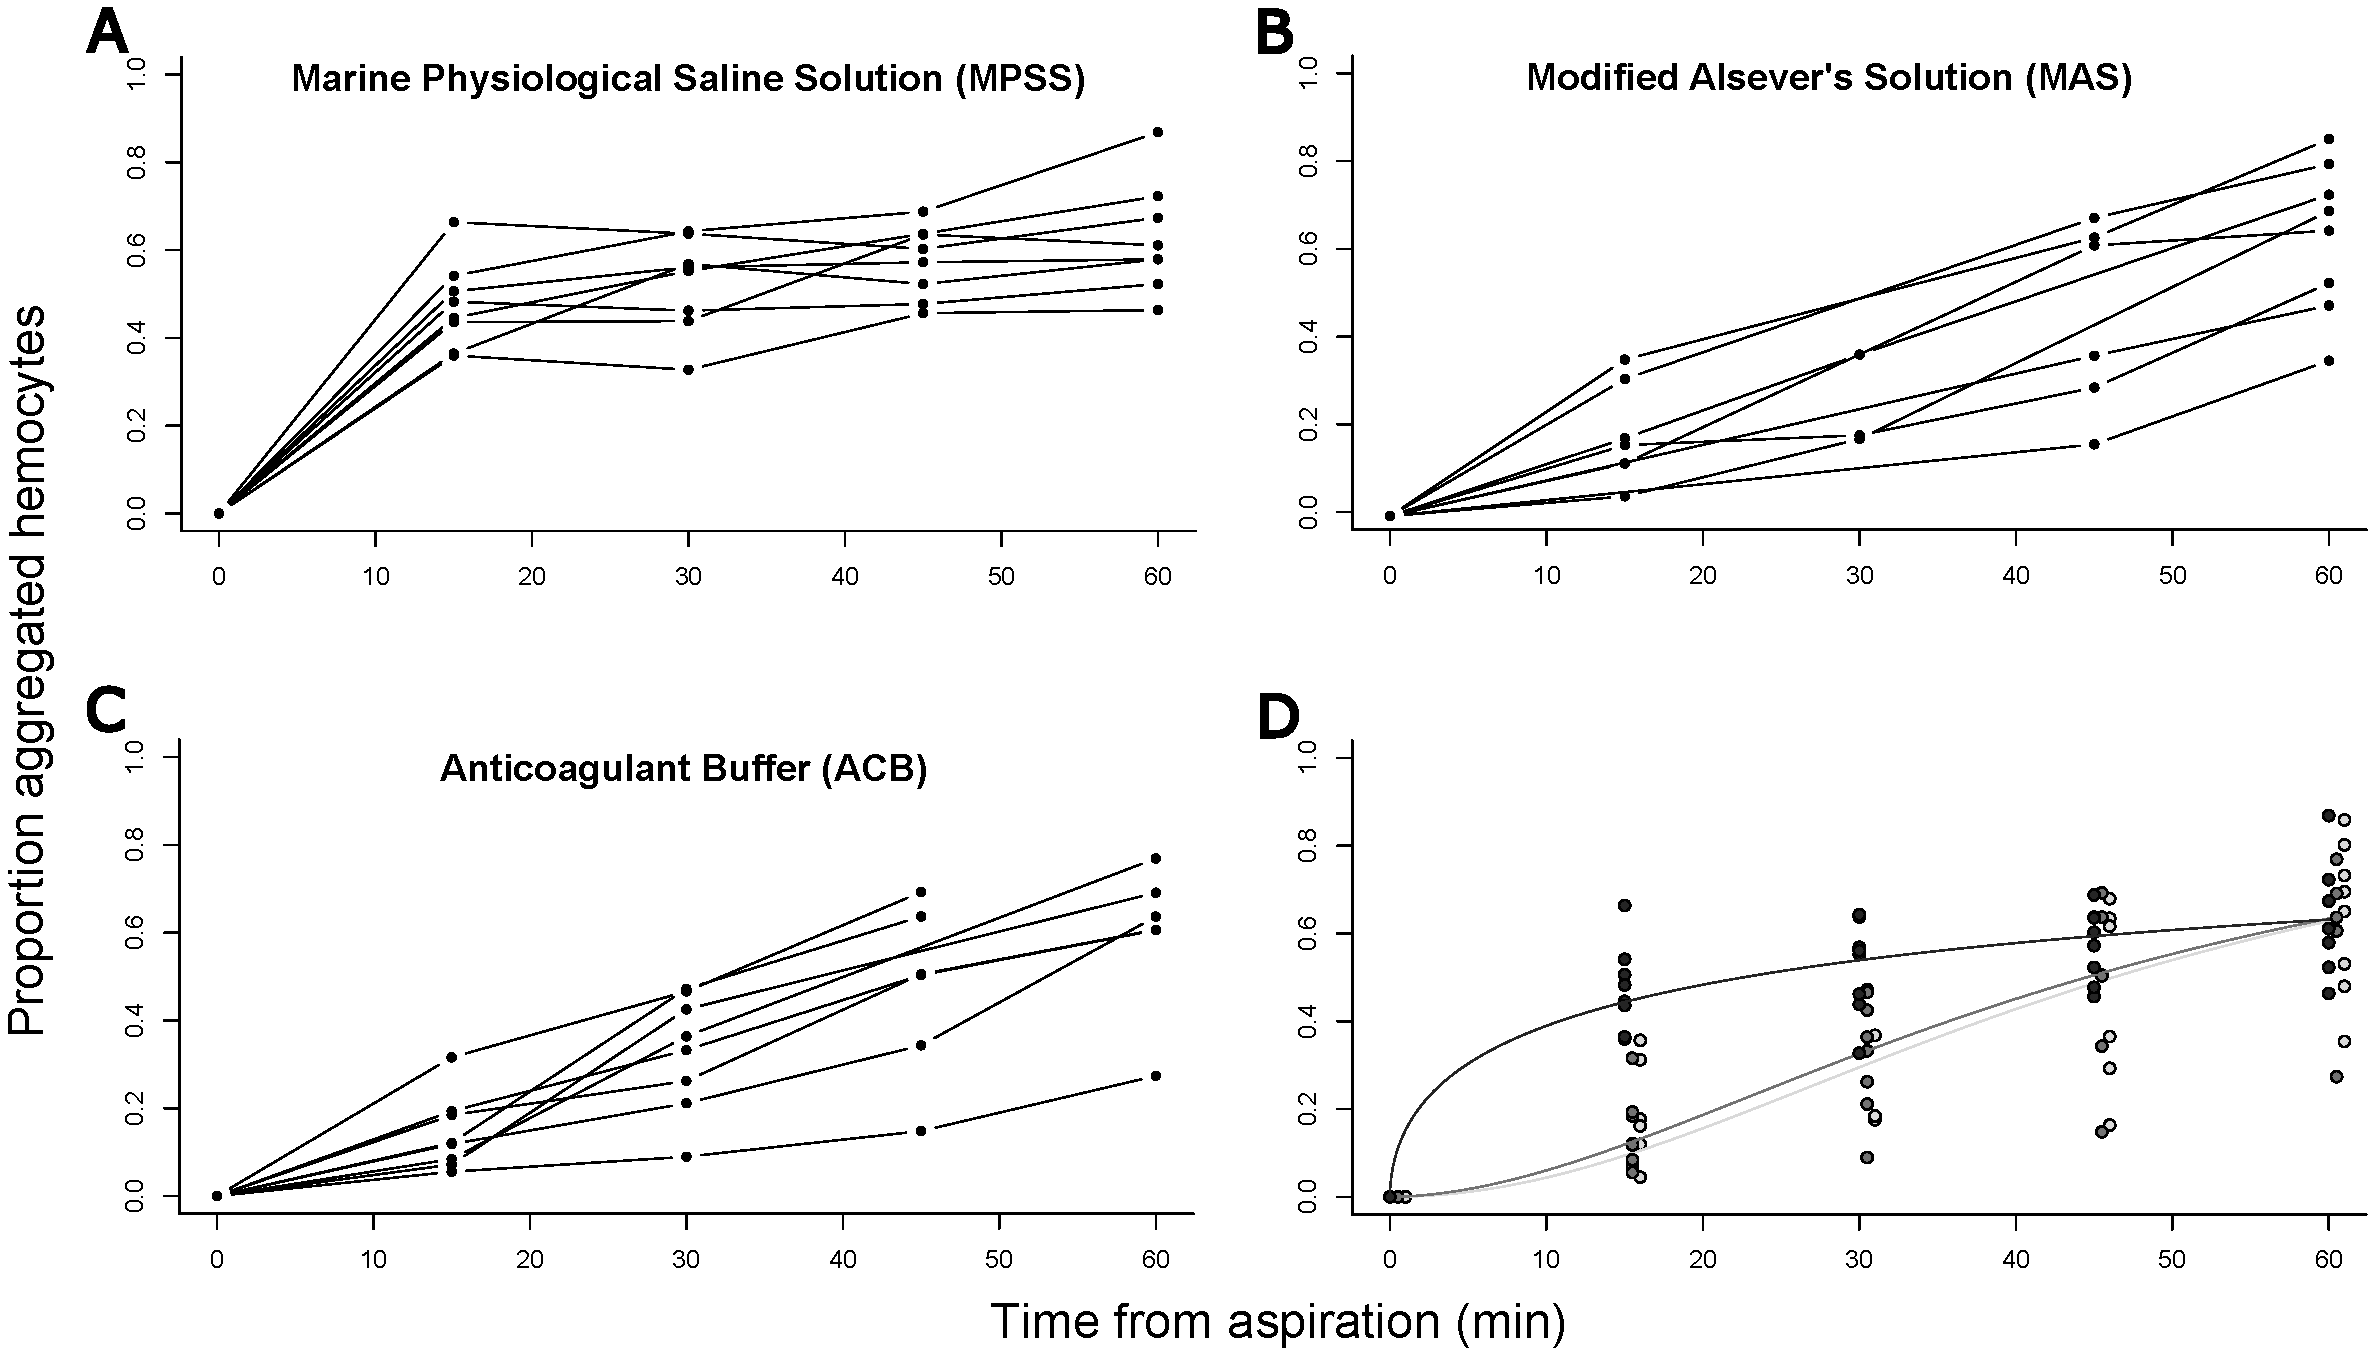
\includegraphics[width=1.0\textwidth]{figures/Method development/Propagg x4 plot.pdf}
    \caption{\textbf{Inhibition of hemocyte aggregation from withdrawing samples into three different anticoagulant buffers.} The proportion of aggregated hemocytes is plotted against time from haemolymph withdrawal after diluting samples in an equal volume of \textbf{A)} Marine Physiological Saline Solution (\acrshort{mpss}, n=8), \textbf{B)} Modified Alsever's Solution (\acrshort{mas}, n=8) or \textbf{C)} Anticoagulant Buffer (\acrshort{acb}, n=8).  \textbf{D)} The same data is combined into one scatter-plot with regression curves representing the mean proportions of aggregated haemocytes in \acrshort{mpss} (\protect\darkgraycircle), \acrshort{mas} (\protect\lysegraacircle) and \acrshort{acb} (\protect\graycircle), as predicted from the fitted mixed logistic regression model. Note that data-points have been jittered on the x-axis to prevent overlap.}
    \label{fig:aggregation}
\end{figure}

\begin{table}[H]
	\centering
	\caption{Parameter estimates of the fitted mixed logistic regression model and their 95\% confidence intervals. Marginal and conditional R$^{2}$-values are presented as parameters of model fit, together with the model's residual deviance.}
	\label{tb:regression_table}
	\begin{tabular}{llllc}
        \toprule
	\textbf{Covariate} & \textbf{Symbol} & \textbf{Estimate$^{b}$} & \textbf{95\% CI$^{a}$} & \textbf{S.E.}\\
		\midrule
  \emph{Intercept}                          & $\alpha_1$ & -1.72*     & [-3.24, -0.202] & 0.740 \\
  \emph{log(t)}                             & $\beta_1$  & 0.552**    & [0.189, 0.915]  & 0.177 \\
  \emph{Buffer$_{ACB}$}                     & $\alpha_2$ & -5.27***   & [-7.41, -3.11]  & 1.05  \\
  \emph{Buffer$_{MAS}$}                     & $\alpha_3$ & -6.00***   & [-8.18, -3.86]  & 1.06  \\
  \emph{log(t)} $\cdot$ \emph{Buffer$_{ACB}$} & $\beta_2$& 1.29***    & [0.775, 1.80]   & 0.251 \\
  \emph{log(t)} $\cdot$ \emph{Buffer$_{MAS}$} & $\beta_3$& 1.46***    & [0.950, 1.98]   & 0.253 \\
  \emph{SD}$(\gamma_{0i})$                  & $\tau_0^2$ & 2.09       & [1.57, 2.91]    & -     \\
  \emph{SD}$(\gamma_{1i})$                  & $\tau_1^2$ & 0.500      & [0.379, 0.694]  & -     \\
  &&& \\
  \multicolumn{5}{l}{Marginal R$^{2}$ = 0.87$^{c}$} \\
  \multicolumn{5}{l}{Conditional R$^{2}$ = 0.98$^{c}$} \\
  \multicolumn{5}{l}{Residual deviance: 13498 on 98 degrees of freedom} \\
		\bottomrule
  \multicolumn{5}{l}{\footnotesize $^{a}$Computed 95\% confidence intervals based on Likelihood Ratio Test of the profile likelihood.} \\
  \multicolumn{5}{l}{\footnotesize $^{b}$ *, **, *** indicates statistical significance on 95\%, 99\% and 99.9\% confidence levels, respectively.} \\
  \multicolumn{5}{l}{\footnotesize Confidence levels were obtained from z-statistics of the asymptotic Wald test.} \\
    \multicolumn{5}{l}{\footnotesize $^{c}$Calculated according to the method proposed by Nakagawa and Schielzeth (2013).} \\
	\end{tabular}
\end{table}

\begin{figure}[!ht]
    \centering
    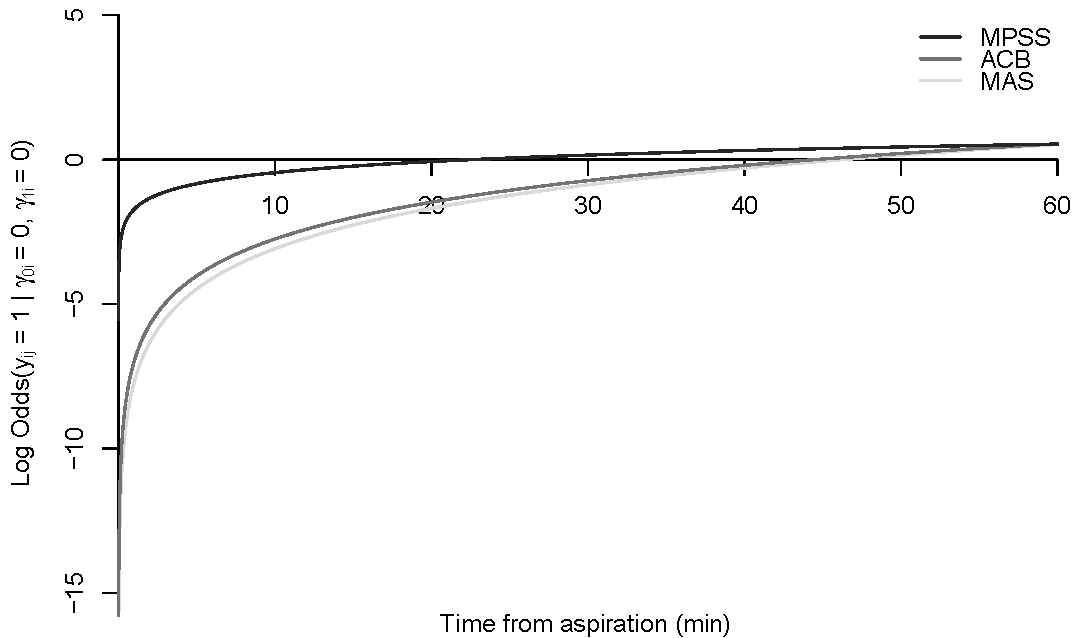
\includegraphics[width=1.0\textwidth]{figures/Method development/Log Odds plot.pdf}
    \caption{The log odds of the proportion of aggregated haemocytes ($log P(y_{ij} = 1) / P(y_{ij} = 0)$) is plotted against time (min) after haemolymph withdrawal, when samples were withdrawn into an equal volume of Marine Physiological Saline Solution (MPSS), Anticoagulant Buffer (ACB) or Modified Alsever's Solution (MAS). The three curves illustrates the logit-scaled predictions of the fitted mixed logistic regression model for the three buffers.}
    \label{fig:LogOdds}
\end{figure}

Given the that the predicted proportion of aggregated haemocytes is 0.50 when the log odds is equal to zero, Figure \ref{fig:LogOdds} shows that 1/2 of the haemocytes withdrawn into \acrshort{mpss} had aggregated within 23 minutes post-withdrawal. This interpretation is valid when the random effects of individual mussels ($\gamma_{0i}$ and $\gamma_{1i}$) are equal to zero. For samples withdrawn into \acrshort{acb} or \acrshort{mas} on the other hand, the haemocytes did not achieve this degree of aggregation until 45 and 46 minutes post-withdrawal, respectively. The three log odds curves depicted in Figure \ref{fig:LogOdds} shows that the inhibitory effects of \acrshort{acb} and \acrshort{mas} were modelled through their significantly lower y-intercepts compared to the \acrshort{mpss} sub-model (Table \ref{tb:regression_table}). These estimates were significant after accounting for within-mussel correlations (Table \ref{tb:regression_table}).

The inhibitory effect was largest during the initial 15-20 minutes, before the degree of aggregation slowly approached that of \acrshort{mpss} around 60 minutes post-withdrawal. In haemolymph samples withdrawn into \acrshort{acb} or \acrshort{mas}, the mean proportions of aggregated haemocytes after 15 minutes were 0.14 95\% CI [0.07, 0.22] and  0.20 95\% CI [0.07, 0.32], respectively. There was no significant difference between the two \acrshort{edta}-containing buffers, but both \acrshort{acb} and \acrshort{mas} had significantly lower proportions at this timepoint compared to samples withdrawn into cold \acrshort{mpss} (0.48 95\% CI [0.39, 0.56]).

\subsection{EDTA cytotoxicity}
 The mean percentages of necrotic hemocytes in \acrshort{mpss}, \acrshort{acb} and \acrshort{mas} after 15 minutes, 2 hours and 20 hours incubation are presented in Figure \ref{fig:BufferViability}, with error bars representing 95\% confidence intervals around group means. Within group differences in means at the three incubation periods are presented Table \ref{tb:Paired_ttests}.

\begin{figure}[H]
    \centering
    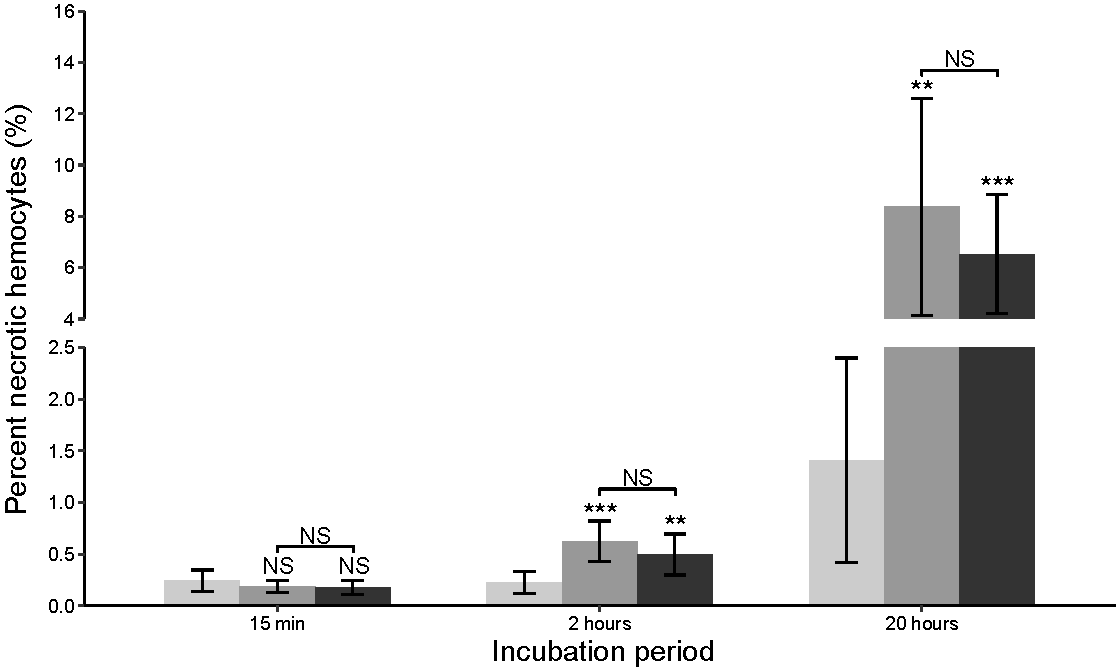
\includegraphics[width=0.75\textwidth]{figures/Method development/EDTA cytotoxicity.pdf}
    \caption{The mean percentages of TO-PRO$^{TM}$-3 Iodide positive hemocytes after 15 minute, 2 hours and 20 hours incubation in Marine Physiological Saline Solution (\, \protect\lysegraabox, \ n=8), Anticoagulant Buffer (\, \protect\customgraybox, \ n=8) and Modified Alsever's Solution (\, \protect\darkgraybox, \ n=8). Error bars represent 95\% confidence intervals around group means, *, **, *** above error bars denotes confidence level of one-tailed two sample t-test comparisons with the \acrshort{mpss} control group, while asterisks above horizontal lines represent \acrshort{acb} vs. \acrshort{mas} comparisons. NS: Not Significant.}
    \label{fig:BufferViability}
\end{figure}

The difference between the negative control group (\acrshort{mpss}) and the two \acrshort{edta}-containing buffers were not significantly different from zero after 15 minute incubation. But as the incubation period was increased to 2 and 20 hours, the percentages of necrotic haemocytes in \acrshort{acb} and \acrshort{mas} increased relative to the negative control group. After 2 hours incubation, there were 0.40\% and 0.27\% more necrotic haemocytes in \acrshort{acb} (t(14) = 4.29, p<.001) and \acrshort{mas} (t(14) = 2.86, p=.006) compared to cold \acrshort{mpss}, respectively. After 20 hours incubation, these differences had increased to 6.96\% (t(14) = 3.78, p=.003) and 5.12\% (t(14) = 4.82, p<.001).

The mean percentage of necrotic haemocytes increased significantly with the incubation period in both MAS and ACB (Table \ref{tb:Paired_ttests}). Since the concentration of EDTA was constant across all timepoints, this increase was dose-dependent as the exposure duration was the only variable factor. There were no significant increase in the percentage of necrotic haemocytes in MPSS from 15 minutes to 2 hours incubation, but a significant increase of 1.184\% was observed after 20 hours (p<.026).

\begin{table}[h!]
\centering
	\caption{Paired two-tailed t-tests were used to assess wether the percentages of necrotic haemocytes increased with incubation time within each group. The difference between means at t = 15 min, 2 hours and 20 hours are presented with 95\% confidence intervals and the belonging p-value.}
	\label{tb:Paired_ttests}
        \resizebox{\linewidth}{!}{
	\begin{tabular}{c|ccccc}
		\toprule
		\multirow{2}{*}{Buffer} & \multicolumn{2}{c}{\textbf{Paired t-test comparison}} & \multirow{2}{*}{Difference (\%)} & \multirow{2}{*}{95\% CI} & \multirow{2}{*}{Pr(T > $\mid$ t $\mid)$} \\
		& Incubation \emph{t} & Incubation \emph{t - 1} & & & \\
		\midrule
     \multirow{2}{*}{MPSS} &  2 hours  &  15 min  & -0.018 & [-0.023, -0.015] & .78 \\
     &  20 hours &  2 hours & 1.184  & [1.157, 1.211]   & .026 \\
    \multirow{2}{*}{ACB} &   2 hours  &  15 min  & 0.438  & [0.433, 0.444]   & .00187 \\
       &   20 hours &  2 hours & 7.742  & [7.627, 7.857]   & .00324 \\
    \multirow{2}{*}{MAS} &   2 hours  &  15 min  & 0.319  & [0.313, 0.324]   & .00690 \\
        &   20 hours &  2 hours & 6.037  & [5.970, 6.105]   & <.001 \\
		\bottomrule
	\end{tabular}
 }
\end{table}


\subsection{Cytotoxicity of acidic haemocyte medium pH}
The mean percentage of early and late apoptotic haemocytes after 15 minutes incubation in non-adjusted Modified Alsever's Solution (\acrshort{namas}, pH = 6.1) and Anticoagulant Buffer (ACB, pH = 7.6) is presented as bargraphs in Figure \ref{fig:pH_Apo}, with error bars representing 95\% confidence intervals around group means. 

\begin{figure}[H]
    \centering
    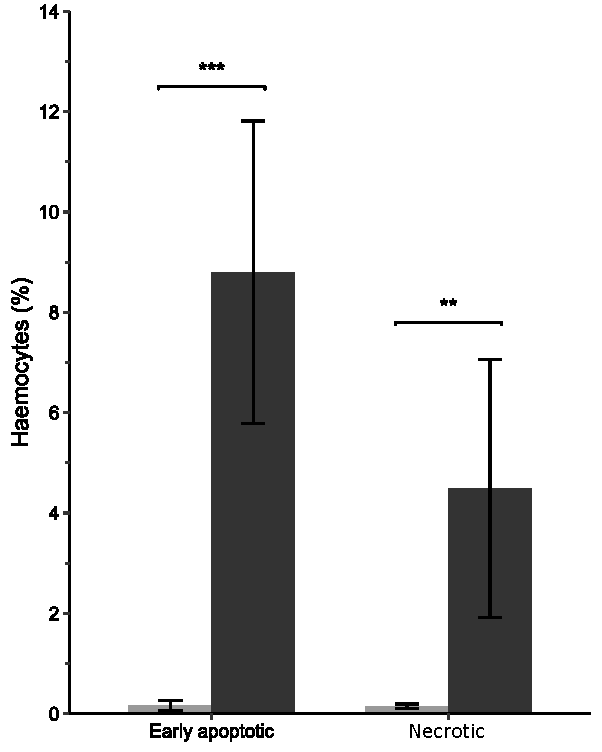
\includegraphics[width=0.5\textwidth]{figures/Method development/Apo15 pH 2.pdf}
    \caption{The mean percentage of early apoptotic (Apo15$^{+}$/ToPro3$^{-}$) and late apoptotic haemocytes (Apo15$^{+}$/ToPro3$^{+}$) after 15 minutes incubation in Anticoagulant Buffer (\, \protect\customgraybox, \ n=18) and non-adjusted Modified Alsever's Solution (\, \protect\darkgraybox, \ n=18). Error bars represent 95\% confidence intervals around group means. Asterisks *, **, *** denotes confidence level of one-tailed two sample t-test comparisons.}
    \label{fig:pH_Apo}
\end{figure}

Haemocytes that were incubated in the acidic MAS buffer showed a significant induction of apoptosis relative to samples kept in ACB. The mean percentage of early apoptotic haemocytes in naMAS were 53 times higher than in ACB (t(17) = 6.04, p<.001), while that of necrotic haemocytes were 31 times higher (t(17) = 3.57, p=.00117). The percentages of necrotic and early apoptotic haemocytes in ACB were consistently low, with mean percentages of 0.144$\pm{0.09}$\% and 0.165$\pm{0.2}$\%, respectively.

\section{Development of a flow cytometric differential count}
This section presents the results of several experiments that were conducted in order to develop and validate a flow cytometric differential count of the cell types present in the haemolymph of \emph{M. edulis}. Section \ref{subsection:CytCar} presents a cytological characterization of the haemocytes according to i.a., cell size, granularity and staining affinities in accordance with the current scientific practice in invertebrate immunology. The flow cytometric characterization in section \ref{subsection:Results_FlowChar} presents the subpopulations of haemocytes that were separated according to FSC (relative size) and side scatter (internal complexity), and put these results in context of the cytologically defined cell types. The next section (\ref{subsection:evidence}) presents results from two experiments that were aimed to uncover the relationship between the cytologically defined cell types and the subpopulations discernible by light scatter measurements. Lastly, the gating strategy for the differential haemocyte count is presented with proof of concept.

\subsection{Cytologic characterization of \emph{M. edulis} hemocyte subpopulations}
\label{subsection:Results_cytchar}
The hemolymph of \emph{Mytilus edulis} comprised a mixed population of cells differing in size, granularity, morphometrics and Wright's-Giemsa staining profiles. If the haemocytes were allowed to spread prior to fixation and staining, the diversity further expanded as cells took on a variety of shapes and/or developed cytoplasmic extensions. From these morphological criteria, a total of three distinct cell types could be identified by light microscopy.

Based on the basophilic or eosinophilic nature of their granules and other cytoplasmic contents, cytologic staining with 3 \% Wright's-Giemsa or the Hemacolor\textsuperscript{\textregistered} kit gave rise to two distinct staining profiles: basophilic and eosinophilic haemocytes. The cytoplasm of eosinophilic hemocytes (Figure \ref{fig:celltypes}, K-O) were densely packed with pink to dark purple granules of varying size and abundance. Hence, they are referred to as eosinophilic granulocytes herein. Their individual granules were usually not distinguishable in a non-spread state, but instead gave their cytoplasm an irregular pink color (Figure \ref{fig:celltypes}, K and O). These haemocytes had cell diameters in the range of 6-16 \micro m, with a mean of 9.06$\pm1.25$ \micro m. Two strikingly homogeneous features of this cell type was a small acentrically located nucleus, and a regular spherical outline in a non-spread state. With abundant pink cytoplasm making up the majority of the cells' surface area - even in the smallest specimens - the eosinophilic granulocytes could also be characterized by a low nuclear-cytoplasmic ratio (N:C ratio). If not fixed and stained before smearing - or within minutes of applying haemolymph to a glass slide - eosinophilic granulocytes were almost exclusively observed as spread cells. 

\begin{figure}[H]
    \centering
    \includegraphics[width=1.0\textwidth]{figures/Anatomy/cell types brightfield updated 2.pdf}
    \caption{100$\times$ brightfield micrographs of the three haemocyte types found in the haemolymph of \emph{Mytilus edulis}, fixed and stained on glass slides with the Hemacolor\textsuperscript{\textregistered} kit before the hemocytes had time to spread notably. \textbf{(A-E)} Blast-like hyaline basophils. \textbf{(F-J)} Basophilic granulocytes. \textbf{(K-O)} Eosinophilic granulocytes. Samples were withdrawn into \acrshort{mpss} (1:1), scale bars = 10 \micro m.}
    \label{fig:celltypes}
\end{figure}

Compared to the eosinophilic granulocytes, the basophilic hemocytes encompassed a more heterogeneous population. Common to all of them were a larger nucleus that occupied more of the cells' total surface area (higher N:C ratio). The shape of which varied from spherical to oval, or had a distinct bean-shaped or irregular outline. But judged from the morphological criteria of cell size, granularity and N:C ratio, there were essentially two distinct subpopulations of basophilic haemocytes: one population of small hyaline blast-like haemocytes (5.63 $\pm{0.72}$ \micro m) displaying only a marginal rim of dove blue cytoplasm and no apparent cytoplasmic granules (Figure \ref{fig:celltypes}, A-E), and one population of larger haemocytes (8.07 $\pm{1.25}$ \micro m), displaying abundant basophilic cytoplasm with varying degrees of cytoplasmic granulation and vacuolation (Figure \ref{fig:celltypes}, F-J). The basophillic granules appeared much smaller than those of the eosinophilic granulocytes, and were usually not very conspicuous unless haemocytes were subjected to osmotic swelling prior to fixation and staining. Under differential interference contrast (DIC) illumination however, their granules created highly irregular surface topographies in spread cells that could be observed without such treatment. On the basis of these morphological differences, the basophilic haemocytes were subdivided into blast-like haemocytes and basophilic granulocytes herein. 

\begin{figure}[H]
    \centering
    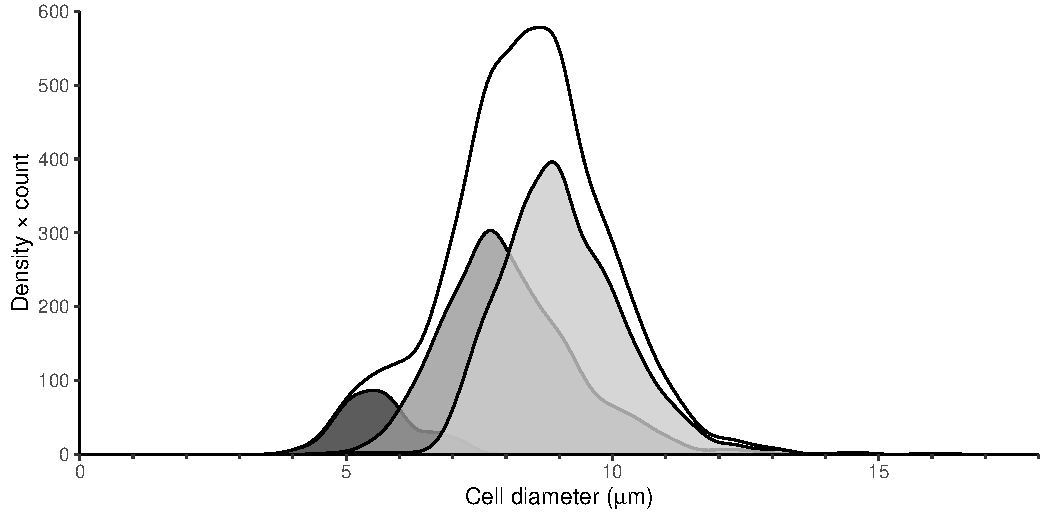
\includegraphics[width=1.0\textwidth]{figures/Anatomy/diameters scaled density plot.pdf}
    \caption{Size distribution of \protect\dimgraybox \ small blast-like basophils (n=154), \protect\lightgraybox \ basophilic granulocytes (n=821), \protect\lysegraabox \ eosinophilic granulocytes (n=1030) and \protect\whitebox \ the total haemocyte population of \emph{Mytilus edulis} (n=2005). The diameters of 100 formaldehyde-fixed haemocytes were measured in each of 20 individual mussels, and the density was scaled to the number of observations of each cell type.}
    \label{fig:Diameters}
\end{figure}

The size distributions of the three haemocyte types are shown as three kernel-smoothened density plots in Figure \ref{fig:Diameters}, together with that of the total haemocyte population. The densities have been scaled to the number of observations of each cell type, such that their relative proportions can be visualized. In the 20 adult mussels examined here, the small blast-like basophils were the least abundant cell type, making up 7.9 $\pm{5.6}$\% of the total haemocyte population. In 14 out of 20 mussels, the blast-like basophils were followed by the basophilic granulocytes, with a mean relative proportion of 40.7 $\pm{12.9}$\%. In spite of constituting similar proportions as the basophilic granulocytes in several mussels, the eosinophilic granulocytes were the most abundant cell type in the haemolymph of \emph{M. edulis}, constituting 51.5 $\pm{15.3}$\% of the total haemocyte population, on average. The relative proportions of basophilic and eosinophilic granulocytes did however vary to a large extent between individual mussels, as reflected by their standard deviations.

\subsection{Flow cytometric characterization of haemocyte subpopulations by light-scatter}
\label{subsection:Results_FlowChar}
A maximum of three distinct subpopulations could be separated according to Forwards scatter (FCS) vs. Side scatter (\acrshort{ssc}) in suspensions of living haemocytes. These comprised one subpopulation of events with low \acrshort{fsc}- and \acrshort{ssc}-values, one with high \acrshort{fsc}- and intermediate \acrshort{ssc}-values and one with high \acrshort{fsc} and \acrshort{ssc}. The aforementioned subpopulations correspond to clusters 1, 2 and 3 in Figure \ref{fig:fsc_vs_ssc}, where the haemocytes of three representative mussels have been displayed with \acrshort{ssc} on logarithmic and linear scales.

The adjunct histograms in Figure \ref{fig:fsc_vs_ssc}A and B clearly illustrates that the three clusters of events are separated according to log \acrshort{ssc}, while there is substantial overlap between cluster 2 and 3 with regard to \acrshort{fsc}. The latter feature was consistent across all mussels, while the degree of separation according to log \acrshort{ssc} was subject to individual variation. In this regard, the haemolymph sample presented in \ref{fig:fsc_vs_ssc}B represents a typical mussel, i.e., with cluster 2 and 3 incompletely separated according to log \acrshort{ssc}. The samples presented in \ref{fig:fsc_vs_ssc}A and C represents the extreme ends of this variation, with complete separation and complete overlap, respectively.

Since \acrshort{fsc} and \acrshort{ssc} can be interpreted as relative measures of cell size and internal complexity, these results suggests that the haemolymph of \emph{M. edulis} are comprised of three cell types that are distinguishable according to size and internal complexity. The events populating cluster 1 exhibited low \acrshort{fsc}- and \acrshort{ssc}-values relative to cluster 2 and 3, indicating that it is populated by haemocytes that are both smaller and less complex than the rest of the haemocytes. If \acrshort{ssc} is interpreted more specifically in terms of haemocyte characteristics, the events populating cluster 2 and 3 most likely correspond to large semi-granular haemocytes and large granulocytes, respectively.

\begin{figure}[ht!]
    \centering
    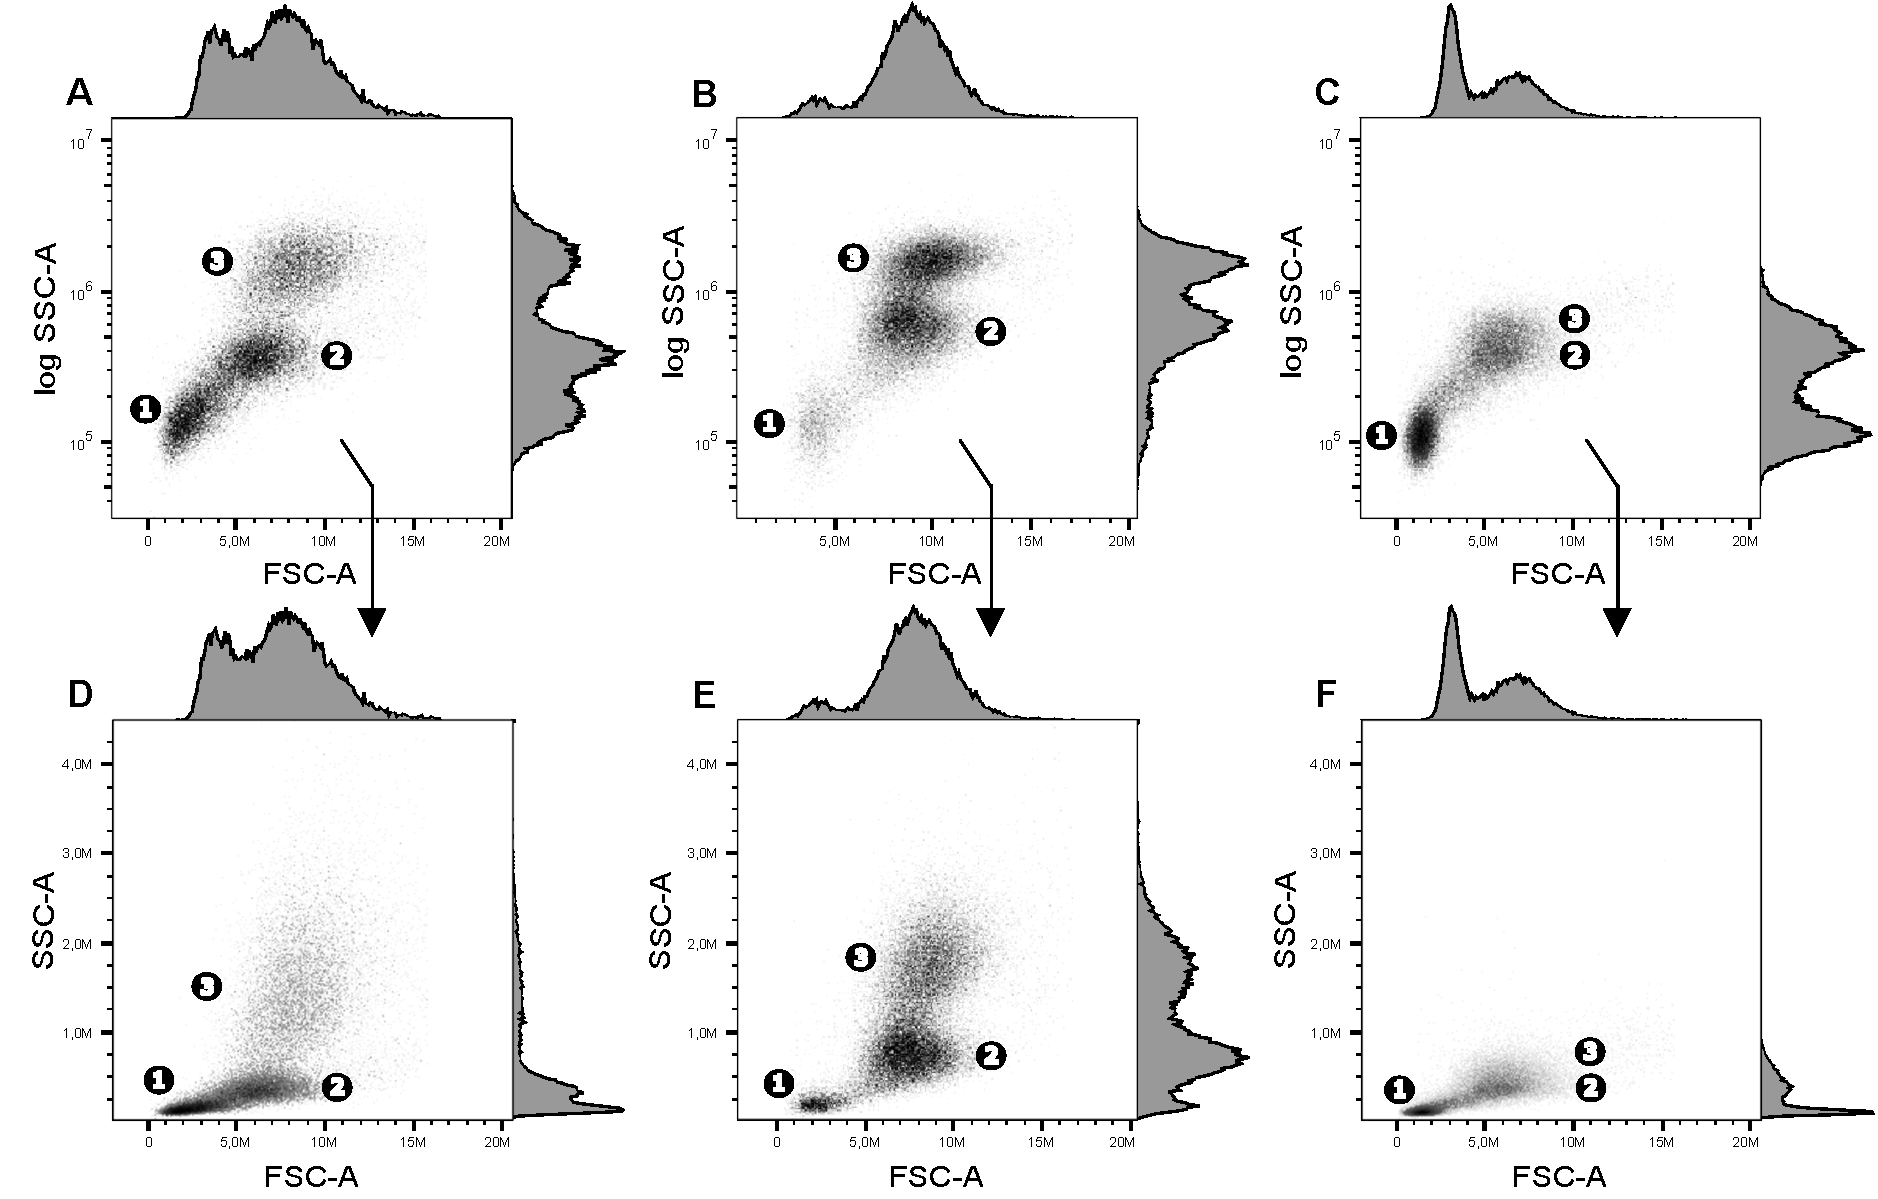
\includegraphics[width=1.0\textwidth]{figures/Gating strategy/The three musceteers.pdf}
    \caption{\textbf{Haemocyte subpopulations distinguishable according to \acrshort{fsc} and \acrshort{ssc} measurements with the BD Accuri C6 Plus Benchtop Flow Cytometer.} The light-scatter profiles of three representative adult mussels are displayed with \acrshort{ssc} on logarithmic \textbf{(A-C)} and linear \textbf{(D-F)} scales to illustrate the observed variation in the degree of separation between cluster 2 and 3. Adjunct histograms were included to illustrate the degree of separation contributed from each parameter individually.}
    \label{fig:fsc_vs_ssc}
\end{figure}

\subsection{Relating cytologically defined cell types to light-scatter profiles}
\label{subsection:evidence}
\subsubsection{Flow cytometric characterization of haemocytes pre-separated by isopycnic centrifugation }
Formaldehyde-fixed haemocytes separated into three distinct cell-bands on the 15/33\%, 38/43\% and 43/90\% gradient interfaces of the discontinuous Percoll gradients. As shown in Figure \ref{fig:Percoll-tubes}, the two upmost bands exhibited a similar blue coloration, while the band located on the 43/90\% interface had a darker purple color. The latter consisted of 96.9$\pm{0.9}$\% eosinophilic granulocytes, with a few basophillic granulocytes scattered among them. From the cell bands located at the 15/33\% interface, a populations of 96.3$\pm{0.2}$\% basophillic haemocytes were isolated. The majority of these cells were basophilic granulocytes (87.5$\pm{1.2}$\%), with a smaller fraction of blast-like basophils (8.8$\pm{1.5}$\%). The middle bands did not yield any of the cell types in high purity, but were predominantly populated by basophilic granulocytes (72.7$\pm{1.5}$\%) with numerous small dark granules.

\begin{figure}[H]
    \centering
    \includegraphics[width=.75\textwidth]{figures/Method development/Percoll tubes.pdf}
    \caption{\textbf{Formaldehyde-fixed haemocytes pre-stained with Giemsa were separated by isopycnic centrifugation on discontinuous Percoll gradients.} The haemocytes settled into three distinct cell bands on the 15/33\%, 38/43\% and 43/90\% gradient interfaces.}
    \label{fig:Percoll-tubes}
\end{figure}

The light scatter profiles of the three isolated cell fractions are depicted in Figure \ref{fig:Percoll-dotplots}, together with that of the unseparated haemocytes. As shown in Figure \ref{fig:Percoll-dotplots}A, the pooled haemocyte were not readily distinguishable as three separate subpopulations prior to centrifugation. Since the relative size and complexity of the three cell types vary slightly between individual mussel, this is a common phenomenon when haemolymph from two or more mussels are pooled together. However, a more distinct clustering was seen among the haemocytes isolated from the middle cell-band (see Figure \ref{fig:Percoll-dotplots}C), where the relative proportions of eosinophilic granulocytes (18.4\%) and blast-like basophils (7.8\%) were lower.

\begin{figure}[H]
    \centering
    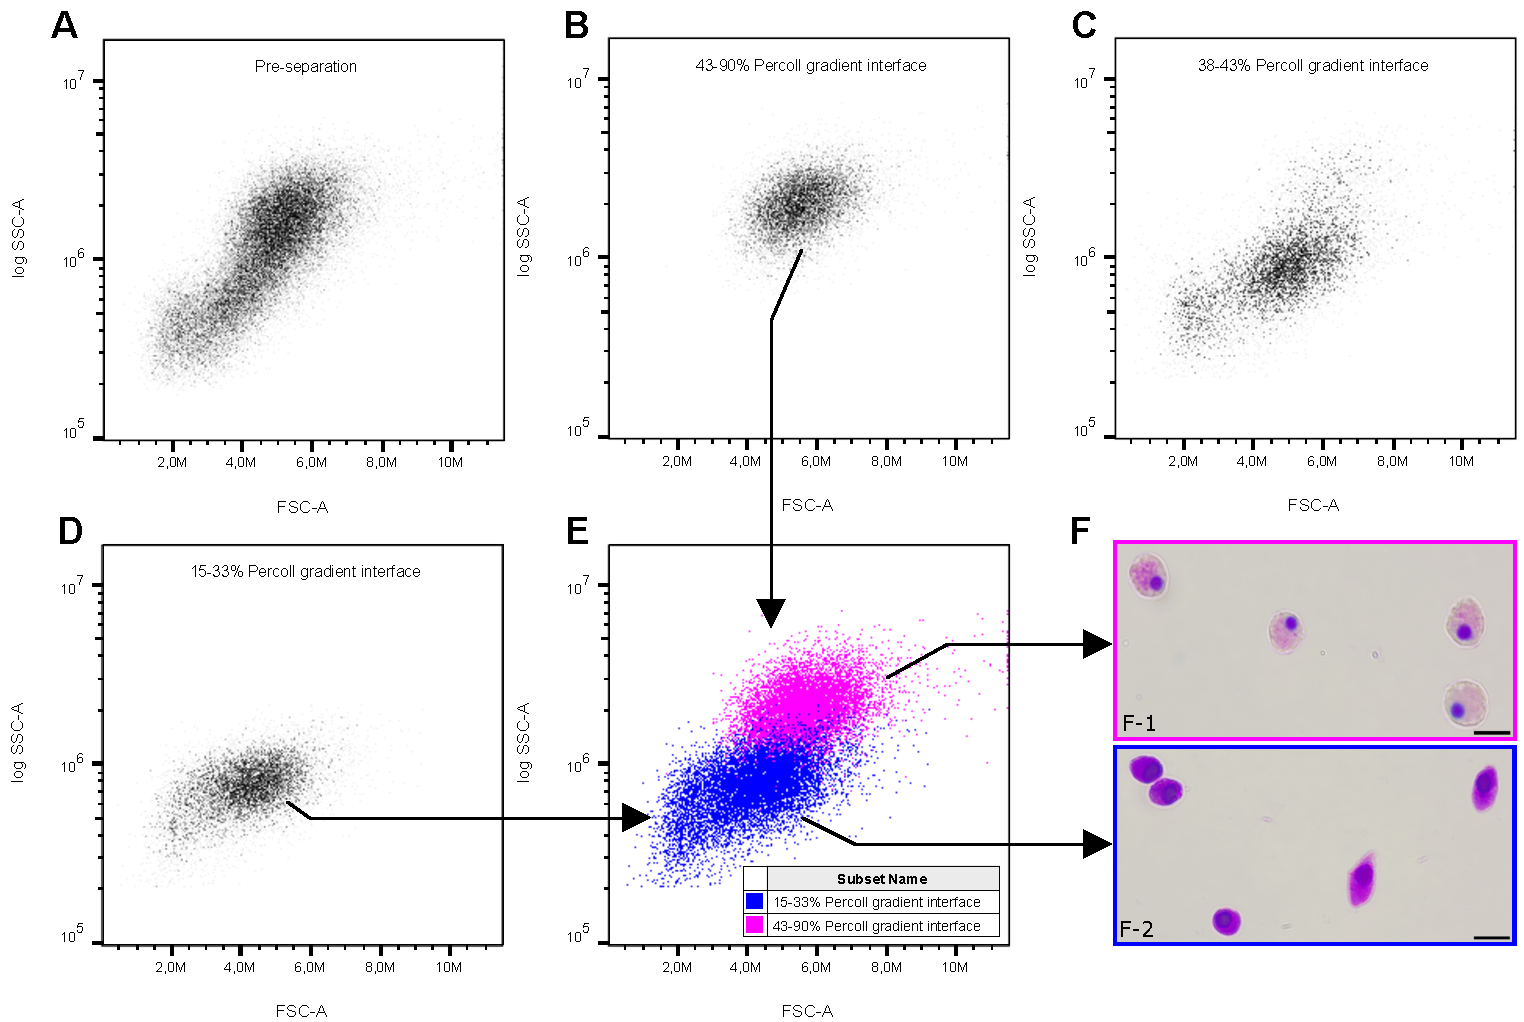
\includegraphics[width=1.0\textwidth]{figures/Method development/PERCOLL SEP II.pdf}
    \caption{\textbf{Flow cytometric analysis of the isolated cells types of \emph{M. edulis} haemolymph after separation by isopycnic centrifugation.} Two pools of formaldehyde-fixed haemocytes were separated by density-dependent centrifugation after the method of Friebel and Renwrantz (1994), and the isolated fractions were analyzed by flow cytometry and light microscopy. FSC vs. log SSC density plots depicts one of the pools prior to centrifugation \textbf{(A)} and after separating into three distinct cell-bands on the gradient interfaces \textbf{(B-D)}. The enriched fractions (> 96\%) of eosinophilic granulocytes \textbf{(B)} and basophilic haemocytes \textbf{(D)} are overlayed in \textbf{(E)}, with micrographs of the respective layers presented in \textbf{(F)}. F-1: eosinophilic granulocytes; F-2: basophilic granulocytes; scale bars = 10 \micro m. }
    \label{fig:Percoll-dotplots}
\end{figure}

The eosinophilic granulocytes formed from the bottom layer a dense cluster of events exhibiting high FSC- and SSC-values (Figure \ref{fig:Percoll-dotplots}B). This is consistent with the expected light scatter profile of this cell type, since they represent highly granulated cells with large cell diameters. The two basophilic cell types from the upper cell band were unambiguously separated from the eosinophilic granulocytes according to SSC, where only a small number of cells exceeded values > 1$\times 10^{6}$ (Figure \ref{fig:Percoll-dotplots}D). This relationship is clearly demonstrated by the overlayed dotplot in Figure \ref{fig:Percoll-dotplots}E, where the eosinophilic granulocytes are shown in pink.

\subsubsection{Identification of eosinophilic granulocytes by eosin fluorescence}
Formaldehyde-fixed haemocytes stained with 0.5\% eosin were separated into distinct eosin$^{bright}$ and eosin$^{dim}$ populations by flow cytometric measurements of eosin fluorescence (Figure \ref{fig:eosin_exp2}B and C). The degree of separation varied to a large extent between individual mussels, but the \acrshort{mfi} of eosin$^{bright}$ events were 11$\pm{9}$ times higher than that of eosin$^{dim}$ events, on average. The difference in fluorescent intensity between eosinophilic and basophilic granulocytes is illustrated in Figure \ref{fig:Eosin_fluorescence_B2A}, where Giemsa-stained haemocytes have been imaged by epifluorescence microscopy with a B-2A filtercube (Em: $\geq$ 515 nm; exposure: 250 msec; gain: 3.4).

\begin{figure}[H]
    \centering
    \begin{subfigure}[b]{.45\textwidth}
        \centering
        \includegraphics[width=\textwidth]{figures/Method development/B2A eosin fluorescence/Epi eosin fluorescence.pdf}
        \caption{Hemocytes imaged under brightfield illumination.}
        \label{ffig:a}
    \end{subfigure}
    \hfill
    \begin{subfigure}[b]{.45\textwidth}
        \centering
        \includegraphics[width=\textwidth]{figures/Method development/B2A eosin fluorescence/Brightfield eosin fluorescence.pdf}
        \caption{Haemocytes imaged by epifluorescence microscopy with a B-2A filtercube.}
        \label{ffig:b}
    \end{subfigure}
    \caption{\textbf{Eosinophilic granulocytes are distinguished from the two basophilic cell types according to eosin fluorescence ($\geq$ 515 nm).} Formaldehyde-fixed haemocytes stained in 0.5\% eosin and 3\% Giemsa were imaged at $\times$60 magnification under \textbf{a)} brightfield illumination and \textbf{b)} by epifluorescence microscopy with a B-2A filter cube. The slide was mounted with Eukitt\textsuperscript{\textregistered} and coverslipped prior to microscopy. Eo: eosinophilic granulocyte; B: basophilic haemocyte; scale bars = 10 \micro m. }
    \label{fig:Eosin_fluorescence_B2A}
\end{figure}

The pooled sample depicted in Figure \ref{fig:eosin_exp2}A were unambiguously separated into three distinct haemocyte subpopulations according to FSC and SSC. These subpopulations were equivalent to cluster 1-3 in samples of living haemocytes (see Figure \ref{fig:fsc_vs_ssc}). When the eosin$^{bright}$ events were back-gated to bivariate plots of FSC vs. log SSC, they invariably corresponded to the subpopulation with high FSC- and SSC-values, i.e., cluster 3. (see Figure \ref{fig:eosin_exp2}D). This is clearly demonstrated by comparing Figure \ref{fig:eosin_exp2}A and D, where the eosin$^{bright}$ events are shown in pink.

The correlation between eosin$^{bright}$ events (\%) and the percentage of eosinophilic granulocytes were analyzed by simple linear regression on order to verify the linearity of response. The analysis showed that eosin$^{bright}$ events (\%) recorded by flow cytometry significantly predicted the percentage of eosinophilic granulocytes($\beta$ = 1.06656, t(8) = 23.3, p<.001), with a mean percent error of 3.08$\pm{2}$\%. The data is presented in Figure \ref{fig:eosin_exp2}E, together with the fitted linear regression model (R$^{2}$ = 0.99, F(1, 8) = 541, p<.001).

\begin{figure}[H]
    \centering
    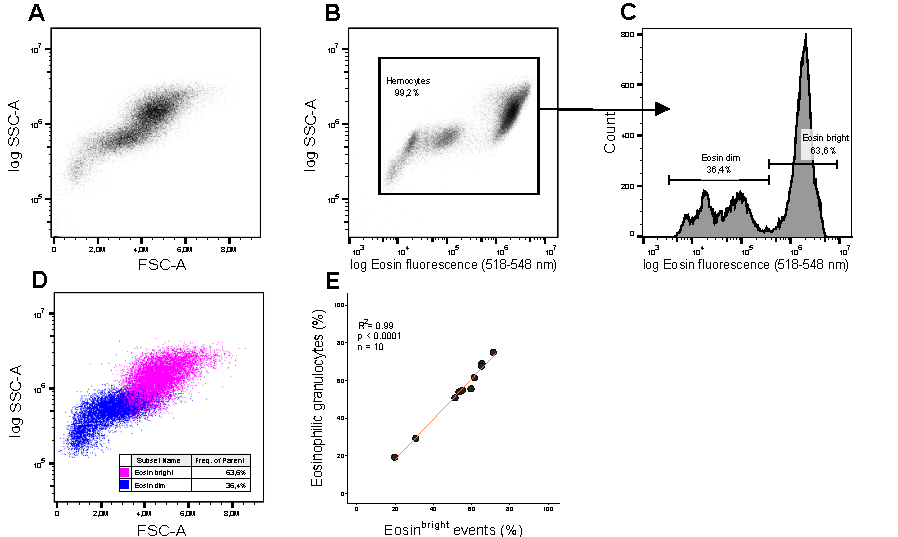
\includegraphics[width=1.0\textwidth]{figures/Gating strategy/Eosin exp big font.pdf}
    \caption{\textbf{Identification eosinophilic granulocytes on FSC vs. SSC dotplots according to log eosin fluorescence (518-548 nm).} Ten formaldehyde-fixed haemolymph samples were stained with 0.5\% eosin and recorded on the flow cytometer right thereafter \textbf{(A)}. Haemocyte events were gated according to log eosin fluorescence vs. SSC-A \textbf{(B)} and the eosin$^{bright}$ events were gated univariately \textbf{(C)}. The eosin$^{bright}$ events were back-gated to show their light scatter profile relative to eosin$^{dim}$ events \textbf{(D)}. The simple regression of eosin$^{bright}$ events (\%) vs. eosinophilic granulocytes (\%) determined from 1000-cell differential counts are shown in \textbf{(E)}, regression line: y$_{i}$ = -3.20042 + 1.06656x$_{i}$.}
    \label{fig:eosin_exp2}
\end{figure}

\subsection{Flow cytometric differential haemocyte count}
\subsubsection{Characterization of haemocytes according calcein efflux and SSC}
\label{subsection:calcein_SSC_char}
After staining with 50 nM \acrshort{calceinam} prior to flow cytometric analyses, suspensions of living haemocytes were separated into three distinct clusters of events according to log calcein fluorescence (518-548 nm) vs. log SSC in 90\% of the untreated adult mussels. As shown in Figure \ref{fig:DHC_gatestrat}C, these clusters corresponded to one subpopulation of calcein dim events with high SSC (calcein$^{-}$/SSC high), one subpopulation of calcein bright events with intermediate SSC (calcein$^{+}$/SSC mid) and one subpopulation of calcein dim events with low SSC-values (calcein$^{-}$/SSC low). The two calcein$^{-}$ clusters were gated according to the regions presented in Figure \ref{fig:DHC_gatestrat}C, and were shown to correspond to cluster 1 and 3 on bivariate plots of FSC vs. log SSC (see Figure \ref{fig:DHC_gatestrat}B and D). Calcein bright events with intermediate SSC-values were gated as events not present in the two aforementioned regions, and were invariably corresponding to cluster 2 when back-gated to bivariate plots of FSC vs. SSC.

The degree of separation between clusters 1-3 were subject to individual variation with regard to log SSC. Since cluster 2 and 3 are distinguished solely on the basis of SSC in light scatter measurements, the events populating these regions could not be completely resolved in mussels where these clusters were partly overlapping with regard to SSC. However, by employing calcein fluorescence as a second discriminator instead of FSC, the haemocytes of cluster 3 could be gated indirectly on the basis of their lower accumulation of hydrolyzed calcein. As the events of cluster 1 also exhibited a lower fluorescent intensity of calcein, the substitution of FSC for calcein fluorescence did not present a compromise for the resolution of cluster 1.

\begin{figure}[H]
    \centering
    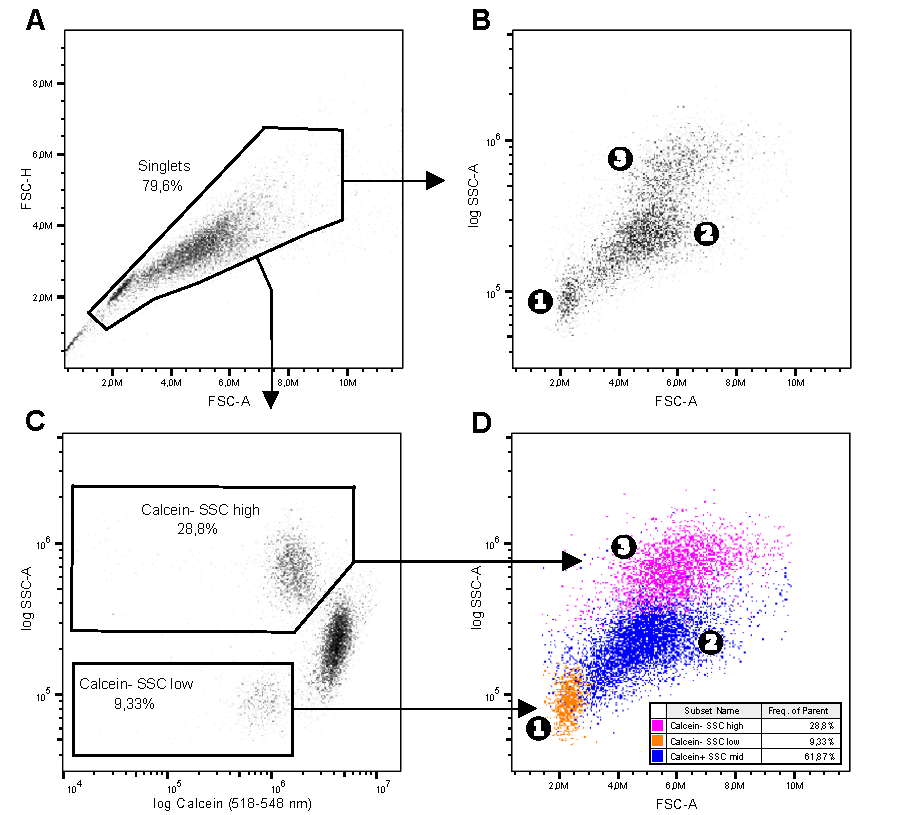
\includegraphics[width=1.0\textwidth]{figures/Gating strategy/SSC Calcein gatestrat full PNG.pdf}
    \caption{ \textbf{Differential haemocyte count gating strategy}. Twenty haemolymph samples withdrawn into ACB (1:1) were stained with 50 nM \acrshort{calceinam} for 15 minutes prior to flow cytometric analysis. \textbf{(A)} Events were gated according to FSC-A vs. FSC-H to eliminate doublet haemocyte events and debris from the analysis. \textbf{(B)} The singlet events populated three distinct clusters according to FSC-A vs. log SSC-A (cluster 1-3). \textbf{(C)} By exchanging FSC-A for log calcein fluorescence on the x-axis, cluster 1 and 3 could be gated without considerable overlap with cluster 2 - due to their lower fluorescent intensity of hydrolyzed \acrshort{calceinam}. \textbf{(D)} The events in the calcein$^{-}$/SSC low and calcein$^{-}$/SSC high gates are shown to correspond to cluster 1 and 3, respectively.}
    \label{fig:DHC_gatestrat}
\end{figure}

\subsubsection{Method validation}
The estimated percentages of small blast-like basophils (events in cluster 1), basophilic granulocytes (events in cluster 2) and eosinophilic granulocytes (events in cluster 3) were highly correlated with the results obtained by traditional microscopic differential counts (Figure \ref{fig:DHC_lin}). The percentage of eosinophilic granulocytes counted in Giemsa-smears were significantly predicted by the percentage of calcein$^{-}$/SSC$^{high}$ events of cluster 3 ($\beta$ = 1.0576, t(18) = 23.8, p<.001), with a mean percent error (MPE) of 6.42$\pm{4}$\% in the flow cytometric estimates. Furthermore, a significant correlation was observed between the results obtained by the two methods (R$^{2}$ = 0.97, F(1, 18) = 566.2, p<.001).

\begin{figure}[H]
    \centering
    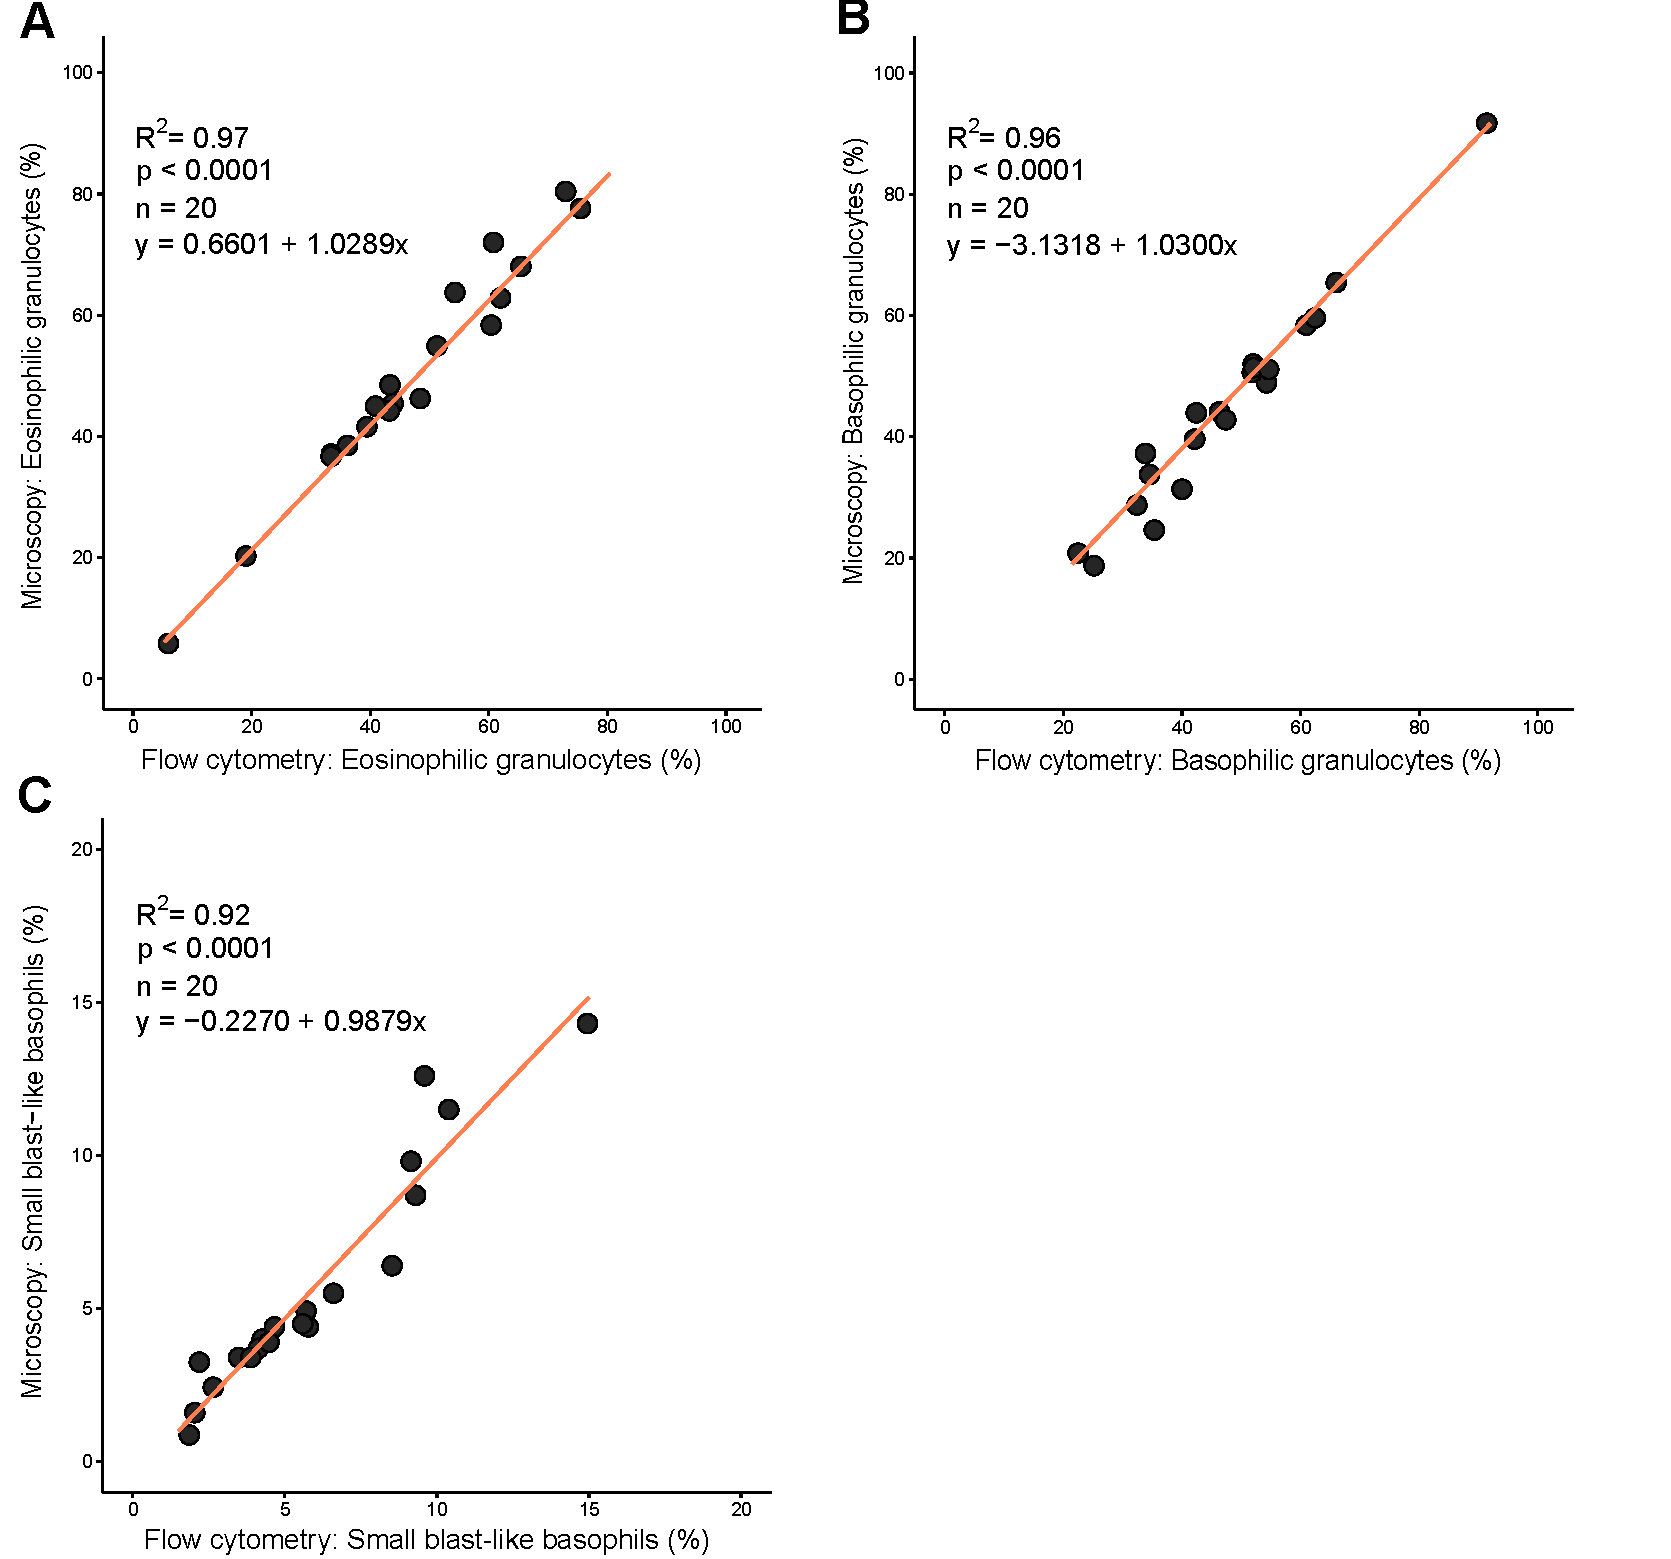
\includegraphics[width=1.0\textwidth]{figures/Gating strategy/SSC Calcein validation.pdf}
    \caption{Correlations between the percentages of eosinophilic granulocytes \textbf{(A)}, basophilic granulocytes \textbf{(B)} and small blast-like basophils \textbf{(C)} from differential haemocyte counts performed by microscopy and flow cytometry (n=20). The three cell types were differentiated as clusters 1-3 (1: small blast-like basophils; 2: basophilic granulocytes; 3: eosinophilic granulocytes), which were gated indirectly according log calcein fluorescence (518-538 nm) vs. log SSC-A as shown in the gating strategy in Figure \ref{fig:DHC_gatestrat}.}
    \label{fig:DHC_lin}
\end{figure}

\noindent The percentages of calcein$^{+}$/SSC$^{mid}$ events of cluster 2 significantly predicted the percentages of basophilic granulocytes from the microscopic counts ($\beta$ = 1.0540, t(18) = 22.0, p<.001). While the correlation between the flow cytometric estimates and the microscopic counts were similar to that of the eosinophilic granulocytes (R$^{2}$ = 0.96, F(1, 18) = 481.9, p<.001); the accuracy were comparatively lower (MPE = 9.80$\pm{12}$\%). As the y-intercept of the best fitted line were marginally lower than zero ($\alpha$ = -5.2120, 95\% CI [-10.2416, -0.1825]), the regression analysis showed that the percentages of basophilic granulocytes were slightly overestimated in the lower end of the observed range. This tendency can be seen from the data depicted in Figure \ref{fig:DHC_lin}B.

The fitted regression model presented in Figure \ref{fig:DHC_lin}C shows that the flow cytometric differential haemocyte count were less accurate in predicting the percentage of small blast-like basophils. This is also evident from the mean percent error of 20.72$\pm{24}$\%. The percentages of calcein$^{-}$/SSC$^{low}$ events in cluster 1 was a significant predictor in most mussels ($\beta$ = 1.0501, t(18) = 14.1, p<.001), but with a few more outliers compared to the other two cell types. Overall, the flow cytometric estimates were significantly correlated with the percentages of blast-like basophils determined my microscopy (R$^{2}$ = 0.92, F(1, 18) = 198.3, p<.001).

\section{Scoring of necrotic haemocytes by flow cytometry}
\subsection{Determination of optimal TO-PRO-3 Iodide staining concentration}
Viable and \ce{MeOH}-killed haemocytes could be separated according to TO-PRO-3 Iodide fluorescence in the whole range of tested concentrations (30 nM - 8 \micro M). As shown in Figure \ref{fig:ToPro3_stain_opt}B, the resolution between ToPro3$^{-}$ and ToPro3$^{+}$ events increased with the TO-PRO$^{TM}$-3 Iodide concentration according to the log-logistic function shown in (\ref{eq:fitted.LL4}), with a marked stagnation > 1.2 \micro M. The model explained almost all the variation in the dataset (Pseudo-R$^{2}$ = 0.99, see table \ref{tb:loglogistic_ToPro3}), and should therefore be a good predictor of the expected resolution between necrotic and viable haemocytes in the tested range of TO-PRO$^{TM}$-3 Iodide.

\begin{equation}
\label{eq:fitted.LL4}
y_{i} = \dfrac{9890700}{1 + (x_i / 0.41655)^{-0.94088}} + \epsilon_i
\end{equation}

\begin{figure}[h]
    \centering
    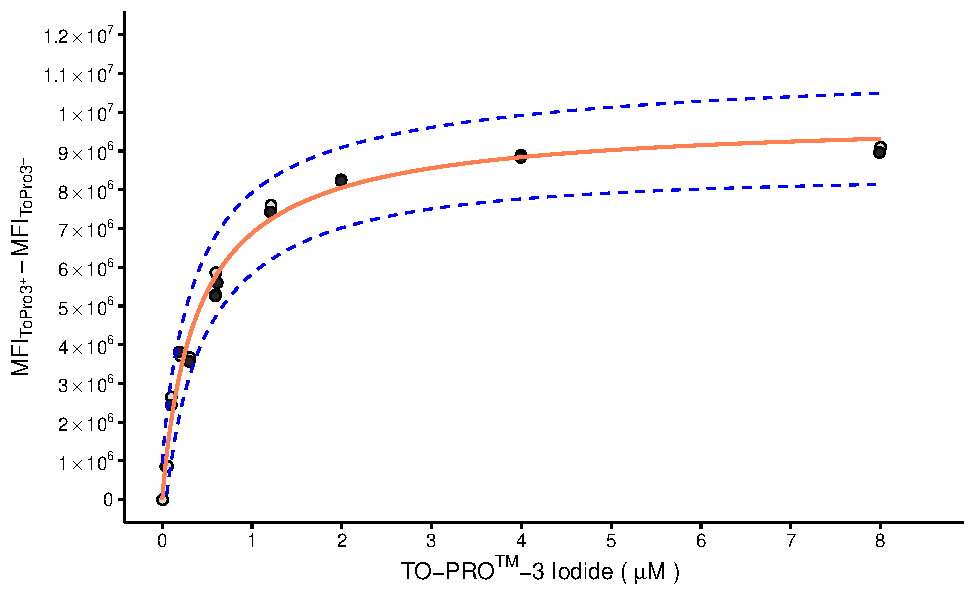
\includegraphics[width=1.0\textwidth]{figures/Method development/ToPro3 LL4.pdf}
    \caption{\textbf{Experimental determination of the optimal TO-PRO$^{TM}$-3 Iodide concentration for a dye exclusion test of membrane integrity}. 10 aliquots of pooled methanol-killed (70\% \ce{MeOH}, 30 min) and viable haemocytes (1:1) were stained with different concentrations of TO-PRO$^{TM}$-3 Iodide (30 nM - 8 \micro M). 640 nm-exited fluorescence from \acrshort{dsdna}-bound TO-PRO$^{TM}$-3 Iodide were collected on the FL4 detector (675/25 nm) of the BD Accuri C6 Plus flow cytometer, recording 10.000 events from each sample after 15 and 30 minute incubation. \textbf{A)} ToPro3$^{-}$ and ToPro3$^{+}$ events were gated on log scale for each sample, \textbf{B)} and their difference in mean fluorescent intensity (MFI) after 15 (\protect\lysegraacircle) and 30 minutes (\protect\darkgraycircle) of incubation were plotted against the concentration of TO-PRO$^{TM}$-3 Iodide. Red line: fitted log-logistic regression model; blue dashed lines: prediction intervals.}
    \label{fig:ToPro3_stain_opt}
\end{figure}

The predicted difference in \acrshort{mfi} at 1.2 \micro M was 7.220.000 (arbitrary units), 95\% PI[6.170.000, 8.260.000]. Since the slope of function \ref{eq:fitted.LL4} decreased rapidly for x > 0.6 \micro M, the predicted difference in MFI at x = 1.2 \micro M was contained within the prediction intervals for the rest of the function's range. Furthermore, the MFI of the ToPro3$^{-}$ populations increased abruptly at concentrations $\geq$ 2 \micro M (see Table \ref{tb:ToPro3_stainopt}, Appendix B), indicating a potential cytotoxic effect of either TO-PRO$^{TM}$-3 Iodide or the \acrshort{dmso} solvent at the three highest concentrations.

Taken together, these results suggested that the potential gain from increasing the staining concentration above 1.2 \micro M was limited, and not completely free of risk. The resolution between viable and necrotic haemocytes was for all practical purposes sufficient in the range of 300 nm - 1.2 \micro M, but the resolution achieved at 1.2 \micro M would simplify gating on a logarithmic scale. 1.2 \micro M TO-PRO$^{TM}$-3 Iodide was therefore preferred for scoring necrotic haemocytes by flow cytometry, together with 50 nM Calcein AM.

The results were also unambiguous regarding the incubation period. According to Figure \ref{fig:ToPro3_stain_opt}B, the resolution between viable and necrotic cells did not increase after the initial 15 minute incubation period. The MFI of necrotic haemocytes did increase somewhat in the extended incubation period, but the resolution remained unchanged due to a concurrent proportional increase among the viable haemocytes (see table \ref{tb:ToPro3_stainopt}, Appendix B). Extending the incubation period beyond 15 minutes would therefore be of little use.

\subsection{Gating strategy}
The finalized quadrant gating strategy for the Calcein AM/TO-PRO$^{TM}$-3 Iodide membrane integrity assay is presented in Figure \ref{fig:TP3_Calcein_gating_strat}. The four plots (A-D) represent samples of viable and methanol-killed haemocytes in equal proportions (A, unstained control; B, Calcein FMO; C, TO-PRO$^{TM}$-3 Iodide FMO; D, Calcein/TO-PRO$^{TM}$-3 Iodide). Unstained controls were used to establish a tentative lower left quadrant gate (Calcein$^{-}$ ToPro3$^{-}$) for non-cellular events. This quadrant was expanded in both directions to include all Calcein$^{-}$ events of the Calcein FMOs and all the ToPro3$^{-}$ events of the TO-PRO$^{TM}$-3 Iodide FMOs (see Figure \ref{fig:TP3_Calcein_gating_strat}B and C). When the double stained samples were run, the viable and methanol-killed haemocytes populated the upper left and lower right quadrants, exclusively (see Figure \ref{fig:TP3_Calcein_gating_strat}D).

\begin{figure}[ht!]
    \centering
    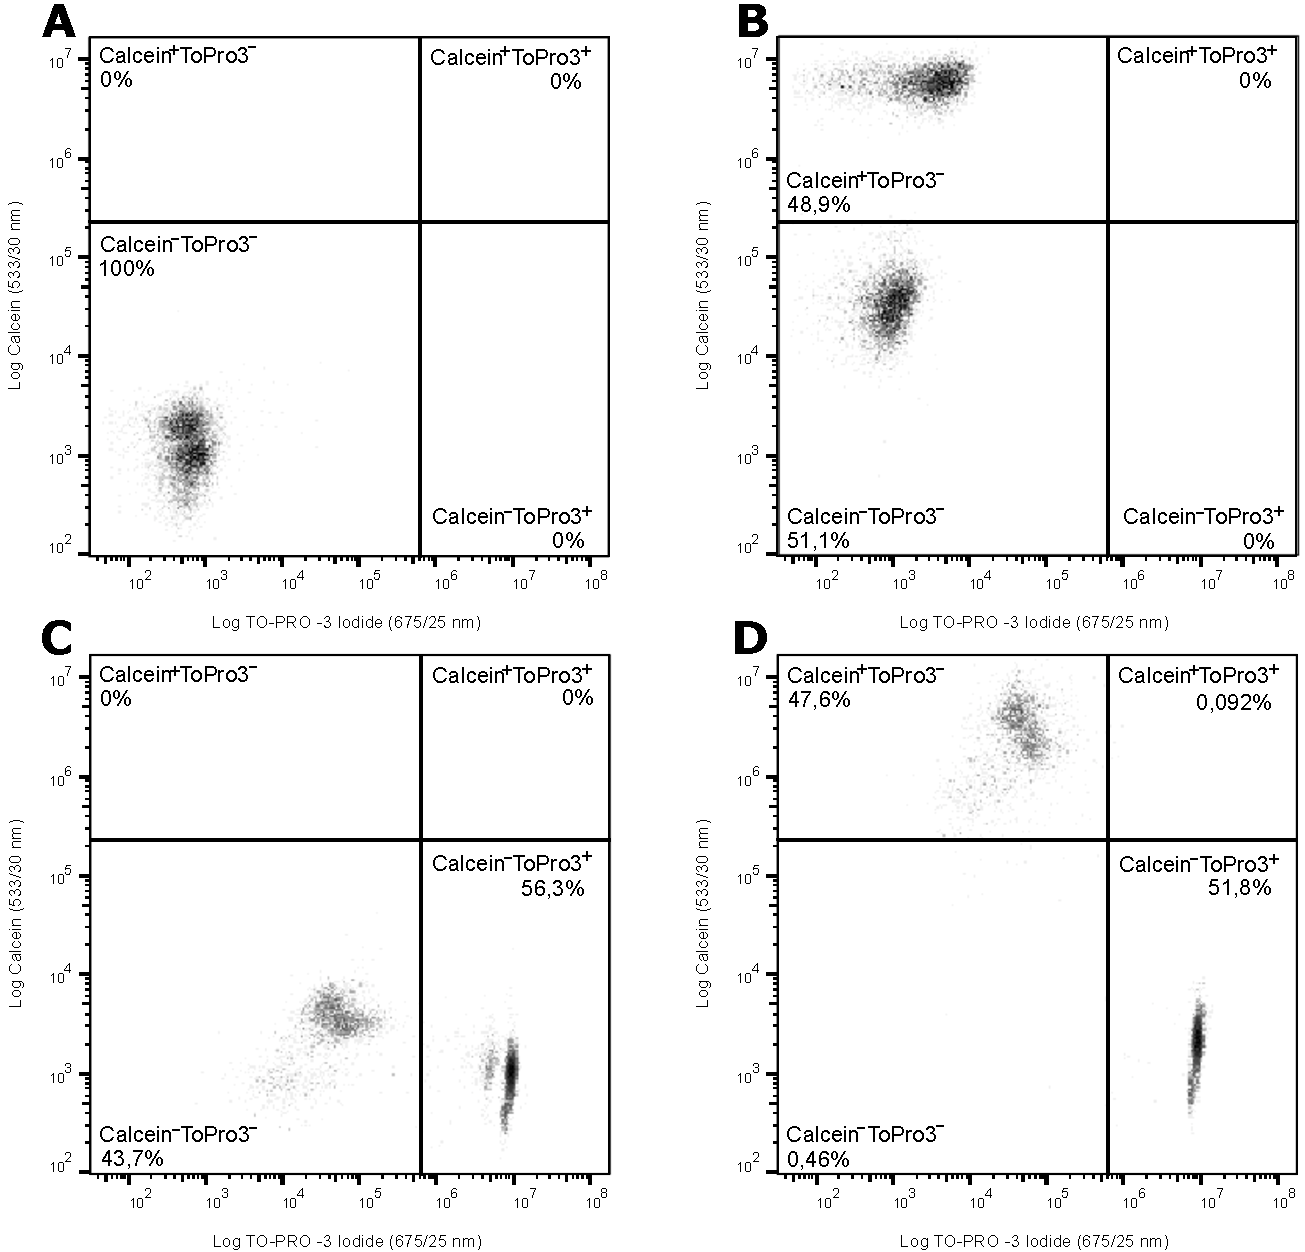
\includegraphics[width=.7\textwidth]{figures/Gating strategy/ToPro3 CAM gating strategy.pdf}
    \caption{\textbf{FL1 (533/30 nm) vs. FL4 (675/25 nm) quadrant gating for flow cytometric scoring of necrotic (Calcein$^{-}$ ToPro3$^{+}$) an viable (Calcein$^{+}$ ToPro3$^{-}$) haemocytes.} By preparing a pool of \ce{MeOH}-killed and newly withdrawn haemocytes in antiaggregative buffer (\acrshort{acb}), gates were drawn according to the florescent profiles of \textbf{A)} Unstained controls, \textbf{B)} Calcein \acrshort{fmo}s, \textbf{C)} TO-PRO$^{TM}$-3 Iodide FMOs and \textbf{D)} aliquotes stained with both probes.}
    \label{fig:TP3_Calcein_gating_strat}
\end{figure}


\subsection{Method validation}
Simple linear regression was used to examine the correlation between results obtained by epifluorescent microscopy and the flow cytometric gating strategy presented in Figure \ref{fig:TP3_Calcein_gating_strat}. It was found that the established quadrant gating strategy significantly predicted the the percentage of ToPro3$^{+}$ haemocytes in samples scored by epifluorescent microscopy ($\beta$ = 0.9882, t(8) = 32.5, p<.001), with a mean absolute error of 2.37$\pm{2}$\% and a mean percent error of 21.8$\pm{35}$\%. The data is presented in Figure \ref{fig:method_val_1}, together with the fitted linear regression model (R$^{2}$ = 0.99, F(1, 8) = 1059, p<.001).

\begin{figure}[ht!]
    \centering
    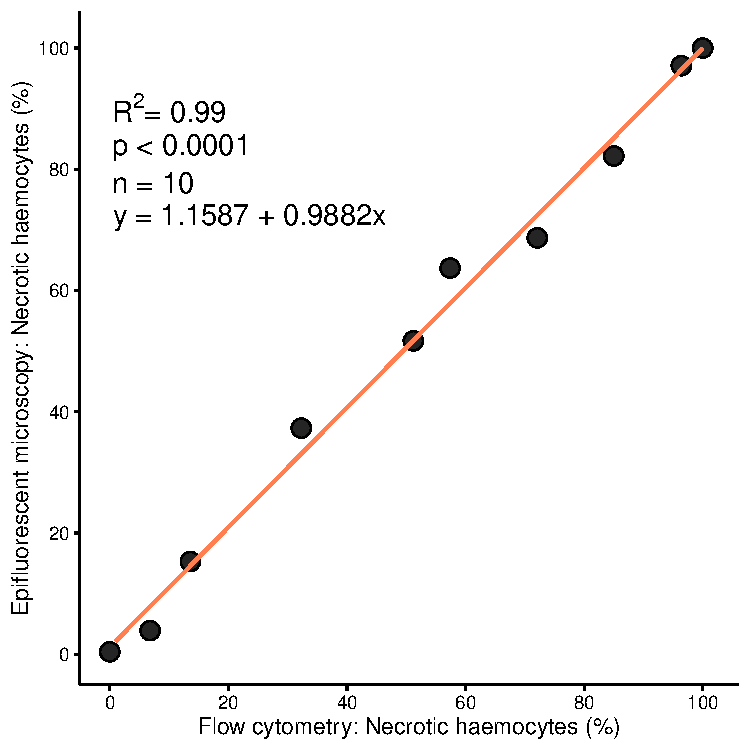
\includegraphics[width=.5\textwidth]{figures/Method development/FCM EM linreg final.pdf}
    \caption{\textbf{Correlation between necrotic haemocyte percentages scored by flow cytometry and epifluorescent microscopy.} 10 samples of freshly withdrawn haemocytes (\acrshort{acb}, 1:1) were mixed with methanol-killed haemocytes in semi-random proportions (0-100\%), stained with Calcein AM (50 nM) and TO-PRO$^{TM}$-3 Iodide (1.2 \micro M) and the percentage of necrotic haemocytes (\%) were scored by both flow cytometry and epifluorescent microscopy. Each datapoint represents one scored sample. Red line: fitted linear regression model.}
    \label{fig:method_val_1}
\end{figure}


\chapter{Discussion}
\label{chap:discuss}

\section{Selection of haemocyte medium for flow cytometric analyses}
Even though the aggregation model was slightly over-dispersed, the estimates provide some insight into the three buffers relative abilities to prevent hemocyte aggregation within the first hour post-withdrawal. The combination of Ca$^{2+}$-free and \acrshort{edta}-containing buffers were effective inhibitors of hemocyte aggregation compared to simply diluting samples on ice. When the latter method was used, visible aggregates were usually formed within the syringes immediately after hemolymph aspiration - even though the \acrshort{mpss} was pre-chilled on ice. This observation shows that a two-fold dilution in MPSS is less than sufficient, such that a further dilution may be required for satisfactory effect. A many-fold dilution would be inconvenient in the preparation of haemolymph smears with a certain desired density, and too time-consuming for the acquisition of 10.000 events on a flow cytometer. This approach was therefore ruled out of question.

By comparing the inhibitory effects of \acrshort{mas} and \acrshort{acb} on haemocyte aggregation, our data suggests the slightly higher concentration of \acrshort{edta} in \acrshort{acb} compensates for the lack of citrate. Since high concentrations of \acrshort{edta} have been reported to impair haemocyte viability (\cite{Grandiosa2018, Burkhard2009}), a direct comparison of \acrshort{mas} and \acrshort{acb} with regards to acute effects on viability was required to identify the most suitable buffer of the two.

Our results suggest that \acrshort{edta} is cytotoxic to haemocytes at the concentrations used in both \acrshort{acb} (13.4 mM) and \acrshort{mas} (11.5 mM), since these buffers caused a significant dose-dependent increase in the percentage of necrotic haemocytes across the three timepoints (Table \ref{tb:Paired_ttests}). However, since there was no significant differences between the \acrshort{edta}-containing buffers and the negative control group after 15 minutes of incubation, this cytotoxic effect had no detectable manifestation within the time-frame of the planned flow cytometric assay. As long as haemolymph samples are stained and processed within 30 minutes of sampling, a flow cytometric dye exclusion/inclusion assay with TO-PRO$^{TM}$-3 Iodide and \acrshort{calceinam} will not have time to detect \emph{in vitro} necrosis caused by the buffers themselves.

The apoptosis assay with non-adjusted MAS (pH = 6.1) showed that 15 minutes was more than enough for haemocytes to enter programmed cell death. The percentage of cells already in late apoptosis suggests that an abrupt decrease in pH is an efficacious inducer of apoptosis, and that the haemocytes of \emph{M. edulis} are very sensitive to the environmental pH. This has been demonstrated by several recent studies investigating the effects of ocean acidification on the immune system of bivalves (see e.g., \cite{Wang2016, Dang2023}). Maintaining the pH of MAS at 6.1 is therefore not an option for flow cytometric analyses of apotosis or necrosis.

Our analyses did not detect any differences between ACB and MAS (pH = 7.0) with regard to their anticoagulant effects or cytotoxicity within the time-frame of the planned assays. The data does however demonstrate the importance of a carefully regulated haemocyte medium pH. As the buffer capacity of pH-adjusted MAS is negligible, ACB appears as the most suitable haemocyte medium of the two. The Anticoagulant Buffer (ACB) of Pipe et al. (1997) was therefore used for flow cytometric analyses in the Hybrid MN Cytome Assay.

\section{Development of a flow cytometric differential count}
The haemolymph of \emph{M. edulis} were found to contain three morphologically distinct cell types according to traditional cytological criteria. These comprised (1) small agranular basophilic cells (blast-like basophils), (2) larger basophilic cells with small inconspicuous granules (basophilic granulocytes) and (3) large eosinophilic cells with cytoplasm densely populated by larger eosinophilic granules (eosinophilic granulocytes). There has been scientific dispute regarding the classification of basophilic and eosinophilic granulocytes as two distinct cell-types (\cite{Cheng1980}), however; this distinction is made for purely descriptive purposes herein.

Similar to the cytological characterization, a maximum of three distinct subpopulations could be separated according to relative size (FSC) and internal complexity (SSC) in suspensions of living haemocytes. These comprised one subpopulation of small cells with low internal complexity (cluster 1), one subpopulation of larger cells with intermediate internal complexity (cluster 2) and one subpopulation of large cells with high internal complexity (cluster 3). The apparent correlation between these subpopulations and the three cell types were striking with regard to their relative sizes and granularity.

The small blast-like basophils (5.63 $\pm{0.72}$ \micro m) were considerably smaller than the basophilic and eosinophilic granulocytes, and exhibited no apparent granulation. One would therefore expect them to be unambiguously separated from the larger granulocytes according to both \acrshort{fsc} and \acrshort{ssc}. The size distributions in Figure \ref{fig:Diameters} does however indicate an overlap in size between the largest blast-like basophils and the smallest basophillic granulocytes in some mussels. But, since they are uncomplex cells, they should be separated according to \acrshort{ssc} regardless. The events populating cluster 1 in Figure \ref{fig:fsc_vs_ssc} were therefore expected to represent small blast-like basophilic haemocytes. 

Both eosinophilic and basophilic granulocytes were granulated in the formal definition of the word. But this discussion requires a more nuanced interpretation of what is meant by granulocyte herein. The cytoplasm of eosinophilic granulocytes were packed with pink to dark purple granules to the extent that their cytoplasm appeared pink in a non-spread state (see Figure \ref{fig:celltypes}, K-O). This stands in sharp contrast to the granulation of basophilic granulocytes, which were more sparse, variable and much less conspicuous. Consequently, there is little doubt that cluster 3 is expected to correspond to eosinophilic granulocytes, while the semi-granular events of \emph{\emph{cluster 2}} aligns with the size and complexity of basophilic granulocytes.

As seen from the size distributions in Figure \ref{fig:Diameters}, the basophilic and eosinophilic granulocytes were not readily distinguishable according to cell size. That result was further substantiated by the fact that cluster 2 and 3 had substantially overlapping \acrshort{fsc}-values. The haemolymph samples depicted in Figure \ref{fig:fsc_vs_ssc} does however show that the \acrshort{fsc} of cluster 3 is slightly right-shifted relative to cluster 2, which is expected since the eosinophilic granulocytes were found to be 0.92 \micro M larger than basophilic granulocytes on average.

Even thought there was an apparent correlation between cluster 1-3 and the size and internal complexity of the cytologically defined cell types; these interpretations required visual verification before a potential gating strategy could be implemented from these results. The ispycnic separation of eosinophilic granulocytes from the two basophilic cell types allowed for these cell types to be characterized by FSC vs. SSC separately.

The eosinophilic granulocytes (> 96\%) formed a dense cluster of events with high SSC relative to the two basophilic cell types, and were thus positively identified as the cells populating cluster 3 in figure \ref{fig:fsc_vs_ssc}. This observation was further supported by the fact that eosin$^{bright}$ events populated the same cluster when samples of formaldehyde-fixed cells stained with 0.5\% eosin were back-gated to bivariate plots of FSC vs. SSC. Since there was a strong correlation between eosin$^{bright}$ events (\%) and the percentage of eosinophilic granulocytes (R$^{2}$=0.99), this finding also provides solid evidence for this hypothesis. The same conclusion was reached by LeFoll et al., (2010), from which the latter experiment originated.

Similar to the findings of previous investigators (\cite{Friebel1995, Pipe1997, Carballal1997}), the basophilic granulocytes and small blast-like basophils of \emph{M. edulis} were not separated according to density by the discontinuous Percoll gradient. This finding demonstrates that the granule density of basophilic granulocytes is insufficient to produce measurable difference in the overall density of the two basophilic cell types. However, the basophilic cells that populated the middle fraction of the gradient were separated into two subpopulations according to FSC vs. SSC in the subsequent flow cytometric analyses (Figure \ref{fig:Percoll-dotplots}C). These subpopulations occupied the regions corresponding to cluster 1 and cluster 2 in suspensions of living haemocytes, and eosin$^{dim}$ events in the measurements of eosin fluorescence. Based on the relative size and granularity of these cell types, cluster 2 should intuitively correspond to larger basophilic granulocytes, while cluster 1 to that of small blast-like basophils.

Since the two basophilic cell types were not separable according to density, this theory could not be tested directly without access to a flow cytometer with cell-sorting capabilities. Instead, the theory was provided with support from simple linear regression analyses of the flow cytometric differential haemocyte count estimates, where the percentages of events populating cluster 1 and 2 were regressed on the percentages of small blast-like basophils and basophilic granulocytes determined by microscopic counts from the same mussels, respectively. The results demonstrated that there is a direct linear relationship between the percentage of events in cluster 1 and small blast-like basophils in a mussel (R$^{2}$ = 0.92), with the same being true for the percentage of events in cluster 2 and basophilic granulocytes (R$^{2}$ = 0.96).

As pointed out in section \ref{subsection:Results_FlowChar} and \ref{subsection:calcein_SSC_char}, light-scatter analyses of haemolymph from \emph{M. edulis} did not always result in three well defined subpopulations, i.e., cluster 1-3. This was largely brought about by the substantial overlap between the two granular cell types (cluster 2 and 3) according to FSC, which made it hard to gate these cell types accurately when they were not completely separated according to SSC. In context of developing a flow cytometric differential haemocyte count for \emph{M. edulis}, this fact presented a challenge for the application of FSC vs. log SSC as the only discriminators. Careful staining with eosin represented a potential candidate, as the percentage of eosin$^{bright}$ events had proven to be a good predictor for the percentage eosinophilic granulocytes in formaldehyde-fixed samples. The two centrifugation steps and fixation (1 hour) did however render this methodology rather time-consuming, such that a cell-permeable fluorescent probe would be more preferable.

The cell-permeable fluorescent probe \acrshort{calceinam} were shown to produce dimmer signals in eosinophilic granulocytes and small blast-like basophils compared to the basophilic granulocytes. This phenomenon was explained by the work of Rioult et al., (2014), who demonstrated that \acrshort{calceinam} is a substrate of the Multidrug Resistance-related Protein (MRP) efflux pump in \emph{M. edulis}, which has higher expression and inducibility in eosinophilic granulocytes. The lower fluorescent intensity of hydrolyzed calcein observed in small blast-like basophils can possibly be explained by their smaller size (cell volume), as the fluorescent signals were not normalized to FSC, and Rioult et al., (2014) showed that the \acrshort{calceinam} efflux activity were similar in the two basophilic cell types.

By gating the small blast-like basophils (calcein$^{-}$/SSC$^{low}$), basophilic granulocytes (calcein$^{+}$/SSC$^{mid}$) and eosinophilic granulocytes (calcein$^{-}$/SSC$^{high}$) of cluster 1-3 according to log SSC and their differential accumulation of hydrolyzed calcein, the three cell types could be distinguished by flow cytometry in 90\% of the mussels tested (n=22). Even though SSC constituted the primary discriminator between the three cell types, their differential abilities to efflux \acrshort{calceinam} resulted in a practically applicable resolution, which allowed the events of cluster 1-3 to be gated in spite of partial or substantial overlaps according to SSC. The flow cytometric differential haemocyte count

\section{Scoring of necrotic haemocytes by flow cytometry}

Early early apoptotic cells take up ToPro3 through PANX1 channels before PS externalization (\cite{Poon2014}). ToPro3+/Apo15- haemocytes are thus also early apoptotic cells, and not necrotic - as necrotic cells are double positive (\cite{Jiang2016, Feng2021}).




\section{Scoring of apoptotic haemocytes by flow cytometry}

\chapter{Conclusion}




%\newpage
%\chapter{Bibliography}
%\bibliographystyle{unsrtnat}  %Definerer bibliografistil
%{\footnotesize\bibliography{mendeley-entrans.bib, manual-bibtex.bib}}

\chapter*{\bibname}
\printbibliography[heading=none]


\appendix
\chapter{Additional Material}
\label{app:additional}



Additional material that does not fit in the main thesis but may still be relevant to share, e.g., raw data from experiments and surveys, code listings, additional plots, pre-project reports, project agreements, contracts, logs etc., can be put in appendices. Simply issue the command \texttt{\textbackslash appendix} in the main \texttt{.tex} file, and make one chapter per appendix.

If the appendix is in the form of a ready-made PDF file, it should be supported by a small descriptive text, and included using the \texttt{pdfpages} package. To illustrate how it works, a standard project agreement (for the IE faculty at NTNU in Gjøvik) is attached here. You would probably want the included PDF file to begin on an odd (right hand) page, which is achieved by using the \texttt{\textbackslash cleardoublepage} command immediately before the \texttt{\textbackslash includepdf[]\{\}} command. Use the option \texttt{[pages=-]} to include all pages of the PDF document, or, e.g., \texttt{[pages=2-4]} to include only the given page range.
\chapter{Raw data}
\label{app:rawdata}


\section{Method development: raw data}
\subsection{Hemocyte medium proportion aggregation data}

\begin{center}
\begin{longtable}{ccccc}
\caption{The buffer aggregation proportion raw data longtable.}\label{tab:long_table1} \\
\hline
Mussel ID & Buffer & t (min) & $N_{tx}$ & $N_{t0}$ \\
\hline 
\endfirsthead

\multicolumn{5}{c}%
{{\bfseries \tablename\ \thetable{} -- continued from previous page}} \\

\hline
Mussel ID & Buffer & t (min) & $N_{tx}$ & $N_{t0}$ \\ 
\hline 
\endhead

\hline \multicolumn{5}{|r|}{{Continued on next page}} \\ \hline
\endfoot

\hline \hline
\endlastfoot	
M1	&	MAS	&	0.000001	&	36877	&	36877	\\
M1	&	MAS	&	19	&	23728	&	36877	\\
M1	&	MAS	&	49	&	13479	&	36877	\\
M1	&	MAS	&	78	&	5209	&	36877	\\
M2	&	MAS	&	0.000001	&	25544	&	25544	\\
M2	&	MAS	&	15	&	17570	&	25544	\\
M2	&	MAS	&	45	&	8195	&	25544	\\
M2	&	MAS	&	69	&	5060	&	25544	\\
M3	&	MAS	&	0.000001	&	24381	&	24381	\\
M3	&	MAS	&	16	&	21462	&	24381	\\
M3	&	MAS	&	47	&	9347	&	24381	\\
M3	&	MAS	&	67	&	8525	&	24381	\\
M4	&	MAS	&	0.000001	&	27327	&	27327	\\
M4	&	MAS	&	15	&	26100	&	27327	\\
M4	&	MAS	&	30	&	22529	&	27327	\\
M4	&	MAS	&	59	&	8333	&	27327	\\
M5	&	MAS	&	0.000001	&	12889	&	12889	\\
M5	&	MAS	&	15	&	10605	&	12889	\\
M5	&	MAS	&	30	&	8146	&	12889	\\
M5	&	MAS	&	60	&	3450	&	12889	\\
M6	&	MAS	&	0.000001	&	2519	&	2519	\\
M6	&	MAS	&	45	&	2107	&	2519	\\
M6	&	MAS	&	70	&	1627	&	2519	\\
M7	&	MAS	&	0.000001	&	4131	&	4131	\\
M7	&	MAS	&	45	&	2622	&	4131	\\
M7	&	MAS	&	69	&	2149	&	4131	\\
A1	&	ACB	&	0.000001	&	876	&	876	\\
A1	&	ACB	&	19	&	504	&	876	\\
A1	&	ACB	&	37	&	477	&	876	\\
A1	&	ACB	&	67	&	344	&	876	\\
A2	&	ACB	&	0.000001	&	6835	&	6835	\\
A2	&	ACB	&	17	&	5430	&	6835	\\
A2	&	ACB	&	34	&	3411	&	6835	\\
A2	&	ACB	&	64	&	3942	&	6835	\\
A3	&	ACB	&	0.000001	&	14829	&	14829	\\
A3	&	ACB	&	17	&	13764	&	14829	\\
A3	&	ACB	&	32	&	8520	&	14829	\\
A3	&	ACB	&	63	&	4579	&	14829	\\
A4	&	ACB	&	0.000001	&	48859	&	48859	\\
A4	&	ACB	&	15	&	44741	&	48859	\\
A4	&	ACB	&	30	&	31079	&	48859	\\
A4	&	ACB	&	60	&	11281	&	48859	\\
A5	&	ACB	&	0.000001	&	5641	&	5641	\\
A5	&	ACB	&	15	&	3079	&	5641	\\
A5	&	ACB	&	30	&	2466	&	5641	\\
A5	&	ACB	&	45	&	2413	&	5641	\\
A6	&	ACB	&	0.000001	&	10140	&	10140	\\
A6	&	ACB	&	15	&	8912	&	10140	\\
A6	&	ACB	&	30	&	5353	&	10140	\\
A6	&	ACB	&	45	&	3681	&	10140	\\
A7	&	ACB	&	0.000001	&	39534	&	39534	\\
A7	&	ACB	&	17	&	20087	&	39534	\\
A7	&	ACB	&	32	&	14581	&	39534	\\
A7	&	ACB	&	47	&	10109	&	39534	\\
A8	&	ACB	&	0.000001	&	16736	&	16736	\\
A8	&	ACB	&	15	&	11449	&	16736	\\
A8	&	ACB	&	30	&	8935	&	16736	\\
A8	&	ACB	&	45	&	5145	&	16736	\\
H1	&	MPSS	&	0.000001	&	2447	&	2447	\\
H1	&	MPSS	&	15	&	823	&	2447	\\
H1	&	MPSS	&	30	&	887	&	2447	\\
H1	&	MPSS	&	45	&	972	&	2447	\\
H1	&	MPSS	&	60	&	798	&	2447	\\
H2	&	MPSS	&	0.000001	&	2645	&	2645	\\
H2	&	MPSS	&	15	&	1693	&	2645	\\
H2	&	MPSS	&	30	&	1779	&	2645	\\
H2	&	MPSS	&	45	&	1438	&	2645	\\
H2	&	MPSS	&	60	&	1419	&	2645	\\
H3	&	MPSS	&	0.000001	&	2377	&	2377	\\
H3	&	MPSS	&	15	&	1318	&	2377	\\
H3	&	MPSS	&	30	&	1064	&	2377	\\
H3	&	MPSS	&	45	&	862	&	2377	\\
H3	&	MPSS	&	60	&	659	&	2377	\\
H4	&	MPSS	&	0.000001	&	2879	&	2879	\\
H4	&	MPSS	&	15	&	1624	&	2879	\\
H4	&	MPSS	&	30	&	1617	&	2879	\\
H4	&	MPSS	&	45	&	1049	&	2879	\\
H4	&	MPSS	&	60	&	1120	&	2879	\\
H5	&	MPSS	&	0.000001	&	3151	&	3151	\\
H5	&	MPSS	&	15	&	1445	&	3151	\\
H5	&	MPSS	&	30	&	1125	&	3151	\\
H5	&	MPSS	&	45	&	984	&	3151	\\
H5	&	MPSS	&	60	&	414	&	3151	\\
H6	&	MPSS	&	0.000001	&	1699	&	1699	\\
H6	&	MPSS	&	15	&	1080	&	1699	\\
H6	&	MPSS	&	31	&	733	&	1699	\\
H6	&	MPSS	&	45	&	811	&	1699	\\
H6	&	MPSS	&	60	&	715	&	1699	\\
H7	&	MPSS	&	0.000001	&	3309	&	3309	\\
H7	&	MPSS	&	15	&	1634	&	3309	\\
H7	&	MPSS	&	31	&	1453	&	3309	\\
H7	&	MPSS	&	46	&	1415	&	3309	\\
H7	&	MPSS	&	60	&	1393	&	3309	\\
H8	&	MPSS	&	0.000001	&	2822	&	2822	\\
H8	&	MPSS	&	15	&	1460	&	2822	\\
H8	&	MPSS	&	30	&	1518	&	2822	\\
H8	&	MPSS	&	45	&	1475	&	2822	\\
H8	&	MPSS	&	60	&	1346	&	2822	\\
\end{longtable}    
\end{center}

\pagebreak


\subsection{Hemocyte medium viability raw data}

\begin{center}
\begin{longtable}{cccccc}
\caption{The buffer viability raw data longtable.} \label{tab:long_table2} \\
\hline
\multirow{2}{*}{Buffer} & \multirow{2}{*}{Incubation} & \multicolumn{4}{c}{Count} \\
  && CAM$^{+}$ TP3$^{-}$ & CAM$^{+}$ TP3$^{+}$ & CAM$^{-}$TP3$^{+}$ & CAM$^{-}$ TP3$^{-}$ \\ 
\hline 
\endfirsthead

\multicolumn{6}{c}%
{{\bfseries \tablename\ \thetable{} -- continued from previous page}} \\

\hline
\multirow{2}{*}{Buffer} & \multirow{2}{*}{Incubation} & \multicolumn{4}{c}{Count} \\
 && CAM$^{+}$ TP3$^{-}$ & CAM$^{+}$ TP3$^{+}$ & CAM$^{-}$TP3$^{+}$ & CAM$^{-}$ TP3$^{-}$ \\ 
\hline 
\endhead

\hline \multicolumn{6}{|r|}{{Continued on next page}} \\ \hline
\endfoot

\hline \hline
\endlastfoot
ACB	&	15 min	&	9957	&	1	&	28	&	12	\\
ACB	&	15 min	&	9907	&	12	&	44	&	1	\\
ACB	&	15 min	&	9970	&	1	&	27	&	8	\\
ACB	&	15 min	&	9942	&	8	&	34	&	32	\\
ACB	&	15 min	&	9925	&	7	&	45	&	10	\\
ACB	&	15 min	&	9946	&	5	&	17	&	3	\\
ACB	&	15 min	&	9989	&	1	&	16	&	3	\\
ACB	&	15 min	&	9970	&	9	&	23	&	6	\\
MPSS	&	15 min	&	7707	&	3	&	5	&	4	\\
MPSS	&	15 min	&	6622	&	3	&	8	&	5	\\
MPSS	&	15 min	&	5748	&	8	&	20	&	3	\\
MPSS	&	15 min	&	10040	&	0	&	30	&	57	\\
MPSS	&	15 min	&	9937	&	1	&	13	&	49	\\
MPSS	&	15 min	&	9929	&	2	&	24	&	45	\\
MPSS	&	15 min	&	9950	&	0	&	32	&	18	\\
MPSS	&	15 min	&	9970	&	2	&	15	&	13	\\
MAS	&	15 min	&	8600	&	1	&	15	&	8	\\
MAS	&	15 min	&	9033	&	0	&	30	&	5	\\
MAS	&	15 min	&	8340	&	1	&	9	&	7	\\
MAS	&	15 min	&	8633	&	0	&	7	&	12	\\
MAS	&	15 min	&	7901	&	2	&	17	&	3	\\
MAS	&	15 min	&	8863	&	0	&	10	&	1	\\
MAS	&	15 min	&	9133	&	3	&	17	&	2	\\
MAS	&	15 min	&	8929	&	0	&	12	&	12	\\
ACB	&	2 hours	&	9457	&	4	&	62	&	252	\\
ACB	&	2 hours	&	9792	&	12	&	67	&	70	\\
ACB	&	2 hours	&	9984	&	4	&	58	&	109	\\
ACB	&	2 hours	&	1829	&	0	&	16	&	11	\\
ACB	&	2 hours	&	6801	&	2	&	21	&	237	\\
ACB	&	2 hours	&	4403	&	0	&	17	&	307	\\
ACB	&	2 hours	&	9752	&	5	&	86	&	241	\\
ACB	&	2 hours	&	9875	&	5	&	34	&	123	\\
MPSS	&	2 hours	&	9276	&	21	&	12	&	56	\\
MPSS	&	2 hours	&	6279	&	14	&	2	&	39	\\
MPSS	&	2 hours	&	4869	&	3	&	3	&	43	\\
MPSS	&	2 hours	&	4680	&	13	&	4	&	414	\\
MPSS	&	2 hours	&	6174	&	4	&	0	&	60	\\
MPSS	&	2 hours	&	7573	&	6	&	5	&	37	\\
MPSS	&	2 hours	&	8131	&	25	&	6	&	103	\\
MPSS	&	2 hours	&	8930	&	10	&	0	&	93	\\
MAS	&	2 hours	&	5061	&	0	&	28	&	64	\\
MAS	&	2 hours	&	4947	&	2	&	39	&	103	\\
MAS	&	2 hours	&	9973	&	11	&	62	&	58	\\
MAS	&	2 hours	&	6190	&	8	&	14	&	74	\\
MAS	&	2 hours	&	8473	&	0	&	21	&	104	\\
MAS	&	2 hours	&	9884	&	8	&	64	&	118	\\
MAS	&	2 hours	&	9930	&	5	&	22	&	124	\\
MAS	&	2 hours	&	9953	&	0	&	28	&	19	\\
ACB	&	20 hours	&	9135	&	8	&	541	&	206	\\
ACB	&	20 hours	&	7519	&	1	&	1559	&	341	\\
ACB	&	20 hours	&	7383	&	4	&	994	&	594	\\
ACB	&	20 hours	&	9668	&	7	&	340	&	285	\\
ACB	&	20 hours	&	10054	&	2	&	143	&	134	\\
ACB	&	20 hours	&	9103	&	27	&	637	&	118	\\
ACB	&	20 hours	&	8198	&	4	&	896	&	234	\\
ACB	&	20 hours	&	8174	&	2	&	969	&	328	\\
MPSS	&	20 hours	&	9577	&	29	&	51	&	7	\\
MPSS	&	20 hours	&	9277	&	11	&	371	&	33	\\
MPSS	&	20 hours	&	9651	&	12	&	41	&	11	\\
MPSS	&	20 hours	&	9355	&	22	&	149	&	12	\\
MPSS	&	20 hours	&	9879	&	9	&	59	&	23	\\
MPSS	&	20 hours	&	9736	&	89	&	69	&	56	\\
MPSS	&	20 hours	&	9933	&	2	&	18	&	8	\\
MPSS	&	20 hours	&	9693	&	6	&	158	&	32	\\
MAS	&	20 hours	&	8025	&	24	&	523	&	578	\\
MAS	&	20 hours	&	8910	&	3	&	382	&	210	\\
MAS	&	20 hours	&	8502	&	1	&	453	&	523	\\
MAS	&	20 hours	&	9663	&	4	&	370	&	417	\\
MAS	&	20 hours	&	8959	&	16	&	1088	&	607	\\
MAS	&	20 hours	&	9640	&	3	&	446	&	467	\\
MAS	&	20 hours	&	8537	&	6	&	675	&	309	\\
MAS	&	20 hours	&	9237	&	10	&	1033	&	685	\\

\end{longtable}    
\end{center}

\subsection{Experimental determination of optimal TO-PRO-3 Iodide concentration}

The raw data from the experimental determination of an optimal TO-PRO$^{TM}$-3 Iodide concentration for a flow cytometric dye exclusion test is shown in table \ref{tb:ToPro3_stainopt}. The estimated parameters of the fitted log-logistic model are presented in \ref{tb:loglogistic_ToPro3}.


\begin{table}[H]
	\centering
	\caption{Raw data from the experimental determination of the optimal range of TO-PRO$^{TM}$-3 Iodide concentrations for a flow cytometric dye exclusion test of membrane integrity. The table lists the TO-PRO$^{TM}$-3 concentrations tested (\micro M),  incubation durations (min), the mean fluorescent intensity (MFI) of viable (ToPro$^{-}$) and \ce{MeOH}-killed haemocytes (ToPro$^{+}$) and the difference between the two (MFI$_{ToPro3^{+}}$ - MFI$_{ToPro3^{-}}$). Samples were analyzed on a BD Accuri C6 Plus flow cytometer (BD Biosciences, California, US) and MFI's were calculated using FlowJo$^{TM}$ v10.8 Software (BD Life Sciences).}
	\label{tb:ToPro3_stainopt}
	\resizebox{\linewidth}{!}{
	\begin{tabular}{ccccc}
        \toprule
	    \multirow{2}[-5]{*}{TO-PRO$^{TM}$-3 Iodide} & \multirow{2}[-5]{*}{Incubation} & \multicolumn{2}{c}{Mean Fluorescent Intensity} & \multirow{2}{*}{MFI$_{ToPro3^{+}}$ - MFI$_{ToPro3^{-}}$} \\
        (\micro M) & (min) & ToPro3$^{+}$ & ToPro3$^{-}$ & \\
		\midrule
  0     &   15  &    764    &   554     &   210 \\
0.03	&	15	&	867000	&	6750	&	860250	\\
0.06	&	15	&	865000	&	6488	&	858512	\\
0.1	&	15	&	2670000	&	19378	&	2650622	\\
0.3	&	15	&	3710000	&	43720	&	3666280	\\
0.2	&	15	&	3750000	&	41441	&	3708559	\\
0.6	&	15	&	5920000	&	62519	&	5857481	\\
0.6	&	15	&	5330000	&	40903	&	5289097	\\
1.2	&	15	&	7700000	&	103179	&	7596821	\\
2	&	15	&	8550000	&	298543	&	8251457	\\
4	&	15	&	9240000	&	352373	&	8887627	\\
8	&	15	&	9550000	&	456001	&	9093999	\\
0.1	&	30	&	2470000	&	28374	&	2441626	\\
0.2	&	30	&	3860000	&	48720	&	3811280	\\
0.3	&	30	&	3640000	&	68309	&	3571691	\\
0.6	&	30	&	5690000	&	94568	&	5595432	\\
0.6	&	30	&	5320000	&	60620	&	5259380	\\
1.2	&	30	&	7580000	&	155710	&	7424290	\\
2	&	30	&	8710000	&	486028	&	8223972	\\
4	&	30	&	9410000	&	577181	&	8832819	\\
8	&	30	&	9670000	&	713160	&	8956840	\\
   		\bottomrule
	\end{tabular}
}
\end{table}


\begin{table}[H]
	\centering
	\caption{Log-logistic regression analysis of the relationship between TO-PRO$^{TM}$-3 Iodide concentration and the difference in median fluorescent intensity (MFI) between ToPro3$^{-}$ and ToPro3$^{-}$ populations. Parameter estimates with 95\% CI, standard errors, t-value and the belonging p-value.}
	\label{tb:loglogistic_ToPro3}
	\resizebox{\linewidth}{!}{
	\begin{tabular}{cccccc}
        \toprule
	\textbf{Parameter} & \textbf{Estimate} & \textbf{95\% CI} & \textbf{Std. Error} & \textbf{t-value} & \textbf{Pr(T > $\mid$ t $\mid)$} \\
		\midrule
  \emph{b} & -0.94088 & [-1.182762, -0.6989903] & 0.11 & -8.7992 & < 0.001 \\
  \emph{d} & 9890700  & [8701569, 11079860]     & 530000 & 18.8155 & < 0.001 \\
  \emph{e} & 0.41655  & [0.2622887, 0.5708113]  & 0.068 & 6.10085 & < 0.001 \\
  &&&&& \\
  \multicolumn{6}{l}{Pseudo R$^{2}$ = 0.99} \\
  \multicolumn{6}{l}{Residual standard error: 416074.3 on 9 degrees of freedom} \\
		\bottomrule
	\end{tabular}
	}
\end{table}



Pseudo-R$^{2}$ by (\cite{Shabenberger2002}), which the statistic used by the \emph{R2nls} function for .nls and .drm type objects in the \emph{aomisc} package in R.

\begin{equation}
\label{eq:PseudoR2}
Pseudo ~ R^2 = 1 - \dfrac{SS_{res}}{SS_{tot}}
\end{equation}



\end{document}
